% Options for packages loaded elsewhere
% Options for packages loaded elsewhere
\PassOptionsToPackage{unicode}{hyperref}
\PassOptionsToPackage{hyphens}{url}
\PassOptionsToPackage{dvipsnames,svgnames,x11names}{xcolor}
%
\documentclass[
  letterpaper,
  DIV=11,
  numbers=noendperiod]{scrreprt}
\usepackage{xcolor}
\usepackage{amsmath,amssymb}
\setcounter{secnumdepth}{5}
\usepackage{iftex}
\ifPDFTeX
  \usepackage[T1]{fontenc}
  \usepackage[utf8]{inputenc}
  \usepackage{textcomp} % provide euro and other symbols
\else % if luatex or xetex
  \usepackage{unicode-math} % this also loads fontspec
  \defaultfontfeatures{Scale=MatchLowercase}
  \defaultfontfeatures[\rmfamily]{Ligatures=TeX,Scale=1}
\fi
\usepackage{lmodern}
\ifPDFTeX\else
  % xetex/luatex font selection
\fi
% Use upquote if available, for straight quotes in verbatim environments
\IfFileExists{upquote.sty}{\usepackage{upquote}}{}
\IfFileExists{microtype.sty}{% use microtype if available
  \usepackage[]{microtype}
  \UseMicrotypeSet[protrusion]{basicmath} % disable protrusion for tt fonts
}{}
\makeatletter
\@ifundefined{KOMAClassName}{% if non-KOMA class
  \IfFileExists{parskip.sty}{%
    \usepackage{parskip}
  }{% else
    \setlength{\parindent}{0pt}
    \setlength{\parskip}{6pt plus 2pt minus 1pt}}
}{% if KOMA class
  \KOMAoptions{parskip=half}}
\makeatother
% Make \paragraph and \subparagraph free-standing
\makeatletter
\ifx\paragraph\undefined\else
  \let\oldparagraph\paragraph
  \renewcommand{\paragraph}{
    \@ifstar
      \xxxParagraphStar
      \xxxParagraphNoStar
  }
  \newcommand{\xxxParagraphStar}[1]{\oldparagraph*{#1}\mbox{}}
  \newcommand{\xxxParagraphNoStar}[1]{\oldparagraph{#1}\mbox{}}
\fi
\ifx\subparagraph\undefined\else
  \let\oldsubparagraph\subparagraph
  \renewcommand{\subparagraph}{
    \@ifstar
      \xxxSubParagraphStar
      \xxxSubParagraphNoStar
  }
  \newcommand{\xxxSubParagraphStar}[1]{\oldsubparagraph*{#1}\mbox{}}
  \newcommand{\xxxSubParagraphNoStar}[1]{\oldsubparagraph{#1}\mbox{}}
\fi
\makeatother

\usepackage{color}
\usepackage{fancyvrb}
\newcommand{\VerbBar}{|}
\newcommand{\VERB}{\Verb[commandchars=\\\{\}]}
\DefineVerbatimEnvironment{Highlighting}{Verbatim}{commandchars=\\\{\}}
% Add ',fontsize=\small' for more characters per line
\usepackage{framed}
\definecolor{shadecolor}{RGB}{241,243,245}
\newenvironment{Shaded}{\begin{snugshade}}{\end{snugshade}}
\newcommand{\AlertTok}[1]{\textcolor[rgb]{0.68,0.00,0.00}{#1}}
\newcommand{\AnnotationTok}[1]{\textcolor[rgb]{0.37,0.37,0.37}{#1}}
\newcommand{\AttributeTok}[1]{\textcolor[rgb]{0.40,0.45,0.13}{#1}}
\newcommand{\BaseNTok}[1]{\textcolor[rgb]{0.68,0.00,0.00}{#1}}
\newcommand{\BuiltInTok}[1]{\textcolor[rgb]{0.00,0.23,0.31}{#1}}
\newcommand{\CharTok}[1]{\textcolor[rgb]{0.13,0.47,0.30}{#1}}
\newcommand{\CommentTok}[1]{\textcolor[rgb]{0.37,0.37,0.37}{#1}}
\newcommand{\CommentVarTok}[1]{\textcolor[rgb]{0.37,0.37,0.37}{\textit{#1}}}
\newcommand{\ConstantTok}[1]{\textcolor[rgb]{0.56,0.35,0.01}{#1}}
\newcommand{\ControlFlowTok}[1]{\textcolor[rgb]{0.00,0.23,0.31}{\textbf{#1}}}
\newcommand{\DataTypeTok}[1]{\textcolor[rgb]{0.68,0.00,0.00}{#1}}
\newcommand{\DecValTok}[1]{\textcolor[rgb]{0.68,0.00,0.00}{#1}}
\newcommand{\DocumentationTok}[1]{\textcolor[rgb]{0.37,0.37,0.37}{\textit{#1}}}
\newcommand{\ErrorTok}[1]{\textcolor[rgb]{0.68,0.00,0.00}{#1}}
\newcommand{\ExtensionTok}[1]{\textcolor[rgb]{0.00,0.23,0.31}{#1}}
\newcommand{\FloatTok}[1]{\textcolor[rgb]{0.68,0.00,0.00}{#1}}
\newcommand{\FunctionTok}[1]{\textcolor[rgb]{0.28,0.35,0.67}{#1}}
\newcommand{\ImportTok}[1]{\textcolor[rgb]{0.00,0.46,0.62}{#1}}
\newcommand{\InformationTok}[1]{\textcolor[rgb]{0.37,0.37,0.37}{#1}}
\newcommand{\KeywordTok}[1]{\textcolor[rgb]{0.00,0.23,0.31}{\textbf{#1}}}
\newcommand{\NormalTok}[1]{\textcolor[rgb]{0.00,0.23,0.31}{#1}}
\newcommand{\OperatorTok}[1]{\textcolor[rgb]{0.37,0.37,0.37}{#1}}
\newcommand{\OtherTok}[1]{\textcolor[rgb]{0.00,0.23,0.31}{#1}}
\newcommand{\PreprocessorTok}[1]{\textcolor[rgb]{0.68,0.00,0.00}{#1}}
\newcommand{\RegionMarkerTok}[1]{\textcolor[rgb]{0.00,0.23,0.31}{#1}}
\newcommand{\SpecialCharTok}[1]{\textcolor[rgb]{0.37,0.37,0.37}{#1}}
\newcommand{\SpecialStringTok}[1]{\textcolor[rgb]{0.13,0.47,0.30}{#1}}
\newcommand{\StringTok}[1]{\textcolor[rgb]{0.13,0.47,0.30}{#1}}
\newcommand{\VariableTok}[1]{\textcolor[rgb]{0.07,0.07,0.07}{#1}}
\newcommand{\VerbatimStringTok}[1]{\textcolor[rgb]{0.13,0.47,0.30}{#1}}
\newcommand{\WarningTok}[1]{\textcolor[rgb]{0.37,0.37,0.37}{\textit{#1}}}

\usepackage{longtable,booktabs,array}
\usepackage{calc} % for calculating minipage widths
% Correct order of tables after \paragraph or \subparagraph
\usepackage{etoolbox}
\makeatletter
\patchcmd\longtable{\par}{\if@noskipsec\mbox{}\fi\par}{}{}
\makeatother
% Allow footnotes in longtable head/foot
\IfFileExists{footnotehyper.sty}{\usepackage{footnotehyper}}{\usepackage{footnote}}
\makesavenoteenv{longtable}
\usepackage{graphicx}
\makeatletter
\newsavebox\pandoc@box
\newcommand*\pandocbounded[1]{% scales image to fit in text height/width
  \sbox\pandoc@box{#1}%
  \Gscale@div\@tempa{\textheight}{\dimexpr\ht\pandoc@box+\dp\pandoc@box\relax}%
  \Gscale@div\@tempb{\linewidth}{\wd\pandoc@box}%
  \ifdim\@tempb\p@<\@tempa\p@\let\@tempa\@tempb\fi% select the smaller of both
  \ifdim\@tempa\p@<\p@\scalebox{\@tempa}{\usebox\pandoc@box}%
  \else\usebox{\pandoc@box}%
  \fi%
}
% Set default figure placement to htbp
\def\fps@figure{htbp}
\makeatother





\setlength{\emergencystretch}{3em} % prevent overfull lines

\providecommand{\tightlist}{%
  \setlength{\itemsep}{0pt}\setlength{\parskip}{0pt}}



 


\KOMAoption{captions}{tableheading}
\makeatletter
\@ifpackageloaded{tcolorbox}{}{\usepackage[skins,breakable]{tcolorbox}}
\@ifpackageloaded{fontawesome5}{}{\usepackage{fontawesome5}}
\definecolor{quarto-callout-color}{HTML}{909090}
\definecolor{quarto-callout-note-color}{HTML}{0758E5}
\definecolor{quarto-callout-important-color}{HTML}{CC1914}
\definecolor{quarto-callout-warning-color}{HTML}{EB9113}
\definecolor{quarto-callout-tip-color}{HTML}{00A047}
\definecolor{quarto-callout-caution-color}{HTML}{FC5300}
\definecolor{quarto-callout-color-frame}{HTML}{acacac}
\definecolor{quarto-callout-note-color-frame}{HTML}{4582ec}
\definecolor{quarto-callout-important-color-frame}{HTML}{d9534f}
\definecolor{quarto-callout-warning-color-frame}{HTML}{f0ad4e}
\definecolor{quarto-callout-tip-color-frame}{HTML}{02b875}
\definecolor{quarto-callout-caution-color-frame}{HTML}{fd7e14}
\makeatother
\makeatletter
\@ifpackageloaded{bookmark}{}{\usepackage{bookmark}}
\makeatother
\makeatletter
\@ifpackageloaded{caption}{}{\usepackage{caption}}
\AtBeginDocument{%
\ifdefined\contentsname
  \renewcommand*\contentsname{Table of contents}
\else
  \newcommand\contentsname{Table of contents}
\fi
\ifdefined\listfigurename
  \renewcommand*\listfigurename{List of Figures}
\else
  \newcommand\listfigurename{List of Figures}
\fi
\ifdefined\listtablename
  \renewcommand*\listtablename{List of Tables}
\else
  \newcommand\listtablename{List of Tables}
\fi
\ifdefined\figurename
  \renewcommand*\figurename{Figure}
\else
  \newcommand\figurename{Figure}
\fi
\ifdefined\tablename
  \renewcommand*\tablename{Table}
\else
  \newcommand\tablename{Table}
\fi
}
\@ifpackageloaded{float}{}{\usepackage{float}}
\floatstyle{ruled}
\@ifundefined{c@chapter}{\newfloat{codelisting}{h}{lop}}{\newfloat{codelisting}{h}{lop}[chapter]}
\floatname{codelisting}{Listing}
\newcommand*\listoflistings{\listof{codelisting}{List of Listings}}
\makeatother
\makeatletter
\makeatother
\makeatletter
\@ifpackageloaded{caption}{}{\usepackage{caption}}
\@ifpackageloaded{subcaption}{}{\usepackage{subcaption}}
\makeatother
\usepackage{bookmark}
\IfFileExists{xurl.sty}{\usepackage{xurl}}{} % add URL line breaks if available
\urlstyle{same}
\hypersetup{
  pdftitle={ESA EOPF 101},
  colorlinks=true,
  linkcolor={blue},
  filecolor={Maroon},
  citecolor={Blue},
  urlcolor={Blue},
  pdfcreator={LaTeX via pandoc}}


\title{\textbf{ESA EOPF 101}}
\author{}
\date{}
\begin{document}
\maketitle

\renewcommand*\contentsname{Table of contents}
{
\hypersetup{linkcolor=}
\setcounter{tocdepth}{2}
\tableofcontents
}

\bookmarksetup{startatroot}

\chapter{\texorpdfstring{\textbf{ESA EOPF
101}}{ESA EOPF 101}}\label{esa-eopf-101}

Your community guide for working with EOPF Sentinel Zarr data in the
cloud

Explore EOPF 101, an open community resource designed to help Sentinel
data users explore EOPF Sentinel Zarr data in the cloud. With our
step-by-step and hands-on tutorials, you'll learn how to effectively use
EOPF Sentinel Zarr products and build Earth Observation workflows that
scale.

🚀 Ready to explore EOPF 101?

EOPF 101 is designed for Sentinel data users who are new to
cloud-optimised geospatial formats and cloud-based workflows. It
introduces you to fundamental cloud-native geospatial concepts, the
Earth Observation Processing Framework (EOPF) activities by ESA,
re-processed EOPF Sentinel Zarr data, as well as tools and libraries to
work with EOPF Sentinel Zarr data in the cloud.

Across five chapters, EOPF 101 gradually introduces you to the EOPF
Sentinel Zarr products, how you can search and access these, relevant
tools and plugins to use EOPF Sentinel Zarr data in different working
environments, as well as practical end-to-end application workflows
highlighting the benefits of EOPF Sentinel Zarr data.

\begin{itemize}
\tightlist
\item
  \textbf{Chapter 1 - About EOPF}

  \begin{itemize}
  \tightlist
  \item
    \href{./11_about_eopf.qmd}{Introduction to the EOPF}
  \item
    \href{./12_about_cloudoptimized_formats.qmd}{About Cloud-Optimised
    Formats}
  \item
    \href{./13_overview_eopf_datasets.qmd}{EOPF Sentinel Zarr products}
  \end{itemize}
\item
  \textbf{Chapter 2 - About EOPF Zarr}

  \begin{itemize}
  \tightlist
  \item
    \href{./21_what_is_zarr.qmd}{Overview of the EOPF Zarr format}
  \item
    \href{./22_zarr_struct_S2L2A.ipynb}{Discover EOPF Zarr - Sentinel-2
    L2A}
  \end{itemize}
\item
  \textbf{Chapter 3 - EOPF and STAC}

  \begin{itemize}
  \tightlist
  \item
    \href{./31_stac_intro.qmd}{Introduction to STAC}
  \item
    \href{./32_eopf_stac_zarr_tutorial.qmd}{Explore the web interface of
    the EOPF Zarr STAC Catalog}
  \item
    \href{./33_eopf_stac_connection.ipynb}{Access the EOPF Zarr STAC API
    with Python}
  \item
    \href{./34_eopf_stac_xarray_tutorial.ipynb}{From STAC to Data:
    Accessing EOPF Zarr with xarray}
  \end{itemize}
\item
  \textbf{\emph{{[}COMING SOON{]} Chapter 4 - Tools to work with EOPF
  Zarr}}

  \begin{itemize}
  \tightlist
  \item
    \emph{Get hands-on with different libraries and tools facilitating
    the use of EOPF Sentinel Zarr data}
  \end{itemize}
\item
  \textbf{\emph{{[}COMING SOON{]} Chapter 5 - EOPF Zarr in Action}}

  \begin{itemize}
  \tightlist
  \item
    \emph{See end-to-end workflows leveraging EOPF Sentinel Zarr data
    across different application domains}
  \end{itemize}
\end{itemize}

💡 How best use EOPF 101

You can use EOPF 101 as a reference online resource to get example code
and workflows for working with Zarr data, the EOPF STAC Catalogue, and
different libraries and plugins facilitating the use of EOPF Sentinel
Zarr data. Beyond this browsable version, you can also set up the
required environment to execute the notebooks.

\emph{Instructions on local setup and Docker container on CDSE are
coming soon.}

📢 How to get involved

EOPF 101 is an open community resource under active development. Our
activities are designed to engage with Sentinel users and to gather
feedback on EOPF Sentinel Zarr products. There are different ways you
can get involved and engaged:

Join the EOPF Toolkit Notebook Competition

Get ready and participate in the EOPF Toolkik Notebook Competition! The
competition will kick off in October 2025 and run till January 2026. It
is your chance to get hands-on with EOPF Zarr products, get expert input
and guidance and show the community the great work you do.

\href{https://thrivegeo.com/eopf-toolkit-competition/}{Express your
interest} today and do not miss any updates related to the notebook
competition.

\emph{More details coming soon.}

Ideas \& Feedback?

Is there a plugin or library missing that you would like to see
integrated? Do you have feedback on EOPF 101? Please submit an
\href{https://github.com/eopf-toolkit/eopf-101/issues}{issue} and we
will review your request.

About the ESA EOPF Toolkit project

EOPF 101 is a community resource developed as part of the
\href{https://github.com/eopf-toolkit}{EOPF Toolkit project} funded by
the \href{https://www.esa.int/}{European Space Agency}. EOPF 101 is
brought to you by \href{https://developmentseed.org/}{Development Seed},
\href{https://www.thrivegeo.com}{thriveGEO} and
\href{https://sparkgeo.com/}{SparkGeo}.

\part{\textbf{About EOPF}}

\chapter{Introduction to the EOPF}\label{introduction-to-the-eopf}

\subsection{Introduction}\label{introduction}

In this chapter, we will introduce the European Space Agency's (ESA)
\href{https://eopf.copernicus.eu/}{Earth Observation Processor
Framework} (EOPF) initiative. This project marks a significant step
towards modernising how we handle satellite data, specifically by moving
away from the traditional \texttt{.SAFE} data format to a more
efficient, cloud-optimised format. We will take a closer look at the new
structure ESA has developed for this purpose. \#\#\# What we will learn

\begin{itemize}
\tightlist
\item
  📡 What exactly is ESA's EOPF initiative and why it is important?
\item
  📀 Which metadata is crucial for the EOPF data?
\item
  ⚙️ Which new encoding format has ESA proposed?
\end{itemize}

\section{What is EOPF?}\label{what-is-eopf}

The \href{https://eopf.copernicus.eu/}{Earth Observation Processor
Framework} (EOPF) is an initiative led by the European Space Agency
(ESA) designed to modernise and harmonise data from the Copernicus
Sentinel Missions.

With the upcoming Copernicus Expansion missions in 2028, the amount of
data produced daily will significantly increase. EOPF is ESA's solution
to organise Sentinel data in a way that works seamlessly with modern
cloud technology. This will make it easier to find, access, and process
the information you need. The new approach provides user-friendly
access, simplifies maintenance, and helps keep costs down, guaranteeing
reliable access to Sentinel data in the long run.

The
\href{https://www.esa.int/Applications/Observing_the_Earth/Copernicus/Sentinel-1}{Sentinel-1},
\href{https://www.esa.int/Applications/Observing_the_Earth/Copernicus/Sentinel-2}{Sentinel-2},
and
\href{https://www.esa.int/Applications/Observing_the_Earth/Copernicus/Sentinel-3}{Sentinel-3}
missions are the first to be updated with this new system.

\section{The EOPF Data Model}\label{the-eopf-data-model}

The EOPF data model has been defined by following a set of principles:

\begin{itemize}
\tightlist
\item
  \textbf{Open standards:} Following common and community approved data
  standards ensure sustainability and user uptake.
\item
  \textbf{Interoperability:} Harmonised with a clear and organised
  structure that describes the data itself.
\item
  \textbf{Cloud optimisation:} Designed for efficient access and
  handling in cloud environments.
\item
  \textbf{Conversion flexibility:} Providing tools to adjust the data
  for different applications.
\end{itemize}

Under EOPF, there are four key areas of activities: (i) EOPF product
structure, (ii) EOPF metadata structure, (iii) EOPF encoding structure
and (iv) the EOPF Processor Framework:

\subsection{EOPF product structure}\label{eopf-product-structure}

As part of the EOPF, ESA is actively working on a common data structure
for Sentinel data products, with the aim to define a common meta-model
that can be used across all Sentinel and other EO missions. This
approach ensures that data from several missions is consistent.

The EOPF product structure consists of the following components:

\begin{itemize}
\tightlist
\item
  \textbf{Measurements:} The actual sensor readings (like how much light
  is reflected or the temperature), at different levels of detail.
\item
  \textbf{Quality indicators:} Details that help understand how reliable
  the measurements are.
\item
  \textbf{Conditions:} Information about the environment or technical
  aspects when the data was collected.
\item
  \textbf{Attributes:} Global metadata, such as when it was acquired and
  the sensor's orbit.
\end{itemize}

\begin{figure}[H]

{\centering \pandocbounded{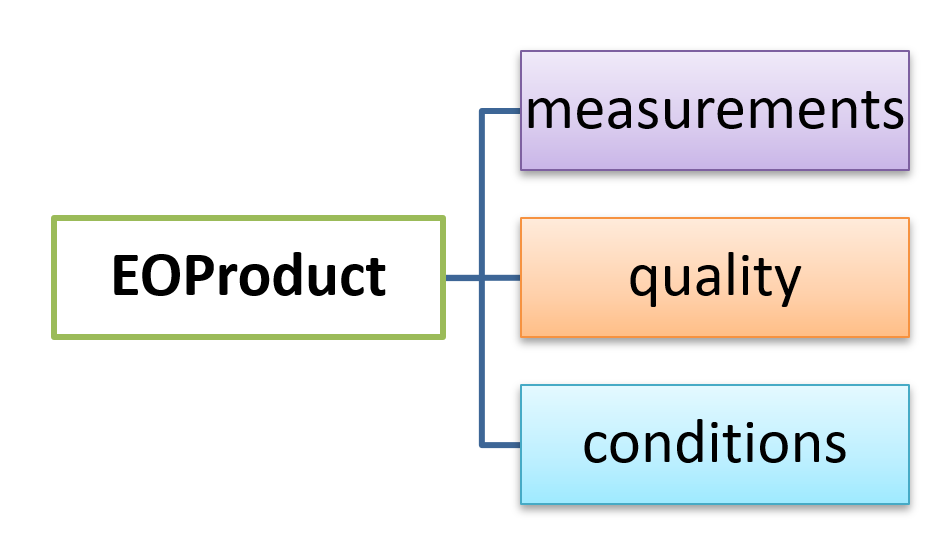
\includegraphics[keepaspectratio]{img/EOProduct-structure.png}}

}

\caption{EOPF product structure}

\end{figure}%

\begin{tcolorbox}[enhanced jigsaw, coltitle=black, colback=white, leftrule=.75mm, colbacktitle=quarto-callout-note-color!10!white, titlerule=0mm, title=\textcolor{quarto-callout-note-color}{\faInfo}\hspace{0.5em}{Note}, rightrule=.15mm, bottomrule=.15mm, bottomtitle=1mm, toptitle=1mm, arc=.35mm, toprule=.15mm, left=2mm, opacityback=0, colframe=quarto-callout-note-color-frame, opacitybacktitle=0.6, breakable]

Learn more about the EOPF Zarr product structure
\href{./21_what_is_zarr.qmd}{here}.

\end{tcolorbox}

\subsection{EOPF metadata structure}\label{eopf-metadata-structure}

Metadata provide all relevant information required to uniquely
describing each Sentinel product. The EOPF metadata structure is
organised as follows:

\begin{itemize}
\tightlist
\item
  \textbf{Discovery Metadata}: Following the metadata structure defined
  by the SpatioTemporal Asset Catalogue
  (\href{https://stacspec.org/en/}{STAC}), which helps to keep things
  consistent across different missions.
\item
  \textbf{Processing History Metadata}: Keeping a record of how the data
  has been processed.
\item
  \textbf{Other Metadata}: Information like the status of the sensor and
  details about the satellite's orbit.
\end{itemize}

\begin{tcolorbox}[enhanced jigsaw, coltitle=black, colback=white, leftrule=.75mm, colbacktitle=quarto-callout-note-color!10!white, titlerule=0mm, title=\textcolor{quarto-callout-note-color}{\faInfo}\hspace{0.5em}{Note}, rightrule=.15mm, bottomrule=.15mm, bottomtitle=1mm, toptitle=1mm, arc=.35mm, toprule=.15mm, left=2mm, opacityback=0, colframe=quarto-callout-note-color-frame, opacitybacktitle=0.6, breakable]

EOPF and STAC: Learn more about EOPF and STAC
\href{./31_stac_intro.qmd}{here}.

\end{tcolorbox}

\subsection{EOPF encoding structure}\label{eopf-encoding-structure}

An encoding structure can be seen as the specific method used to package
and store data and its associated metadata in a digital format. Building
on the consistent data structure and clear metadata, the new storage
system must be capable of handling various aspects of current Sentinel
data (such as manifest files and tile structures from the SAFE format)
while remaining fully compatible with cloud environments.

ESA chose \texttt{.zarr} as encoding format as it allows for instant
access to data, efficient processing of massive amounts of data, and
seamless integration with other datasets. The EOPF Sentinel Zarr data
encoding allows you to work with data from multiple missions more
effectively.

\begin{tcolorbox}[enhanced jigsaw, coltitle=black, colback=white, leftrule=.75mm, colbacktitle=quarto-callout-note-color!10!white, titlerule=0mm, title=\textcolor{quarto-callout-note-color}{\faInfo}\hspace{0.5em}{Note}, rightrule=.15mm, bottomrule=.15mm, bottomtitle=1mm, toptitle=1mm, arc=.35mm, toprule=.15mm, left=2mm, opacityback=0, colframe=quarto-callout-note-color-frame, opacitybacktitle=0.6, breakable]

Learn more about the EOPF Sentinel Zarr format
\href{https://zarr.eopf.copernicus.eu/}{here}. And learn more about
cloud-optimised geospatial data formats in general in the
\href{https://guide.cloudnativegeo.org/}{Cloud-Optimised Geospatial Data
Formats Guide}

\end{tcolorbox}

\subsection{EOPF processor framework}\label{eopf-processor-framework}

The way Sentinel data is processed is being updated to take advantage of
modern cloud computing. This will make the processing faster and more
efficient and at the same time ensuring the scientific quality and
accuracy of the Sentinel data remains the same.

\begin{tcolorbox}[enhanced jigsaw, coltitle=black, colback=white, leftrule=.75mm, colbacktitle=quarto-callout-note-color!10!white, titlerule=0mm, title=\textcolor{quarto-callout-note-color}{\faInfo}\hspace{0.5em}{Note}, rightrule=.15mm, bottomrule=.15mm, bottomtitle=1mm, toptitle=1mm, arc=.35mm, toprule=.15mm, left=2mm, opacityback=0, colframe=quarto-callout-note-color-frame, opacitybacktitle=0.6, breakable]

To learn more about the EOPF processor framework, visit
\url{https://eopf.copernicus.eu/eopf/}

\end{tcolorbox}

\section{Conclusion}\label{conclusion}

Throughout this section, we explored the EOPF initiative and its
adoption of the \texttt{.zarr}format. This new approach is set to
significantly improve and simplify how we access and work with data the
satellite mission Sentinel-1, Sentinel-2, and Sentinel-3.

\section{What's next?}\label{whats-next}

In the following \href{./12_about_cloudoptimized_formats.qmd}{section},
we learn why EO data need to be cloud-optimised, when processed in the
cloud.

\chapter{About cloud-optimised
formats}\label{about-cloud-optimised-formats}

\subsection{Introduction}\label{introduction-1}

In this section, we will dive into \textbf{cloud-optimised geospatial
formats}. We explore why these new formats are important and will
introduce you two common cloud-optimised data formats specifcially for
raster files.

\subsection{What we will learn}\label{what-we-will-learn}

\begin{itemize}
\tightlist
\item
  ☁️ What do we need to cloud-optimise geospatial data?
\item
  🏛️ Differences between traditional and cloud-native workflows
\item
  📖 What are the main characteristics of cloud-optimised formats?
\item
  💾 What are \textbf{COGs} and \textbf{Zarr}, and how do they differ?
\end{itemize}

\section{Why to cloud-optimise geospatial data
formats?}\label{why-to-cloud-optimise-geospatial-data-formats}

The volume of EO data has grown exponentially in recent years. The
Copernicus programme alone generates \textasciitilde16TB daily from the
Sentinel missions. Traditional file formats, like SAFE (where each file
can be hundreds of megabytes), are optimised for efficient archiving and
distributing data. This means that we often download the data from an
entire overpass, even if we only need to access a small part of it. For
example, if we want to do an analysis of the area of a single city over
a decade.

With growing data volumes, this becomes a challenge. To picture the
different nature of challenges we come across, let us compare a
traditional local workflow with a cloud-based workflow:

\begin{itemize}
\item
  \textbf{Traditional local workflow}: When working locally, we download
  much more data than we need, and we are constrained by the compute and
  storage capacity of the local system. However, an advantage working
  locally is that data and compute are close together, meaning that
  there is not much delay in accessing the data.
\item
  \textbf{Cloud-based workflow}: Cloud environments overcome limitations
  local workflows have. A cloud environment offers limitless storage and
  compute capacity. On the contrary, data storage, compute, and you the
  destination are far apart. There is an additional time for data to
  travel between the storage location, processing resources and us. This
  time is referred to as \textbf{data latency}.
\end{itemize}

\begin{tcolorbox}[enhanced jigsaw, coltitle=black, colback=white, leftrule=.75mm, colbacktitle=quarto-callout-note-color!10!white, titlerule=0mm, title=\textcolor{quarto-callout-note-color}{\faInfo}\hspace{0.5em}{Note}, rightrule=.15mm, bottomrule=.15mm, bottomtitle=1mm, toptitle=1mm, arc=.35mm, toprule=.15mm, left=2mm, opacityback=0, colframe=quarto-callout-note-color-frame, opacitybacktitle=0.6, breakable]

\textbf{Data latency} refers to the time it takes for data to be
transmitted or processed from cloud storage to your computer. In local
workflows, data latency is minimal, whereas in cloud-based workflows,
data latency needs to be optimised.

\end{tcolorbox}

\subsection{Analogy: Comparing local and cloud-based workflows with
ordering a
pizza}\label{analogy-comparing-local-and-cloud-based-workflows-with-ordering-a-pizza}

To understand the principal concept, let us compare local and
cloud-based workflows with ordering a pizza. Local workflows are similar
to placing an order a pizza store in your street. It is quick since the
`data' (pizza) is easily accessible, but we can only choose from what
the local pizza store offers.

On the other hand, cloud-based workflows are comparable to ordering a
pizza from a pizza store in a different city or even country. This
option allows you to order different types of pizzas, which are not
available in pizza store in your street. While we might have more
options to choose from, the time between order and delivery can become a
challenge. The time until your pizza from a different town or country
arrives at your house is called \textbf{data latency}.

Hence, the overall goal with cloud-based workflows is to minimise
\textbf{data latency} as much as possible. This is why traditional data
formats need to be cloud-optimised.

\section{Characteristics of cloud-optimised
formats}\label{characteristics-of-cloud-optimised-formats}

Cloud-optimised formats are optimised to minimise data latency. By
allowing for an efficient retrieval of smaller, specific chunks of
information rather than downloading an entire file. Accessing a smaller
data subset also reduces the costs associated with data transfer and
data processing.

Cloud-optimised geospatial data formats have the following
characteristics:

\begin{itemize}
\tightlist
\item
  Data is \textbf{accessible over an HTTP protocol}.
\item
  \textbf{Read-Oriented}, as it supports partial and parallel reads.
\item
  Data is \textbf{organised in internal groupings (such as chunks,
  tiles, shards)} for efficient subsetting, distributed processing and
  data access in memory.
\item
  \textbf{Metadata} can be accessed in one read.
\end{itemize}

\begin{tcolorbox}[enhanced jigsaw, coltitle=black, colback=white, leftrule=.75mm, colbacktitle=quarto-callout-note-color!10!white, titlerule=0mm, title=\textcolor{quarto-callout-note-color}{\faInfo}\hspace{0.5em}{Note}, rightrule=.15mm, bottomrule=.15mm, bottomtitle=1mm, toptitle=1mm, arc=.35mm, toprule=.15mm, left=2mm, opacityback=0, colframe=quarto-callout-note-color-frame, opacitybacktitle=0.6, breakable]

When accessing data over the internet (e.g.~through object stores in the
cloud), latency is high compared to local storage, so it is recommended
to fetch lots of data in fewer reads.

\end{tcolorbox}

\section{Cloud-Optimised Geospatial Raster
Formats}\label{cloud-optimised-geospatial-raster-formats}

For satellite data, there are two main cloud-optimised formats being
used: - \textbf{Cloud-Optimized GeoTIFF (COG)}: Optimized for 2D image
data and originates from the traditional \texttt{GeoTIFF} format, and -
\textbf{Zarr}: Used and designed for complex, n-dimensional data
structures and originates from the traditional formats \texttt{netCDF}
and \texttt{HDF5}.

\subsection{Cloud-optimised GeoTIFF
(COG)}\label{cloud-optimised-geotiff-cog}

COGs have widely been used as cloud-native format for satellite imagery
and improve the standard GeoTIFF format by: - Organising data into
\textbf{tiles}: Dividing the data into smaller, manageable squares (like
512x512 pixels). - Including lower-resolution previews: Having
pre-generated, less detailed versions of the data. This allows for fast
and efficient data visualisations.

A key feature of COGs is the \textbf{Internal File Directory} (IFD),
which acts like an internal index. This allows for retrieving only the
parts of the data needed using simple web requests. For example, it is
possible to access just the tiles covering Paris from a large Sentinel-2
image of Europe.

\begin{figure}[H]

{\centering \pandocbounded{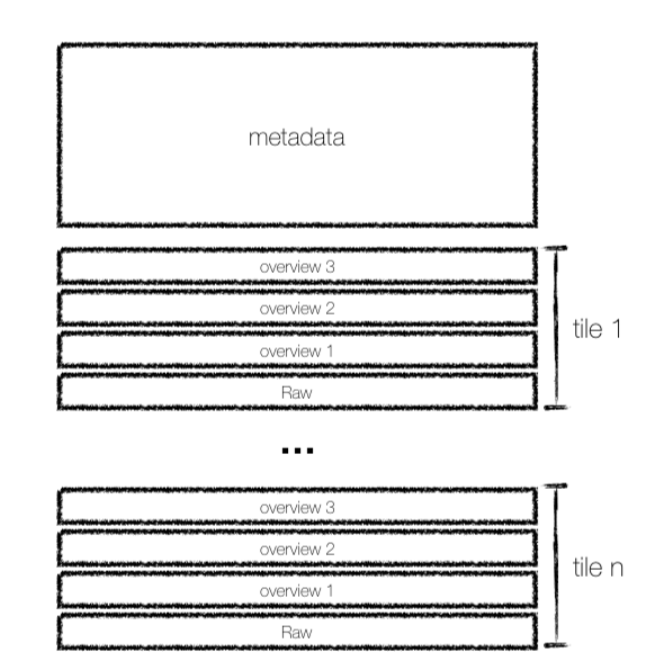
\includegraphics[keepaspectratio]{img/cogtiff.png}}

}

\caption{COG structure. Retrieved from CNG documentation}

\end{figure}%

\subsection{Multi-dimensional Array Storage with
Zarr}\label{multi-dimensional-array-storage-with-zarr}

Zarr is the cloud-optimised version for the traditional formats
\texttt{netCDF} and \texttt{HDF5} and is specifically designed for
storing and accessing large n-dimensional arrays in the cloud by:

\begin{itemize}
\tightlist
\item
  \textbf{Chunking}: Breaking large arrays into smaller pieces that can
  be accessed independently
\item
  \textbf{Compression}: Each chunk can be compressed individually for
  efficient storage
\item
  \textbf{Hierarchical Organization}: Arrays are organized in groups,
  similar to folders in a filesystem
\item
  \textbf{Cloud-Native Access}: Optimized for reading partial data over
  HTTP
\item
  \textbf{Parallel I/O}: Multiple chunks can be read or written
  simultaneously
\item
  \textbf{Self-Description}: Rich metadata is stored alongside the data
  using JSON
\end{itemize}

This makes Zarr particularly well-suited as storage format for
processing Earth observation data in the cloud.

\begin{figure}[H]

{\centering \pandocbounded{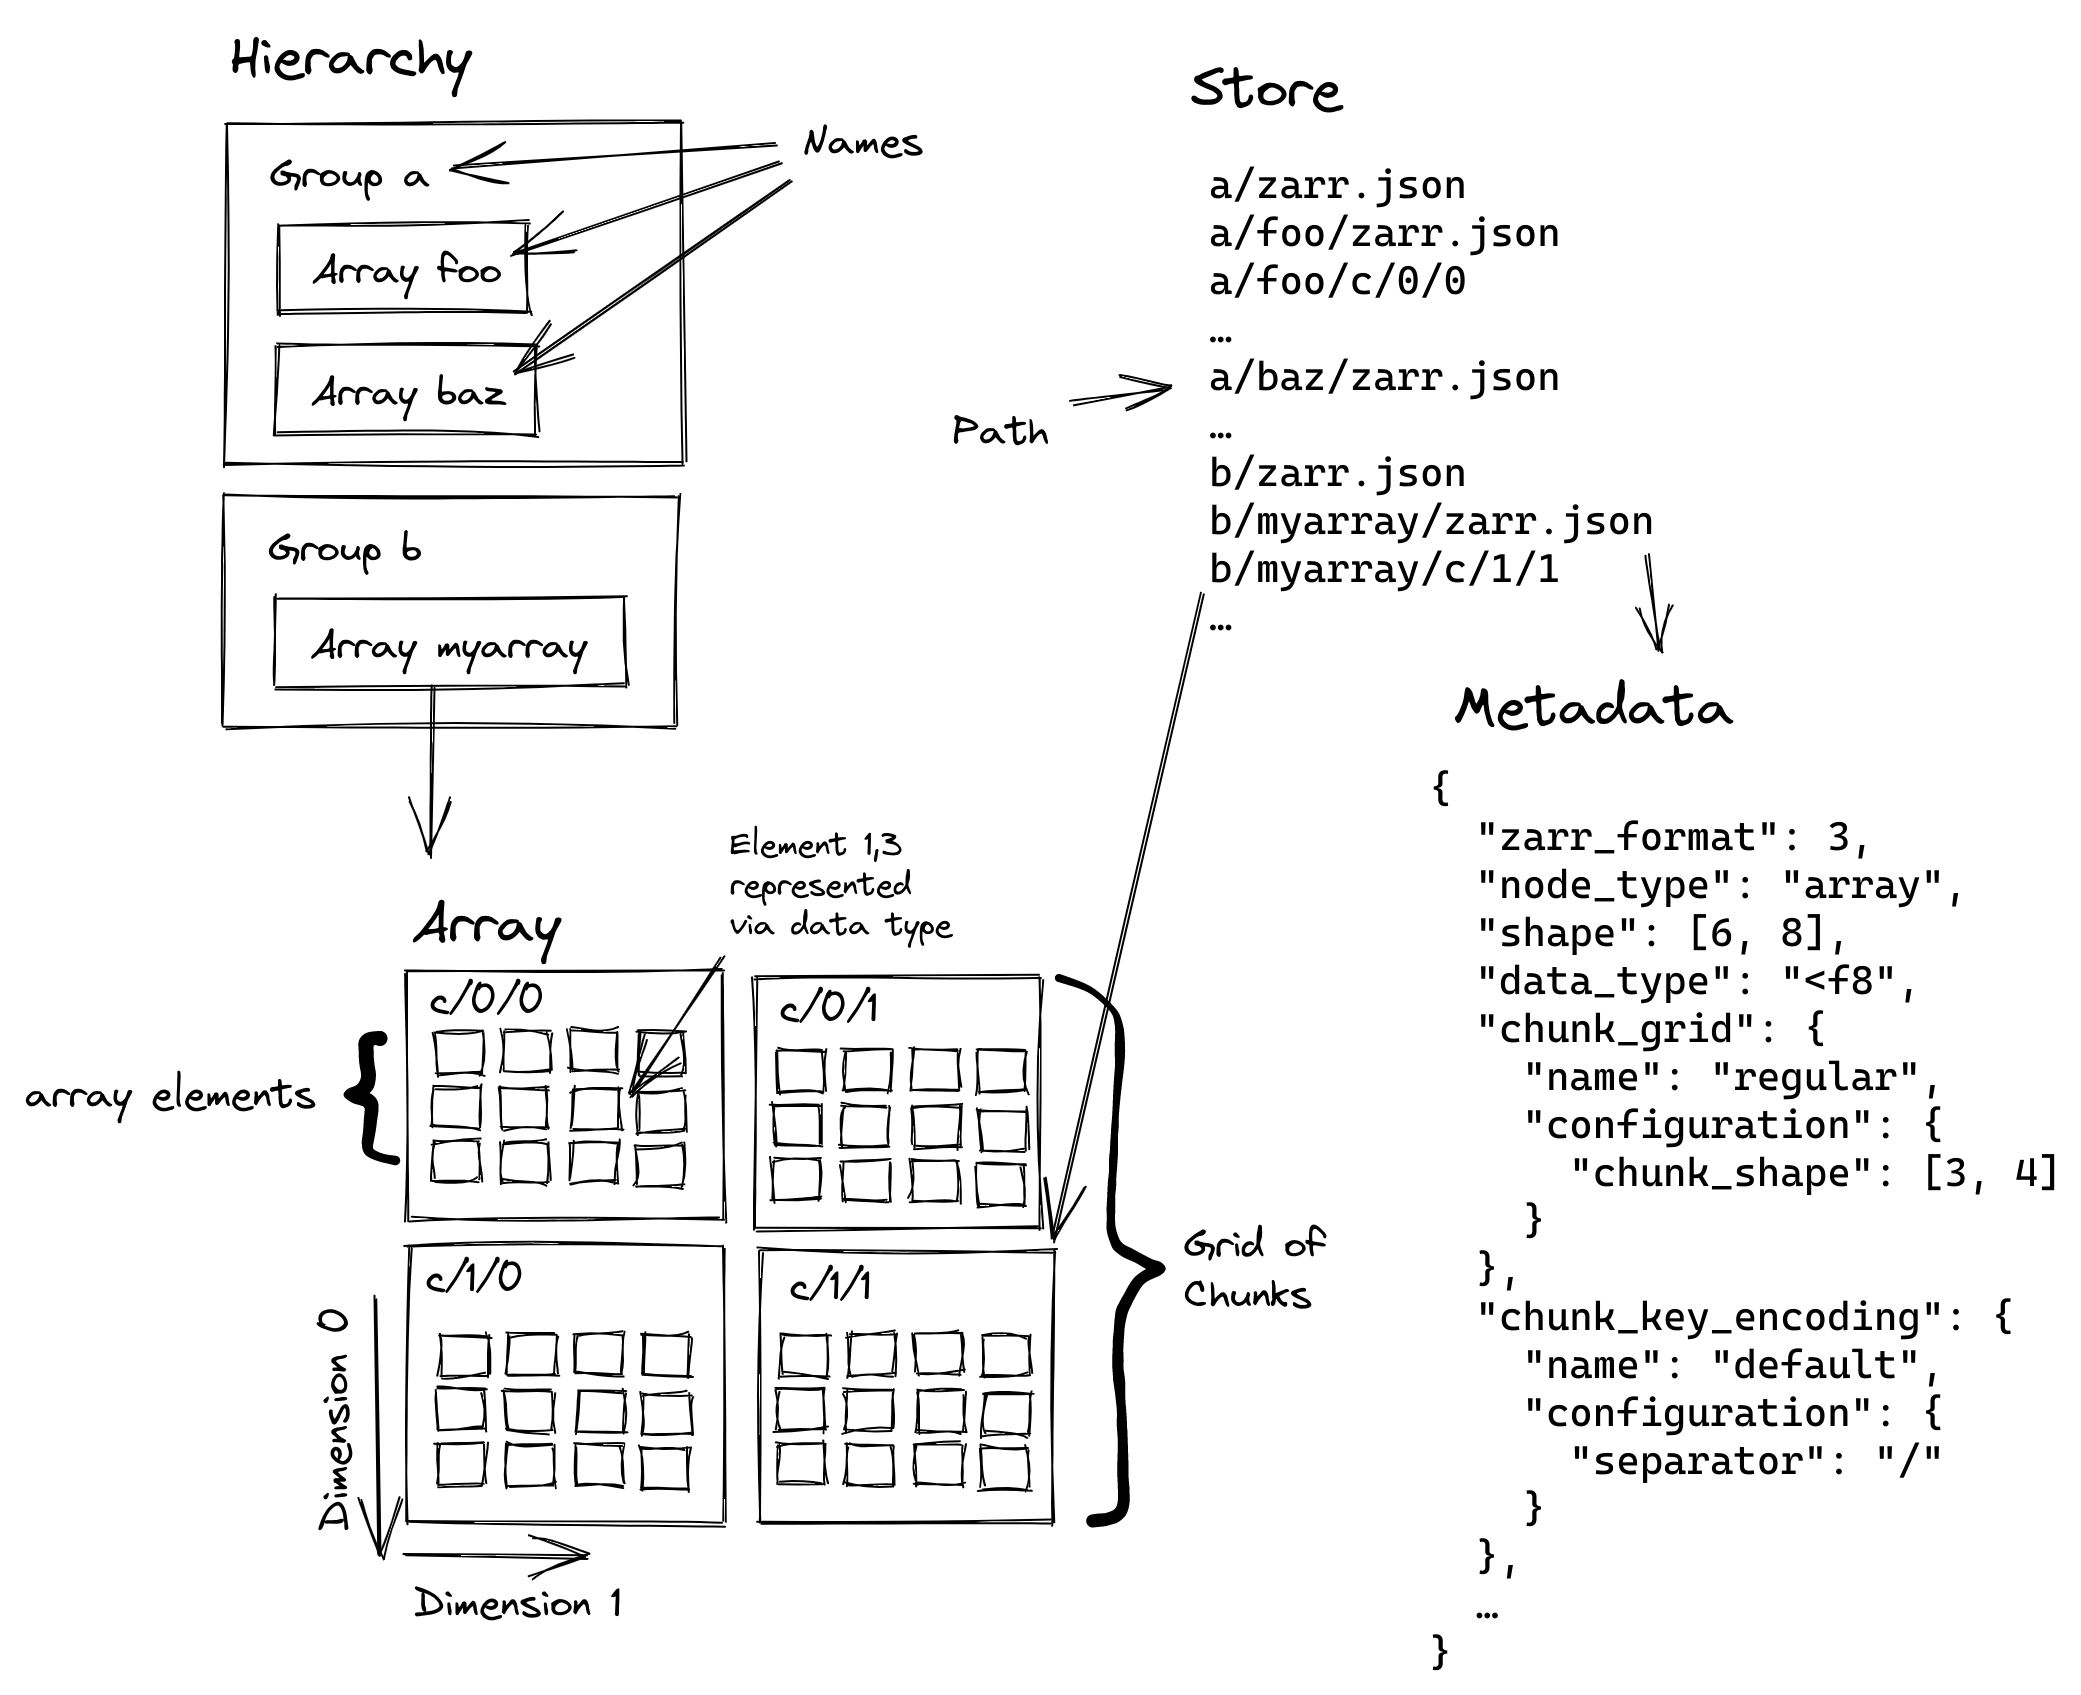
\includegraphics[keepaspectratio]{img/zarr-terminology-hierarchy.png}}

}

\caption{Zarr's hierarchical organization showing stores, groups,
arrays, and chunks}

\end{figure}%

\subsection{When to use COG versus
Zarr?}\label{when-to-use-cog-versus-zarr}

The table below compares some features of COG and Zarr:

\begin{longtable}[]{@{}
  >{\raggedright\arraybackslash}p{(\linewidth - 4\tabcolsep) * \real{0.2500}}
  >{\raggedright\arraybackslash}p{(\linewidth - 4\tabcolsep) * \real{0.3750}}
  >{\raggedright\arraybackslash}p{(\linewidth - 4\tabcolsep) * \real{0.3750}}@{}}
\toprule\noalign{}
\begin{minipage}[b]{\linewidth}\raggedright
Feature
\end{minipage} & \begin{minipage}[b]{\linewidth}\raggedright
Zarr
\end{minipage} & \begin{minipage}[b]{\linewidth}\raggedright
COG
\end{minipage} \\
\midrule\noalign{}
\endhead
\bottomrule\noalign{}
\endlastfoot
Structure & Multi-file chunks & Single file \\
Access & Parallel & Sequential \\
Compression & Differently per-chunk & Whole-file \\
Scales & Multi-scale in single file & Separate, pre-generated
lower-resolution files \\
\end{longtable}

Based on the structure and capabilities for each format, \textbf{COGs}
are used when:

\begin{itemize}
\tightlist
\item
  you work with two-dimensional raster data (like satelliteimages or
  elevation models)
\item
  you need to easily visualise or access specific geographic areas
  without loading the entire dataset.
\item
  interoperability with existing GIS software is important, as COG is a
  widely adopted standard.
\end{itemize}

On the other hand, \textbf{Zarr} is more often used when:

\begin{itemize}
\tightlist
\item
  you deal with large, multi-dimensional datasets that might be updated
  or modified.
\item
  you performing complex analyses that involve accessing different parts
  of the data in parallel.
\item
  an efficient handling of different resolutions or variables within a
  single dataset is required.
\end{itemize}

\begin{tcolorbox}[enhanced jigsaw, coltitle=black, colback=white, leftrule=.75mm, colbacktitle=quarto-callout-note-color!10!white, titlerule=0mm, title=\textcolor{quarto-callout-note-color}{\faInfo}\hspace{0.5em}{Note}, rightrule=.15mm, bottomrule=.15mm, bottomtitle=1mm, toptitle=1mm, arc=.35mm, toprule=.15mm, left=2mm, opacityback=0, colframe=quarto-callout-note-color-frame, opacitybacktitle=0.6, breakable]

Zarr vs COG: Want to learn more about the differences and similarities
of COG and Zarr? Then we recommend the following blog post by Julia
Signell and Jarrett Keifer from Element84 where they discuss
``\href{https://element84.com/software-engineering/is-zarr-the-new-cog/}{Is
Zarr the new COG?}''

\end{tcolorbox}

\section{Conclusion}\label{conclusion-1}

In this section, we explored the fundamental concepts of
\textbf{cloud-optimised geospatial formats}. By understanding the core
characteristics of these formats and by looking at specific examples
like \textbf{Zarr}, you now have a solid foundation for appreciating how
these innovations are making geospatial data more accessible, efficient,
and powerful in the cloud.

\section{What's next?}\label{whats-next-1}

Now that we have an idea of the available cloud-optimised formats for
satellite imagery and the reason why we need to optimise traditional
formats for the cloud, in the next
\href{./13_overview_eopf_datasets.qmd}{section}, we will explore the
EOPF data products that are being re-processed as part of the EOPF Zarr
Sample Service.

\chapter{Overview of EOPF Zarr
Products}\label{overview-of-eopf-zarr-products}

\subsection{Introduction}\label{introduction-2}

In previous section, we introduced the \textbf{Earth Observation
Processing Framework} (EOPF) initiative and explored the advantages of
cloud-optimised formats like Zarr. Now, it is time to discover which
data products will be available and where you can access those.

\subsection{What we will learn}\label{what-we-will-learn-1}

\begin{itemize}
\tightlist
\item
  💾 What Sentinel data will be available as EOPF Zarr products?
\item
  🛰️ A sneak-peak into where you can access EOPF Zarr products
\end{itemize}

\section{Available EOPF Zarr
products}\label{available-eopf-zarr-products}

Re-engineered EOPF Zarr products are available for exploration via the
\href{https://stac.browser.user.eopf.eodc.eu/?.language=en}{EOPF
Sentinel Zarr Sample Service STAC Catalog}. Data from Sentinel-1,
Sentinel-2 and Sentinel-3 missions are being re-processed and made
available.

\begin{tcolorbox}[enhanced jigsaw, coltitle=black, colback=white, leftrule=.75mm, colbacktitle=quarto-callout-important-color!10!white, titlerule=0mm, title=\textcolor{quarto-callout-important-color}{\faExclamation}\hspace{0.5em}{Important}, rightrule=.15mm, bottomrule=.15mm, bottomtitle=1mm, toptitle=1mm, arc=.35mm, toprule=.15mm, left=2mm, opacityback=0, colframe=quarto-callout-important-color-frame, opacitybacktitle=0.6, breakable]

The re-processing from the Sentinel missions is an ongoing activity as
part of the \href{https://zarr.eopf.copernicus.eu/}{EOPF Sentinel Zarr
Sample Service}. This page and our tutorials will continuously be
updated as soon as new data products are available.

\end{tcolorbox}

An overview of the datasets that are being re-engineered for different
processing levels is given below.

\subsection{Sentinel-1}\label{sentinel-1}

Sentinel-1 is a radar imaging mission that is composed of a
constellation of two polar-orbiting satellites providing continuous
all-weather, day and night imagery.

\begin{longtable}[]{@{}
  >{\raggedright\arraybackslash}p{(\linewidth - 6\tabcolsep) * \real{0.2500}}
  >{\raggedright\arraybackslash}p{(\linewidth - 6\tabcolsep) * \real{0.2500}}
  >{\raggedright\arraybackslash}p{(\linewidth - 6\tabcolsep) * \real{0.2500}}
  >{\raggedright\arraybackslash}p{(\linewidth - 6\tabcolsep) * \real{0.2500}}@{}}
\toprule\noalign{}
\begin{minipage}[b]{\linewidth}\raggedright
Product
\end{minipage} & \begin{minipage}[b]{\linewidth}\raggedright
Instrument
\end{minipage} & \begin{minipage}[b]{\linewidth}\raggedright
Description
\end{minipage} & \begin{minipage}[b]{\linewidth}\raggedright
Available at
\end{minipage} \\
\midrule\noalign{}
\endhead
\bottomrule\noalign{}
\endlastfoot
Level-1 GRD & Ground Range Detected & The Sentinel-1 Level-1 GDR
products consist of focused SAR data that has been detected,
multi-looked and projected to ground range using the Earth ellipsoid
model WGS84. &
\href{https://stac.browser.user.eopf.eodc.eu/collections/sentinel-1-l1-grd?.language=en}{this
link} \\
Level-1 SLC & Single Look Complex ( & The Sentinel-1 Level-1 SLC
products consist of focused SAR data, geo-referenced using orbit and
attitude data from the satellite, and provided in slant-range geometry.
&
\href{https://stac.browser.user.eopf.eodc.eu/collections/sentinel-1-l1-slc?.language=en}{this
link} \\
Level-2 OCN & Ocean & The Sentinel-1 Level-2 OCN products for wind, wave
and currents applications may contain the following geophysical
components derived from the SAR data: Ocean Wind field (OWI), Ocean
Swell spectra (OSW), Surface Radial Velocity (RVL). &
\href{https://stac.browser.user.eopf.eodc.eu/collections/sentinel-1-l2-ocn?.language=en}{this
link} \\
\end{longtable}

\subsection{Sentinel-2}\label{sentinel-2}

Sentinel-2 acquires optical imagery at high spatial resolution (10m to
60m) over land and coastal waters. The mission supports applications
such as agricultural monitoring, emergency management, land cover
classifications, and water quality.

\begin{longtable}[]{@{}
  >{\raggedright\arraybackslash}p{(\linewidth - 6\tabcolsep) * \real{0.2500}}
  >{\raggedright\arraybackslash}p{(\linewidth - 6\tabcolsep) * \real{0.2500}}
  >{\raggedright\arraybackslash}p{(\linewidth - 6\tabcolsep) * \real{0.2500}}
  >{\raggedright\arraybackslash}p{(\linewidth - 6\tabcolsep) * \real{0.2500}}@{}}
\toprule\noalign{}
\begin{minipage}[b]{\linewidth}\raggedright
Product
\end{minipage} & \begin{minipage}[b]{\linewidth}\raggedright
Instrument
\end{minipage} & \begin{minipage}[b]{\linewidth}\raggedright
Description
\end{minipage} & \begin{minipage}[b]{\linewidth}\raggedright
Available at
\end{minipage} \\
\midrule\noalign{}
\endhead
\bottomrule\noalign{}
\endlastfoot
Level-1C & Multi-Spectral Instrument & The Sentinel-2 Level-1C product
is composed of 110x110 km2 tiles (ortho-images in UTM/WGS84 projection).
Earth is subdivided on a predefined set of tiles, defined in UTM/WGS84
projection and using a 100 km step. &
\href{https://stac.browser.user.eopf.eodc.eu/collections/sentinel-2-l1c}{this
link} \\
Level-2A & Multi-Spectral Instrument & The Sentinel-2 Level-2A
Collection 1 product provides orthorectified Surface Reflectance
(Bottom-Of-Atmosphere: BOA), with sub-pixel multispectral and
multitemporal registration accuracy. &
\href{https://stac.browser.user.eopf.eodc.eu/collections/sentinel-2-l2a}{this
link} \\
\end{longtable}

\subsection{Sentinel-3}\label{sentinel-3}

Sentinel-3 is a mission that regularly measures our Earth's oceans,
land, rivers, lakes, ice on land, sea ice, and the atmosphere. Its goal
is to keep track of and help us understand how these large parts of our
planet change over long periods.

\subsubsection{Ocean and Land Colour
Instrument}\label{ocean-and-land-colour-instrument}

\begin{longtable}[]{@{}
  >{\raggedright\arraybackslash}p{(\linewidth - 6\tabcolsep) * \real{0.2500}}
  >{\raggedright\arraybackslash}p{(\linewidth - 6\tabcolsep) * \real{0.2500}}
  >{\raggedright\arraybackslash}p{(\linewidth - 6\tabcolsep) * \real{0.2500}}
  >{\raggedright\arraybackslash}p{(\linewidth - 6\tabcolsep) * \real{0.2500}}@{}}
\toprule\noalign{}
\begin{minipage}[b]{\linewidth}\raggedright
Product
\end{minipage} & \begin{minipage}[b]{\linewidth}\raggedright
Product
\end{minipage} & \begin{minipage}[b]{\linewidth}\raggedright
Description
\end{minipage} & \begin{minipage}[b]{\linewidth}\raggedright
Available at
\end{minipage} \\
\midrule\noalign{}
\endhead
\bottomrule\noalign{}
\endlastfoot
Level-1 EFR & Earth Full Resolution & Provides TOA radiances at full
resolution for each pixel in the instrument grid, each view and each
OLCI channel, plus annotation data associated to OLCI pixels. &
\href{https://stac.browser.user.eopf.eodc.eu/collections/sentinel-3-olci-l1-efr}{this
link} \\
Level-1 ERR & Earth Reduced Resolution & The Sentinel-3 OLCI L1 ERR
product provides TOA radiances at reduced resolution for each pixel in
the instrument grid, each view and each OLCI channel, plus annotation
data associated to OLCI pixels. &
\href{https://stac.browser.user.eopf.eodc.eu/collections/sentinel-3-olci-l1-err}{this
link} \\
Level-2 LFR & Land Full Resolution & The Sentinel-3 OLCI L2 LFR product
provides land and atmospheric geophysical parameters computed for full
resolution. &
\href{https://stac.browser.user.eopf.eodc.eu/collections/sentinel-3-olci-l2-lfr}{this
link} \\
Level-2 LRR & Land Reduced Resolution & The Sentinel-3 OLCI L2 LRR
product provides land and atmospheric geophysical parameters computed
for reduced resolution. &
\href{https://stac.browser.user.eopf.eodc.eu/collections/sentinel-3-olci-l2-lrr}{this
link} \\
\end{longtable}

\subsubsection{Sea and Land Surface Temperature
Radiometer}\label{sea-and-land-surface-temperature-radiometer}

\begin{longtable}[]{@{}
  >{\raggedright\arraybackslash}p{(\linewidth - 6\tabcolsep) * \real{0.2500}}
  >{\raggedright\arraybackslash}p{(\linewidth - 6\tabcolsep) * \real{0.2500}}
  >{\raggedright\arraybackslash}p{(\linewidth - 6\tabcolsep) * \real{0.2500}}
  >{\raggedright\arraybackslash}p{(\linewidth - 6\tabcolsep) * \real{0.2500}}@{}}
\toprule\noalign{}
\begin{minipage}[b]{\linewidth}\raggedright
Product
\end{minipage} & \begin{minipage}[b]{\linewidth}\raggedright
Data
\end{minipage} & \begin{minipage}[b]{\linewidth}\raggedright
Description
\end{minipage} & \begin{minipage}[b]{\linewidth}\raggedright
Available at
\end{minipage} \\
\midrule\noalign{}
\endhead
\bottomrule\noalign{}
\endlastfoot
Level-1 RBT & Radiance Brightness Temperature & The Sentinel-3 SLSTR
Level-1B RBT product provides radiances and brightness temperatures for
each pixel in a regular image grid for each view and SLSTR channel. &
\href{https://stac.browser.user.eopf.eodc.eu/collections/sentinel-3-slstr-l1-rbt}{this
link} \\
Level-2 LST & LST: Land Surface Temperature & The Sentinel-3 SLSTR
Level-2 LST product provides land surface temperature. &
\href{https://stac.browser.user.eopf.eodc.eu/collections/sentinel-3-slstr-l2-lst}{this
link} \\
\end{longtable}

\section{Conclusion}\label{conclusion-2}

In this section we provide an overview of the the available
\textbf{Sentinel Missions} that will be re-processed and made available
as EOPF Zarr products.

\section{What's next?}\label{whats-next-2}

In the following \href{21_what_is_zarr.qmd}{chapter}, we will dive deep
into \texttt{EOPF\ Zarr} format and understand why it can provide an
optimal and efficient application.

\part{\textbf{About EOPF Zarr}}

\chapter{Overview of the EOPF Zarr
format}\label{overview-of-the-eopf-zarr-format}

\subsection{Introduction}\label{introduction-3}

In our journey to understand \textbf{cloud-optimised Earth Observation}
(EO) data, we have frequently mentioned the \textbf{Zarr} format. Now,
we will take a closer look and truly understand what \textbf{Zarr} is
and why it is such a game-changer for large datasets like those from
ESA's Sentinel missions. This chapter will break down the essential
building blocks of \textbf{Zarr}, explaining how it organises data to
make it incredibly efficient for cloud-based analysis.

\subsection{What we will learn}\label{what-we-will-learn-2}

\begin{itemize}
\tightlist
\item
  🔗 What is Zarr?
\item
  🏛️ What are the main components of Zarr?
\item
  🧱 How is Zarr organised?
\end{itemize}

\section{What Is Zarr?}\label{what-is-zarr}

\textbf{Zarr} is an open-source, cloud-native protocol for storing
multi-dimensional arrays. It is specifically desgined to work well with
cloud storage and larger-scale computing systems and can be seen as a
cloud-native alternative to older formats like HDF5 or NetCDF.

Key advantage to traditional formats is that the Zarr specification
stores large multi-dimensional arrays in \textbf{chunks}, which are
smaller pieces of the larger array. Chunks can be accessed individually
or multiple chunks can be read and written in parallel, making data
access highly \textbf{efficient}.

Zarr works across different storage systems, including local file
systems, cloud object storage as well as distributed file systems;
offering a greater \textbf{flexibility} compared to traditional file
formats.

In addition, Zarr embeds \textbf{metadata} directly alongside the data.
This makes Zarr \textbf{self-descriptive}, as each data array contains
descriptive information about itself, such as data type, dimensions or
additional attributes.

\begin{tcolorbox}[enhanced jigsaw, coltitle=black, colback=white, leftrule=.75mm, colbacktitle=quarto-callout-note-color!10!white, titlerule=0mm, title=\textcolor{quarto-callout-note-color}{\faInfo}\hspace{0.5em}{Note}, rightrule=.15mm, bottomrule=.15mm, bottomtitle=1mm, toptitle=1mm, arc=.35mm, toprule=.15mm, left=2mm, opacityback=0, colframe=quarto-callout-note-color-frame, opacitybacktitle=0.6, breakable]

Pro tip: Learn more about Zarr in the official
\href{https://zarr.dev/}{Zarr Documentation} and the
\href{https://zarr-specs.readthedocs.io/en/latest/v3/core/index.html}{Zarr
V3 storage specification}

\end{tcolorbox}

\section{Components of Zarr}\label{components-of-zarr}

Zarr is organised in a \textbf{human-readable}, \textbf{hierarchical}
structure using simple JSON metadata files and is composed of
\texttt{groups\ and\ stores}, \texttt{chunks} and \texttt{metadata}:

\subsection{Groups and Stores}\label{groups-and-stores}

\textbf{Groups} and \textbf{stores} are concepts that allow Zarr to
differentiate between (i) where the data is stored (\textbf{stores}) and
(ii) how it is organised (\textbf{groups}). A \textbf{group} is a
container for logically organising the data, similar to folders in a
file system. A \textbf{store} defines where the data is stored; it can
be e.g.~a bucket in the cloud or a directory on a disk.

\subsection{Chunks}\label{chunks}

Zarr divides arrays into smaller, independent pieces (\textbf{chunks}).
Through chunking it is possible to retrieve and process specific areas
without loading the complete dataset. Its organisation into chunks is
the main reason Zarr's high performance. Chunks are saved as binary
files inside a \texttt{/c} directory and are further organised through
nested folder paths based on their index, e.g.~\texttt{c/0/0/0} for the
chunk position \texttt{{[}0,0.0{]}}.

\subsection{Metadata}\label{metadata}

Zarr uses descriptive \textbf{metadata} to describe the individual
arrays but also the full hierarchy of the dataset. Metadata are stored
in \texttt{zarr.json} files and are available on the array, group and
store level. This structured metadata approach makes Zarr datasets
\textbf{self-descriptive} and easy to navigate.

The graphic below shows an overview of all relevant Zarr components.

\begin{figure}[H]

{\centering \pandocbounded{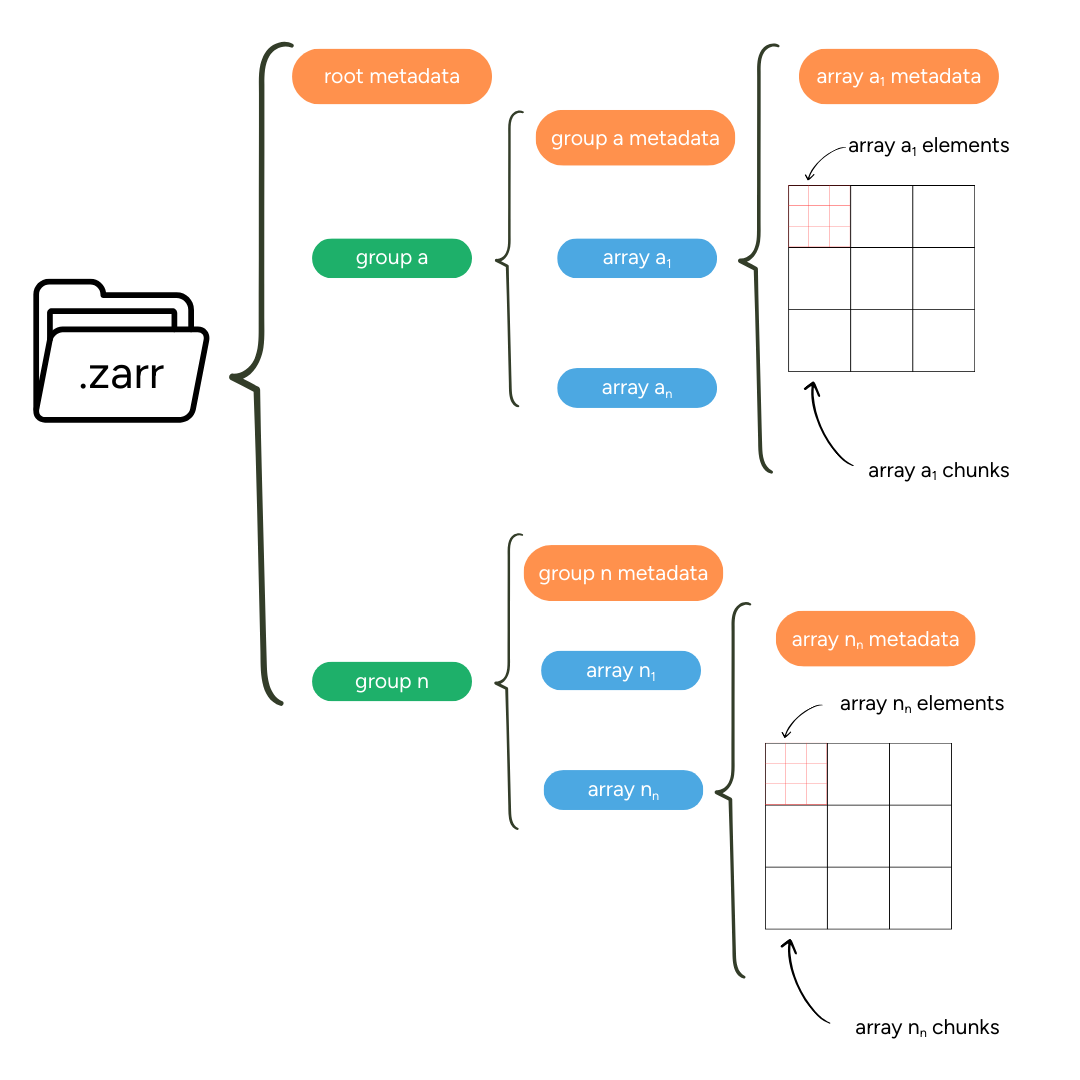
\includegraphics[keepaspectratio]{img/zarr_str.png}}

}

\caption{Zarr conceptual structure and overview of Zarr components}

\end{figure}%

\section{EOPF Zarr Structure}\label{eopf-zarr-structure}

The ESA EOPF defines \texttt{Zarr} as the encoding format for the
\href{https://zarr.eopf.copernicus.eu/}{EOPF Sentinel Zarr Samples
Service}. The Zarr encoding is well aligned with ESA's objective of
enhancing the accessibility of Sentinel data by modernising the previous
\texttt{.SAFE} encoding into a flexible, cloud-native structure. The
cloud-native nature of \texttt{zarr} is expected to broaden the
applications of the Sentinel data within the geospatial community while
maintaining data quality and established algorithms.

EOPF Zarr products contain of four main groups:

\begin{longtable}[]{@{}
  >{\raggedright\arraybackslash}p{(\linewidth - 2\tabcolsep) * \real{0.4118}}
  >{\raggedright\arraybackslash}p{(\linewidth - 2\tabcolsep) * \real{0.5882}}@{}}
\toprule\noalign{}
\begin{minipage}[b]{\linewidth}\raggedright
Group
\end{minipage} & \begin{minipage}[b]{\linewidth}\raggedright
Description
\end{minipage} \\
\midrule\noalign{}
\endhead
\bottomrule\noalign{}
\endlastfoot
\textbf{Attributes} & STAC format metadata for the \texttt{Zarr}
element \\
\textbf{Measurements} & Main retrieved variables \\
\textbf{Conditions} & Measurement context (geometric angles,
meteorological/instrumental data) \\
\textbf{Quality} & Flags and quality information for measurement
filtering \\
\end{longtable}

\subsection{EOPF Zarr prodcut example - Sentinel-2
L2A}\label{eopf-zarr-prodcut-example---sentinel-2-l2a}

Let us imagine a Sentinel-2 L2A tile. The tile has dimensions of
approximately 10,980 by 10,980 pixels, and include 12 spectral bands
(B01 to B12, excluding B10) at different resolutions, plus additional
data arrays such as a Scene Classification Map (SCL) and Atmospheric
Optical Thickness (AOT).

For efficient handling, the data is divided into 1,024 by 1,024-pixel
chunks. This chunking strategy allows for optimal performance when
reading specific spatial regions of interest.

The figure below gives a graphical overview of how a EOPF Zarr
Sentinel-2 L2A product file is organised. \begin{center}
\pandocbounded{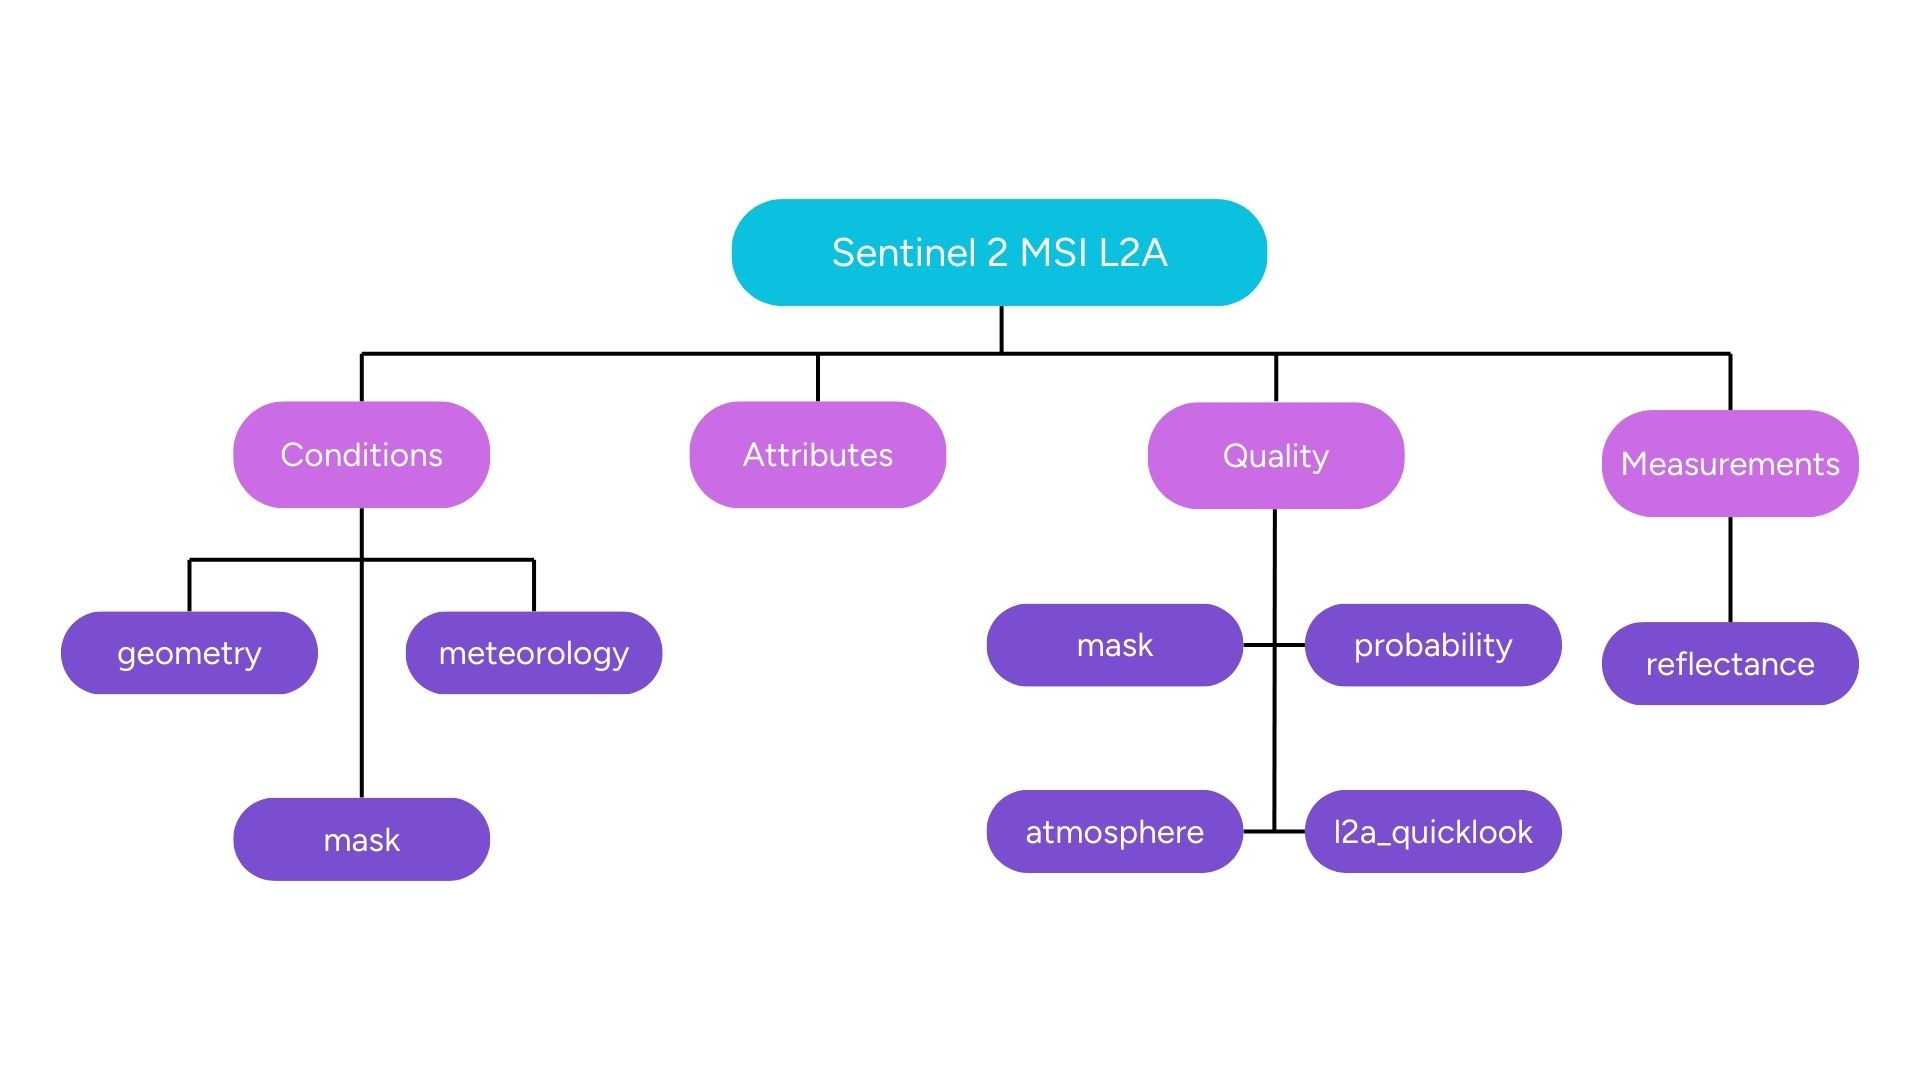
\includegraphics[keepaspectratio]{img/s2l2a.jpg}}
\end{center}

The table below provides a more detailed outline what content is
available in the different groups.

\begin{longtable}[]{@{}
  >{\raggedright\arraybackslash}p{(\linewidth - 4\tabcolsep) * \real{0.3333}}
  >{\raggedright\arraybackslash}p{(\linewidth - 4\tabcolsep) * \real{0.1905}}
  >{\raggedright\arraybackslash}p{(\linewidth - 4\tabcolsep) * \real{0.4762}}@{}}
\toprule\noalign{}
\begin{minipage}[b]{\linewidth}\raggedright
Group
\end{minipage} & \begin{minipage}[b]{\linewidth}\raggedright
\end{minipage} & \begin{minipage}[b]{\linewidth}\raggedright
Content
\end{minipage} \\
\midrule\noalign{}
\endhead
\bottomrule\noalign{}
\endlastfoot
\textbf{Attributes} & & Processing history metadata Chunking
configuration Global metadata (acquisition time, sensing time, etc.)
Product-specific metadata≈ \\
\textbf{Measurements} & \textbf{10m resolution (r10)} & B02 (Blue,
490nm) B03 (Green, 560nm) B04 (Red, 665nm) B08 (NIR, 842nm) \\
& \textbf{20m resolution (r20)} & B05 (Red Edge 1, 705nm) B06 (Red Edge
2, 740nm) B07 (Red Edge 3, 783nm) B8A (Narrow NIR, 865nm) B11 (SWIR 1,
1610nm) B12 (SWIR 2, 2190nm) \\
& \textbf{60m resolution (r60)} & B01 (Coastal aerosol, 443nm)
\textless br?B09 (Water vapour, 945nm) \\
\textbf{Conditions} & & Sun angles (zenith, azimuth) Viewing angles Mean
solar irradiance Atmospheric parameters such as (i) Aerosol Optical
Thickness (AOT), (ii) Water Vapor (WV) and (iii) Cloud and snow
probability \\
\textbf{Quality} & & Scene Classification Layer (SCL) Quality flags for
each band Detector footprint Defective pixels masks \\
\end{longtable}

\begin{tcolorbox}[enhanced jigsaw, coltitle=black, colback=white, leftrule=.75mm, colbacktitle=quarto-callout-note-color!10!white, titlerule=0mm, title=\textcolor{quarto-callout-note-color}{\faInfo}\hspace{0.5em}{Note}, rightrule=.15mm, bottomrule=.15mm, bottomtitle=1mm, toptitle=1mm, arc=.35mm, toprule=.15mm, left=2mm, opacityback=0, colframe=quarto-callout-note-color-frame, opacitybacktitle=0.6, breakable]

Zarr Deep Dive: Dive deeper into the benefits of Zarr in a blogpost by
Lindsey Nield from the Earthmover team:
\href{https://earthmover.io/blog/what-is-zarr}{Fundamentals: What is
Zarr? A Cloud-Native Format for Tensor Data}.

\end{tcolorbox}

\section{Conclusion}\label{conclusion-3}

The EOPF Zarr structure allows for efficient access to individual bands
or specific spatial regions without loading the entire dataset, making
it ideal for large-scale geospatial analysis. It further ensures all
relevant metadata is co-located with the data, enhancing data
discoverability and usability.

\section{What's next?}\label{whats-next-3}

Now that you have a theoretical grasp of the \textbf{Zarr} format, the
next section \href{./22_zarr_struct_S2L2A.ipynb}{Discover EOPF Zarr -
Sentinel-2 L2A} will provide a first hands-on experience opening an EOPF
Zarr product. We will transition to our first \textbf{Jupyter Notebook}
where you will directly interact with a Zarr store.

\chapter{Discover EOPF Zarr - Sentinel-2
L2A}\label{discover-eopf-zarr---sentinel-2-l2a}

\subsection{Introduction}\label{introduction-4}

This tutorial introduces you to the structure of a an EOPF Zarr product
sample for \textbf{Sentinel-2 L2A} data. We will demonstrate how to
access and open a Zarr product sample with \texttt{xarray}, how to
visualise the \texttt{zarr} encoding structure, explore embedded
information, and retrieve relevant metadata for further processing.

\subsection{What we will learn}\label{what-we-will-learn-3}

\begin{itemize}
\tightlist
\item
  ⚙️ How to open a \texttt{.zarr} file using \texttt{xarray}?
\item
  🛰️ The general structure of a Sentinel-2 L-2A item
\item
  🔎 How to access metadata that describes the \texttt{.zarr} encoding?
\end{itemize}

\subsection{Prerequisites}\label{prerequisites}

This tutorial uses a re-processed sample dataset from the
\href{https://stac.browser.user.eopf.eodc.eu/}{EOPF Sentinel Zarr
Samples Service STAC API} that is available for direct access
\href{https://objects.eodc.eu/e05ab01a9d56408d82ac32d69a5aae2a:202506-s02msil2a/10/products/cpm_v256/S2C_MSIL2A_20250610T103641_N0511_R008_T32UMD_20250610T132001.zarr}{here}.

The selected \texttt{zarr} product is a Sentinel-2 L2A tile from the
10th of June 2025: * File name:
\texttt{S2C\_MSIL2A\_20250610T103641\_N0511\_R008\_T32UMD\_20250610T132001.zarr.}).

\subsubsection{Import libraries}\label{import-libraries}

\begin{Shaded}
\begin{Highlighting}[]
\ImportTok{import}\NormalTok{ os}
\ImportTok{import}\NormalTok{ xarray }\ImportTok{as}\NormalTok{ xr}
\end{Highlighting}
\end{Shaded}

\subsubsection{Helper functions}\label{helper-functions}

\paragraph{\texorpdfstring{\texttt{print\_gen\_structure}}{print\_gen\_structure}}\label{print_gen_structure}

This function helps us to retrieve an visualise the names for each of
the stored groups inside a \texttt{zarr}. As an output, it will print a
general overview of elements inside the \texttt{zarr}.

\begin{Shaded}
\begin{Highlighting}[]
\KeywordTok{def}\NormalTok{ print\_gen\_structure(node, indent}\OperatorTok{=}\StringTok{""}\NormalTok{):}
    \BuiltInTok{print}\NormalTok{(}\SpecialStringTok{f"}\SpecialCharTok{\{}\NormalTok{indent}\SpecialCharTok{\}\{}\NormalTok{node}\SpecialCharTok{.}\NormalTok{name}\SpecialCharTok{\}}\SpecialStringTok{"}\NormalTok{)     }\CommentTok{\#allows us access each node}
    \ControlFlowTok{for}\NormalTok{ child\_name, child\_node }\KeywordTok{in}\NormalTok{ node.children.items(): }\CommentTok{\#loops inside the selected nodes to extract naming}
\NormalTok{        print\_gen\_structure(child\_node, indent }\OperatorTok{+} \StringTok{"  "}\NormalTok{) }\CommentTok{\# prints the name of the selected nodes}
\end{Highlighting}
\end{Shaded}

\section{Open a Zarr Store}\label{open-a-zarr-store}

In a first step, we use the function \texttt{open\_datatree()} from the
\texttt{xarray} library to open a Zarr store as a DataTree. Inside, we
ned to define the following key word arguments:

\begin{itemize}
\tightlist
\item
  \texttt{filename\_or\_obj}: path leading to a \texttt{zarr} store
\item
  \texttt{engine}:
  \texttt{\textquotesingle{}eopf-zarr\textquotesingle{}}, designed for
  the EOPF \texttt{zarr} by ESA.
\item
  \texttt{op\_mode}: extension by the \texttt{xarray-eopf} development
  for allowing an analysis or native mode. For more information visit
  the
  \href{https://eopf-sample-service.github.io/xarray-eopf/}{xarray-eopf}
  documentation.
\item
  \texttt{chunks}: loads the data with dask using the engine's preferred
  chunk size, generally identical to the format's chunk size
\end{itemize}

The final print of the \texttt{DataTree} object is commented out, as the
display can be quite extensive, showing the entire content within the
Zarr. An alternative is to apply a helper function that only displays
the higher level structure as shown in the next code cell.

\begin{Shaded}
\begin{Highlighting}[]
\NormalTok{url }\OperatorTok{=} \StringTok{\textquotesingle{}https://objects.eodc.eu/e05ab01a9d56408d82ac32d69a5aae2a:202506{-}s02msil2a/10/products/cpm\_v256/S2C\_MSIL2A\_20250610T103641\_N0511\_R008\_T32UMD\_20250610T132001.zarr\textquotesingle{}}
\NormalTok{s2l2a\_zarr\_sample}\OperatorTok{=}\NormalTok{ xr.open\_datatree(url,}
\NormalTok{    engine}\OperatorTok{=}\StringTok{"eopf{-}zarr"}\NormalTok{, }\CommentTok{\# storage format}
\NormalTok{    op\_mode}\OperatorTok{=}\StringTok{"native"}\NormalTok{, }\CommentTok{\# no analysis mode}
\NormalTok{    chunks}\OperatorTok{=}\NormalTok{\{\}, }\CommentTok{\# allows to open the default chunking}
\NormalTok{)}
\end{Highlighting}
\end{Shaded}

If we apply the helper function \texttt{print\_gen\_structure} on the
root of the DataTree object, we will get a listing of the tree-like
structure of the object. We can see all Zarr groups, such as
\texttt{measurements}, \texttt{quality} and \texttt{conditions}, their
sub-groups and content.

\begin{Shaded}
\begin{Highlighting}[]
\BuiltInTok{print}\NormalTok{(}\StringTok{"Zarr Sentinel 2 L2A Structure"}\NormalTok{)}
\NormalTok{print\_gen\_structure(s2l2a\_zarr\_sample.root) }
\BuiltInTok{print}\NormalTok{(}\StringTok{"{-}"} \OperatorTok{*} \DecValTok{30}\NormalTok{)}
\end{Highlighting}
\end{Shaded}

\begin{verbatim}
Zarr Sentinel 2 L2A Structure
None
  conditions
    geometry
    mask
      detector_footprint
        r10m
        r20m
        r60m
      l1c_classification
        r60m
      l2a_classification
        r20m
        r60m
    meteorology
      cams
      ecmwf
  measurements
    reflectance
      r10m
      r20m
      r60m
  quality
    atmosphere
      r10m
      r20m
      r60m
    l2a_quicklook
      r10m
      r20m
      r60m
    mask
      r10m
      r20m
      r60m
    probability
      r20m
------------------------------
\end{verbatim}

\section{Extract information from Zarr
groups}\label{extract-information-from-zarr-groups}

In a next step, we can explore the content of individual Zarr groups. By
specifying the name of the group and subgroup and adding it into square
brackets, we can extract the content of the relevant group. Let us for
example extract the content of the subgroup \texttt{reflectance} under
\texttt{measurements}.

As a result, it is visible that there are three subgroups of the parent
node \texttt{measurements/reflectance}: \texttt{r10}, \texttt{r20} and
\texttt{r60}, which are the DataArrays with the three different
resolutions of the Sentinel-2 L2A data.

The \texttt{xarray.DataTree} structure allows the exploration of
additional group-related metadata and information. For example, we can
find the \texttt{chunksize} of each array and the coordinates.

\begin{Shaded}
\begin{Highlighting}[]
\CommentTok{\# Retrieving the reflectance groups:}
\CommentTok{\# s2l2a\_zarr\_sample["measurements/reflectance"] \# Run it yourself for an inteactive overview}
\end{Highlighting}
\end{Shaded}

\section{Extract Zarr metadata on different
levels}\label{extract-zarr-metadata-on-different-levels}

Through \texttt{s2l2a\_zarr\_sample.attrs{[}{]}} we are able to
visualise both the \texttt{stac\_discovery} and \texttt{other\_metadata}
included in the \texttt{zarr} store. For the properties inside
\texttt{stac\_discovery} for example we can get the parameters included:

\begin{Shaded}
\begin{Highlighting}[]
\CommentTok{\# STAC metadata style:}
\BuiltInTok{print}\NormalTok{(}\BuiltInTok{list}\NormalTok{(s2l2a\_zarr\_sample.attrs[}\StringTok{"stac\_discovery"}\NormalTok{].keys()))}
\end{Highlighting}
\end{Shaded}

\begin{verbatim}
['assets', 'bbox', 'geometry', 'id', 'links', 'properties', 'stac_extensions', 'stac_version', 'type']
\end{verbatim}

We are also, able to retrieve specific information by diving deep into
the \texttt{stac\_discovery} metadata, such as:

\begin{Shaded}
\begin{Highlighting}[]
\BuiltInTok{print}\NormalTok{(}\StringTok{\textquotesingle{}Date of Item Creation: \textquotesingle{}}\NormalTok{, s2l2a\_zarr\_sample.attrs[}\StringTok{\textquotesingle{}stac\_discovery\textquotesingle{}}\NormalTok{][}\StringTok{\textquotesingle{}properties\textquotesingle{}}\NormalTok{][}\StringTok{\textquotesingle{}created\textquotesingle{}}\NormalTok{])}
\BuiltInTok{print}\NormalTok{(}\StringTok{\textquotesingle{}Item Bounding Box    : \textquotesingle{}}\NormalTok{, s2l2a\_zarr\_sample.attrs[}\StringTok{\textquotesingle{}stac\_discovery\textquotesingle{}}\NormalTok{][}\StringTok{\textquotesingle{}bbox\textquotesingle{}}\NormalTok{])}
\BuiltInTok{print}\NormalTok{(}\StringTok{\textquotesingle{}Item ESPG            : \textquotesingle{}}\NormalTok{, s2l2a\_zarr\_sample.attrs[}\StringTok{\textquotesingle{}stac\_discovery\textquotesingle{}}\NormalTok{][}\StringTok{\textquotesingle{}properties\textquotesingle{}}\NormalTok{][}\StringTok{\textquotesingle{}proj:epsg\textquotesingle{}}\NormalTok{])}
\BuiltInTok{print}\NormalTok{(}\StringTok{\textquotesingle{}Sentinel Platform    : \textquotesingle{}}\NormalTok{, s2l2a\_zarr\_sample.attrs[}\StringTok{\textquotesingle{}stac\_discovery\textquotesingle{}}\NormalTok{][}\StringTok{\textquotesingle{}properties\textquotesingle{}}\NormalTok{][}\StringTok{\textquotesingle{}platform\textquotesingle{}}\NormalTok{])}
\BuiltInTok{print}\NormalTok{(}\StringTok{\textquotesingle{}Item Processing Level: \textquotesingle{}}\NormalTok{, s2l2a\_zarr\_sample.attrs[}\StringTok{\textquotesingle{}stac\_discovery\textquotesingle{}}\NormalTok{][}\StringTok{\textquotesingle{}properties\textquotesingle{}}\NormalTok{][}\StringTok{\textquotesingle{}processing:level\textquotesingle{}}\NormalTok{])}
\end{Highlighting}
\end{Shaded}

\begin{verbatim}
Date of Item Creation:  2025-06-10T13:20:01+00:00
Item Bounding Box    :  [9.146276872400831, 52.25344953517325, 7.500940412097549, 53.24953673463324]
Item ESPG            :  32632
Sentinel Platform    :  sentinel-2c
Item Processing Level:  L2A
\end{verbatim}

And from \texttt{other\_metadata}, we are able to retrieve the
information specific to the instrument variables.

\begin{Shaded}
\begin{Highlighting}[]
\CommentTok{\# Complementing metadata:}
\BuiltInTok{print}\NormalTok{(}\BuiltInTok{list}\NormalTok{(s2l2a\_zarr\_sample.attrs[}\StringTok{"other\_metadata"}\NormalTok{].keys()))}
\end{Highlighting}
\end{Shaded}

\begin{verbatim}
['AOT_retrieval_model', 'L0_ancillary_data_quality', 'L0_ephemeris_data_quality', 'NUC_table_ID', 'SWIR_rearrangement_flag', 'UTM_zone_identification', 'absolute_location_assessment_from_AOCS', 'band_description', 'declared_accuracy_of_AOT_model', 'declared_accuracy_of_radiative_transfer_model', 'declared_accuracy_of_water_vapour_model', 'electronic_crosstalk_correction_flag', 'eopf_category', 'geometric_refinement', 'history', 'horizontal_CRS_code', 'horizontal_CRS_name', 'mean_sensing_time', 'mean_sun_azimuth_angle_in_deg_for_all_bands_all_detectors', 'mean_sun_zenith_angle_in_deg_for_all_bands_all_detectors', 'mean_value_of_aerosol_optical_thickness', 'mean_value_of_total_water_vapour_content', 'meteo', 'multispectral_registration_assessment', 'onboard_compression_flag', 'onboard_equalization_flag', 'optical_crosstalk_correction_flag', 'ozone_source', 'ozone_value', 'percentage_of_degraded_MSI_data', 'planimetric_stability_assessment_from_AOCS', 'product_quality_status', 'reflectance_correction_factor_from_the_Sun-Earth_distance_variation_computed_using_the_acquisition_date', 'spectral_band_of_reference']
\end{verbatim}

\section{💪 Now it is your turn}\label{now-it-is-your-turn}

As we are able to retrieve several items from the
\href{https://stac.browser.user.eopf.eodc.eu/}{EOPF Sentinel Zarr
Samples Service STAC API}, let us try the following: \#\#\# Task Go to
the
\href{https://stac.browser.user.eopf.eodc.eu/collections/sentinel-2-l2a}{Sentinel-2
Level-2A collection} and: - Choose an item of interest. - Replicate the
workflow and explore the item's metadata. When was it retrieved? - What
are the dimensions? - What is the detailed location of the item?

\section{Conclusion}\label{conclusion-4}

This tutorial provides an initial understanding of the \texttt{zarr}
structure for a Sentinel-2 L2A product sample. By using the
\texttt{xarray} library, we can effectively navigate and inspect the
different components within the \texttt{zarr} format, including its
metadata and array organisation.

\section{What's next?}\label{whats-next-4}

Now that you've been introduced to the \texttt{zarr} format, learned its
core concepts, and understood the basics of how to explore it, you are
prepared for the next step. In the following
\href{./31_stac_intro.qmd}{chapter} we will introduce you to
\textbf{STAC} and the \textbf{EOPF Zarr STAC Catalog}. As we go along,
we are more and more transition from theory to practice, providing you
with hands-on tutorials working with EOPF Zarr products.

\part{\textbf{EOPF and STAC}}

\chapter{Introduction to STAC}\label{introduction-to-stac}

\subsection{Introduction}\label{introduction-5}

Welcome to the chapter on EOPF and STAC. In the following section, we
will introduce you to the the \textbf{S}patio-\textbf{T}emporal
\textbf{A}sset \textbf{C}atalog (STAC). We will explain its fundamental
principles and, most importantly, we will explore its structure and core
components. Understanding the fundamentals of STAC is key in order to be
able effectively discover and access data from STAC catalogs.

\subsection{What we will learn}\label{what-we-will-learn-4}

\begin{itemize}
\tightlist
\item
  🔍 What STAC is and why it is important?
\item
  🌳 Navigate through the STAC ecosystem, and
\item
  🪜📊 Understand the main components of STAC
\end{itemize}

\section{About STAC}\label{about-stac}

The \textbf{S}patio-\textbf{T}emporal \textbf{A}sset \textbf{C}atalog
(STAC) is a standardised way to catalog and describe geospatial (raster)
data. STAC makes it easier to discover, access, and work with geospatial
data, in particular satellite data, as it provides a \textbf{common
language for describing spatial and temporal characteristics} of the
data. This common language improves interoperability between different
data providers and software tools.

The main goal of \href{https://stacspec.org/en/}{STAC} is to allow data
providers share their data easily, making it universal for users to
understand the where, when, how, and what of the collected data.

STAC uses \textbf{JSON} (JavaScript Object Notion) to structure the
metadata of geo-referenced datasets. JSON makes it machine-readable.
Through it is design, STAC is simple and extensible in its design as it
is based on a network of JSON files.

STAC has evolved into a well-recognised community standard. The key
benefit supporting its wide adoption is that one can use the same code
and API to access data from different data repositories.

\section{The STAC ecosystem}\label{the-stac-ecosystem}

STAC has evolved in a vast ecosystem offering various resources and
tools for accessing, managing, and building STAC catalogs. Below is a
non-exclusive list of tools and plug-ins that will help to explore the
STAC ecosystem:

\begin{longtable}[]{@{}
  >{\raggedright\arraybackslash}p{(\linewidth - 6\tabcolsep) * \real{0.0551}}
  >{\raggedright\arraybackslash}p{(\linewidth - 6\tabcolsep) * \real{0.0636}}
  >{\raggedright\arraybackslash}p{(\linewidth - 6\tabcolsep) * \real{0.8390}}
  >{\raggedright\arraybackslash}p{(\linewidth - 6\tabcolsep) * \real{0.0424}}@{}}
\toprule\noalign{}
\begin{minipage}[b]{\linewidth}\raggedright
Category
\end{minipage} & \begin{minipage}[b]{\linewidth}\raggedright
Tool/Plugin
\end{minipage} & \begin{minipage}[b]{\linewidth}\raggedright
Description
\end{minipage} & \begin{minipage}[b]{\linewidth}\raggedright
Language
\end{minipage} \\
\midrule\noalign{}
\endhead
\bottomrule\noalign{}
\endlastfoot
\textbf{STAC Tools} &
\href{https://github.com/radiantearth/stac-browser}{STAC Browser} & A
user-friendly web interface for visually exploring and interacting with
various STAC catalogs. & Web interface \\
& \href{https://github.com/stac-utils/stac-server}{STAC Server} & A
reference implementation for serving STAC catalogs and collections. &
Python \\
\textbf{STAC libraries and plug-ins} &
\href{https://github.com/stac-utils/stac-validator}{STAC Validator} & A
tool for programmatically validating STAC Catalogs, Collections, and
Items to ensure compliance with the STAC specification. & Python \\
& \href{https://github.com/stac-utils/pystac}{PySTAC} & A Python library
for reading, writing, and validating STAC objects, facilitating the
creation and manipulation of STAC data. & Python \\
& \href{https://pystac-client.readthedocs.io/en/stable/}{pystac-client}
& A Python library that provides a convenient and powerful interface for
searching and accessing STAC data from STAC API servers. & Python \\
& \href{https://github.com/brazil-data-cube/rstac}{rstac} & An R package
that provides functionalities for interacting with STAC APIs and working
with STAC objects within the R environment. & R \\
& \href{https://github.com/JuliaClimate/STAC.jl}{STAC.jl} & A Julia
package designed for working with STAC, enabling users to interact with
STAC catalogs and process geospatial data. & Julia \\
& \href{https://github.com/felixcremer/STACCube.jl}{STACCube.jl} & A
Julia package that facilitates the creation and management of
STAC-compliant data cubes from various geospatial datasets. & Julia \\
\end{longtable}

\section{STAC components}\label{stac-components}

Now, let us start exploring the structure of STAC. STAC consists of four
main components: (i) \texttt{Catalog}, (ii) \texttt{Collection}, (iii)
\texttt{Item} and (iv) \texttt{Asset}. See figure below for a principle
organisation of the STAC components.

\begin{figure}[H]

{\centering \pandocbounded{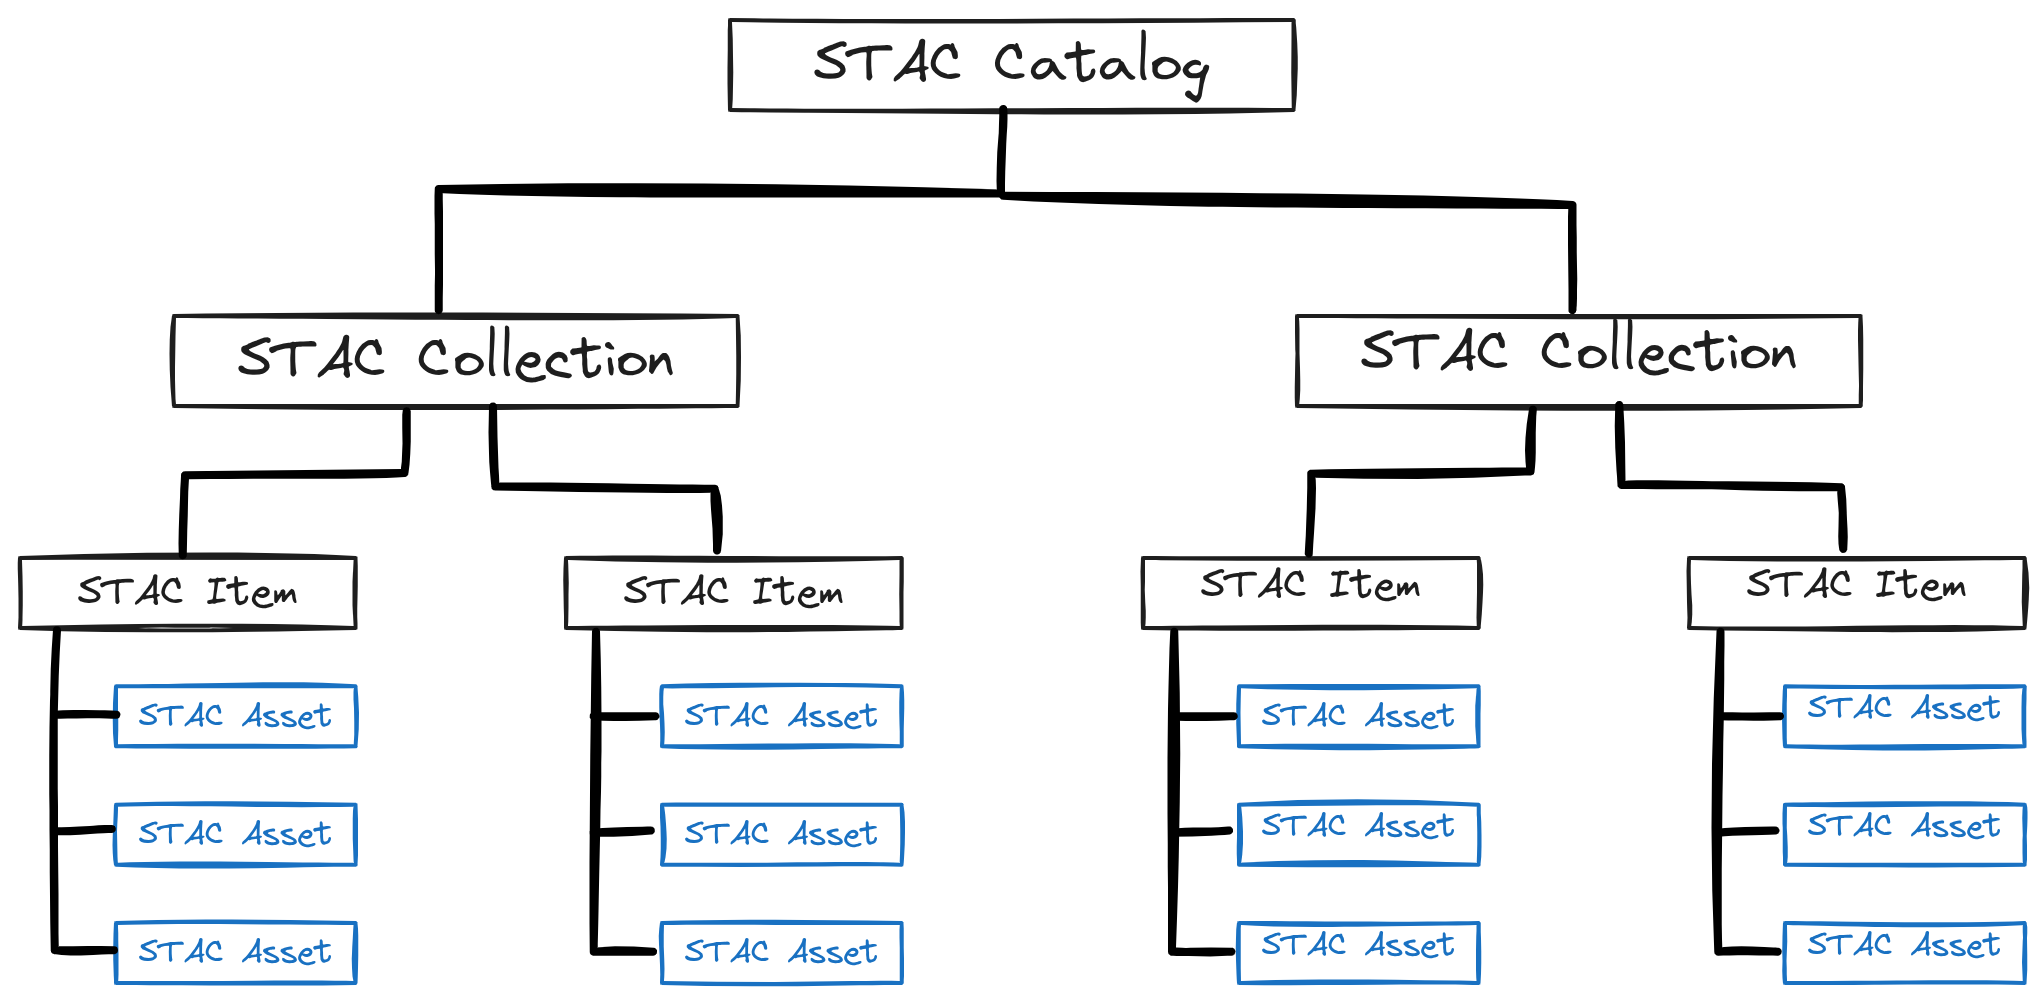
\includegraphics[keepaspectratio]{img/stac_example.png}}

}

\caption{STAC structure}

\end{figure}%

Let us now explore more in detail the individual components:

\subsection{Catalog}\label{catalog}

A \texttt{Catalog} serves as the initial entry point of a STAC. A
catalog is a very simple construct, it simply provides links to
\texttt{Collections} or \texttt{Items}. The closest analog is a folder
on your computer. A \texttt{Catalog} can be a \emph{folder} for
\texttt{Items}, but it can also be a \texttt{folder} for
\texttt{Collections} or other \texttt{Catalogs}. When searching for
specific data, you first establish a connection to a valid STAC catalog.

\subsection{Collection}\label{collection}

Collections are containers that support the grouping of \texttt{Items}.
The \texttt{Collection} entity shares most fields with the
\texttt{Catalog} entity but has a number of additional fields, such as
license, extent (spatial and temporal), providers, keywords and
summaries. Every \texttt{Item} in a \texttt{Collection} links back to
its \texttt{Collection}. \texttt{Collection} are often used to provide
additional structure in a STAC catalog.

\begin{tcolorbox}[enhanced jigsaw, coltitle=black, colback=white, leftrule=.75mm, colbacktitle=quarto-callout-note-color!10!white, titlerule=0mm, title=\textcolor{quarto-callout-note-color}{\faInfo}\hspace{0.5em}{Note}, rightrule=.15mm, bottomrule=.15mm, bottomtitle=1mm, toptitle=1mm, arc=.35mm, toprule=.15mm, left=2mm, opacityback=0, colframe=quarto-callout-note-color-frame, opacitybacktitle=0.6, breakable]

But when to use a \texttt{Collection} versus a \texttt{Catalog}? A
\texttt{Collection} generally consist of a set of assets that share the
same properties and share higher level metadata. For example data from
the same satellite sensor or constellation would typically be in on
\texttt{Collection}.

\texttt{Catalogs} in turn are used to plit overly large
\texttt{Collections} into groups and to group collections into a catalog
of Collections (e.g.~as entry point for navigation to several
Collections).

It is recommended to use \texttt{Collections} for what you want users to
find and \texttt{Catalogs} for structuring and grouping
\texttt{Collections}.

\end{tcolorbox}

\subsection{Item}\label{item}

An \texttt{Item} is the fundamental element of STAC and typically
represents a single scene at one place and time. It is a
\texttt{.GeoJSON} supplemented with additional metadata, which serves as
an index to \texttt{Assets}.

\begin{figure}[H]

{\centering \pandocbounded{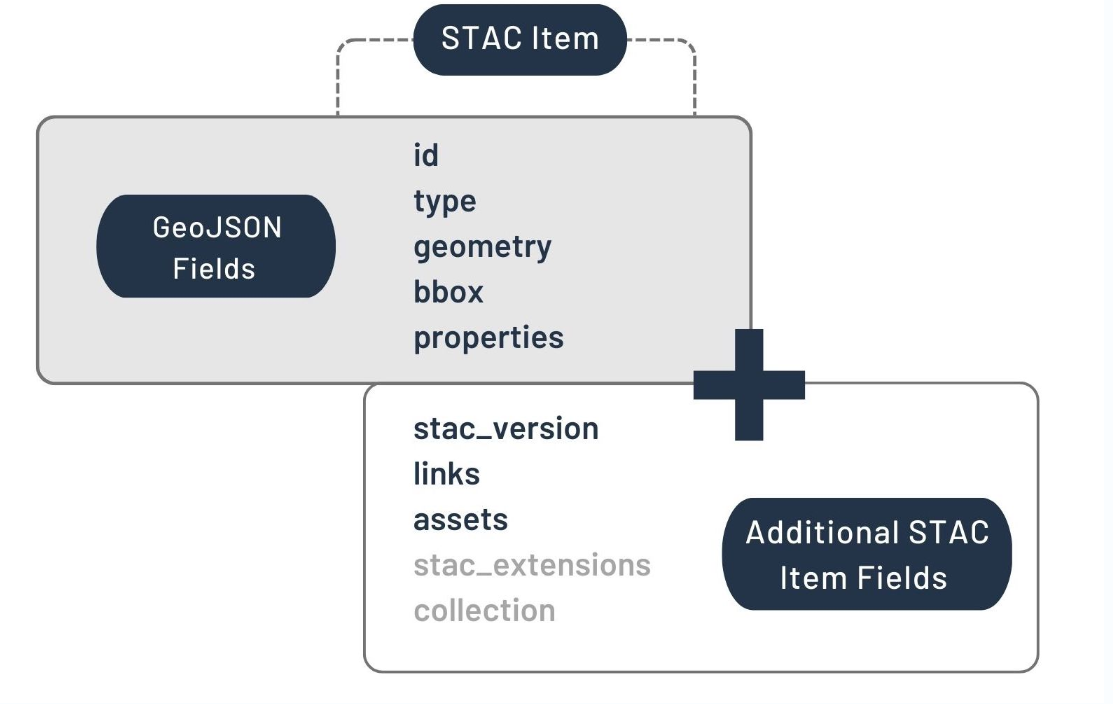
\includegraphics[keepaspectratio]{img/item_inf.png}}

}

\caption{Item entity}

\end{figure}%

\subsection{Asset}\label{asset}

An \texttt{Asset} is the smallest element inside a STAC and represent
the individual data file that is linked in a STAC \texttt{Item}.

\subsection{Analogy: Organising a drinks menu as a
STAC}\label{analogy-organising-a-drinks-menu-as-a-stac}

To better understand the relation of STAC components, let us imagine a
\textbf{Drinks} menu as a STAC. How would you structure \emph{Drinks} as
a STAC?

Let us start with the \emph{Drinks} a category themselves. The menu is
analog to a STAC \texttt{Catalog}, as it serves as the top-level entry
point, providing an overview of all beverages available.

Within this Drinks \textbf{catalog}, we can group the \emph{Drinks}
further in There are hot and cold beverages, caffeinated and
non-caffeinated drinks. These categories represent \textbf{Collections}
in STAC. For our analogy, let us say the menu is divided into two main
collections:

\begin{itemize}
\tightlist
\item
  \textbf{Caffeinated Drinks Collection}: This section groups all
  beverages that contain caffeine.
\item
  \textbf{Non-Caffeinated Drinks Collection}: This section groups all
  beverages that do not contain caffeine.
\end{itemize}

Each of these collections contains specific drinks, which are analog to
STAC \textbf{Items}. Drink \texttt{Items} could be e.g.~Juices or Milks.
Both represent again a group of specific juices and milks, which are
analog of \texttt{Assets} in STAC. For the Drink \texttt{Items} defined,
their \texttt{Assets} might include:

\begin{longtable}[]{@{}ll@{}}
\toprule\noalign{}
Item & Assets \\
\midrule\noalign{}
\endhead
\bottomrule\noalign{}
\endlastfoot
Milks & Oat Milk Regular Milk \\
Juices & Apple Juice Organge Juice \ldots{} \\
\end{longtable}

The STAC structure allows us to easily navigate a vast amount of data,
just as a well-organised menu helps a customer quickly find their
desired drink.

\begin{figure}[H]

{\centering \pandocbounded{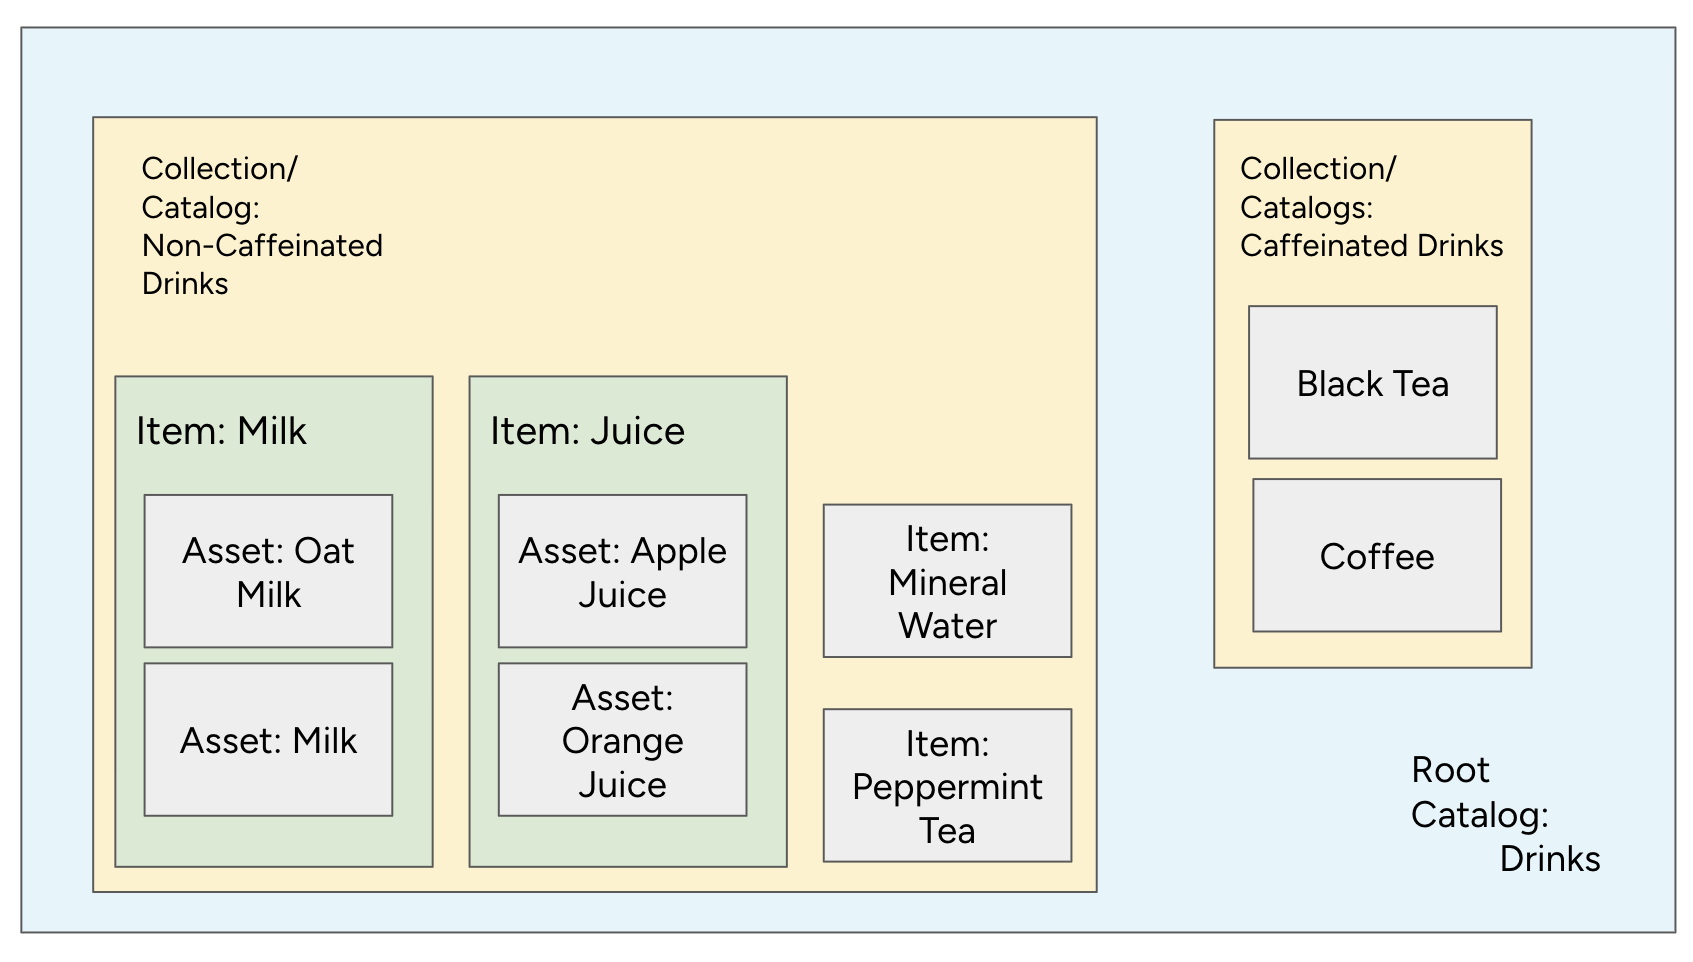
\includegraphics[keepaspectratio]{img/drinks_menu.png}}

}

\caption{Drinks Menu as a STAC analogy}

\end{figure}%

\section{Conclusion}\label{conclusion-5}

In this section you got an introduction to the \textbf{Spatio-Temporal
Asset Catalog} (STAC) and learned what STAC is and explored the main
components of a STAC. Understanding the distinction between
\texttt{Catalog}, \texttt{Collection}, \texttt{Items} and
\texttt{Assets} is important to effectively navigating through STAC
APIs.

\section{What's next?}\label{whats-next-5}

In the following \href{./32_eopf_stac_zarr_tutorial.qmd}{section}, we
will explore the web interface of the
\href{https://stac.browser.user.eopf.eodc.eu/?.language=en}{EOPF
Sentinel Zarr Samples Service STAC Catalog}.

\chapter{Explore the web interface of the EOPF Zarr STAC
Catalog}\label{explore-the-web-interface-of-the-eopf-zarr-stac-catalog}

\subsection{Introduction}\label{introduction-6}

This section introduces you to the
\href{https://stac.browser.user.eopf.eodc.eu/?.language=en}{EOPF
Sentinel Zarr Samples Service STAC Catalog}, which offers access to the
re-engineered Sentinel-1, Sentinel-2 and Sentinel-3 data products. We
will guide you through its web interface, inspect the various levels of
STAC components, and demonstrate how to access the underlying Sentinel
Zarr data.

\subsection{What we will learn}\label{what-we-will-learn-5}

\begin{itemize}
\tightlist
\item
  ⚙️ How does the STAC browser interface works
\item
  🔦 Explore the available Collections within the EOPF Sentinel Zarr
  Samples Service STAC Catalog
\item
  📡 How to obtain access to EOPF Sentinel Zarr products from the EOPF
  Sentinel Zarr Samples Service STAC Catalog
\end{itemize}

\section{Our Starting Point}\label{our-starting-point}

The first step is to access the main homepage of the
\href{https://stac.browser.user.eopf.eodc.eu/?.language=en}{EOPF
Sentinel Zarr Samples Service STAC Catalog}. The landing page offers you
a comprehensive overview of the available data collections. This serves
as our \textbf{initial entry} point into the catalog.

\begin{figure}[H]

{\centering \pandocbounded{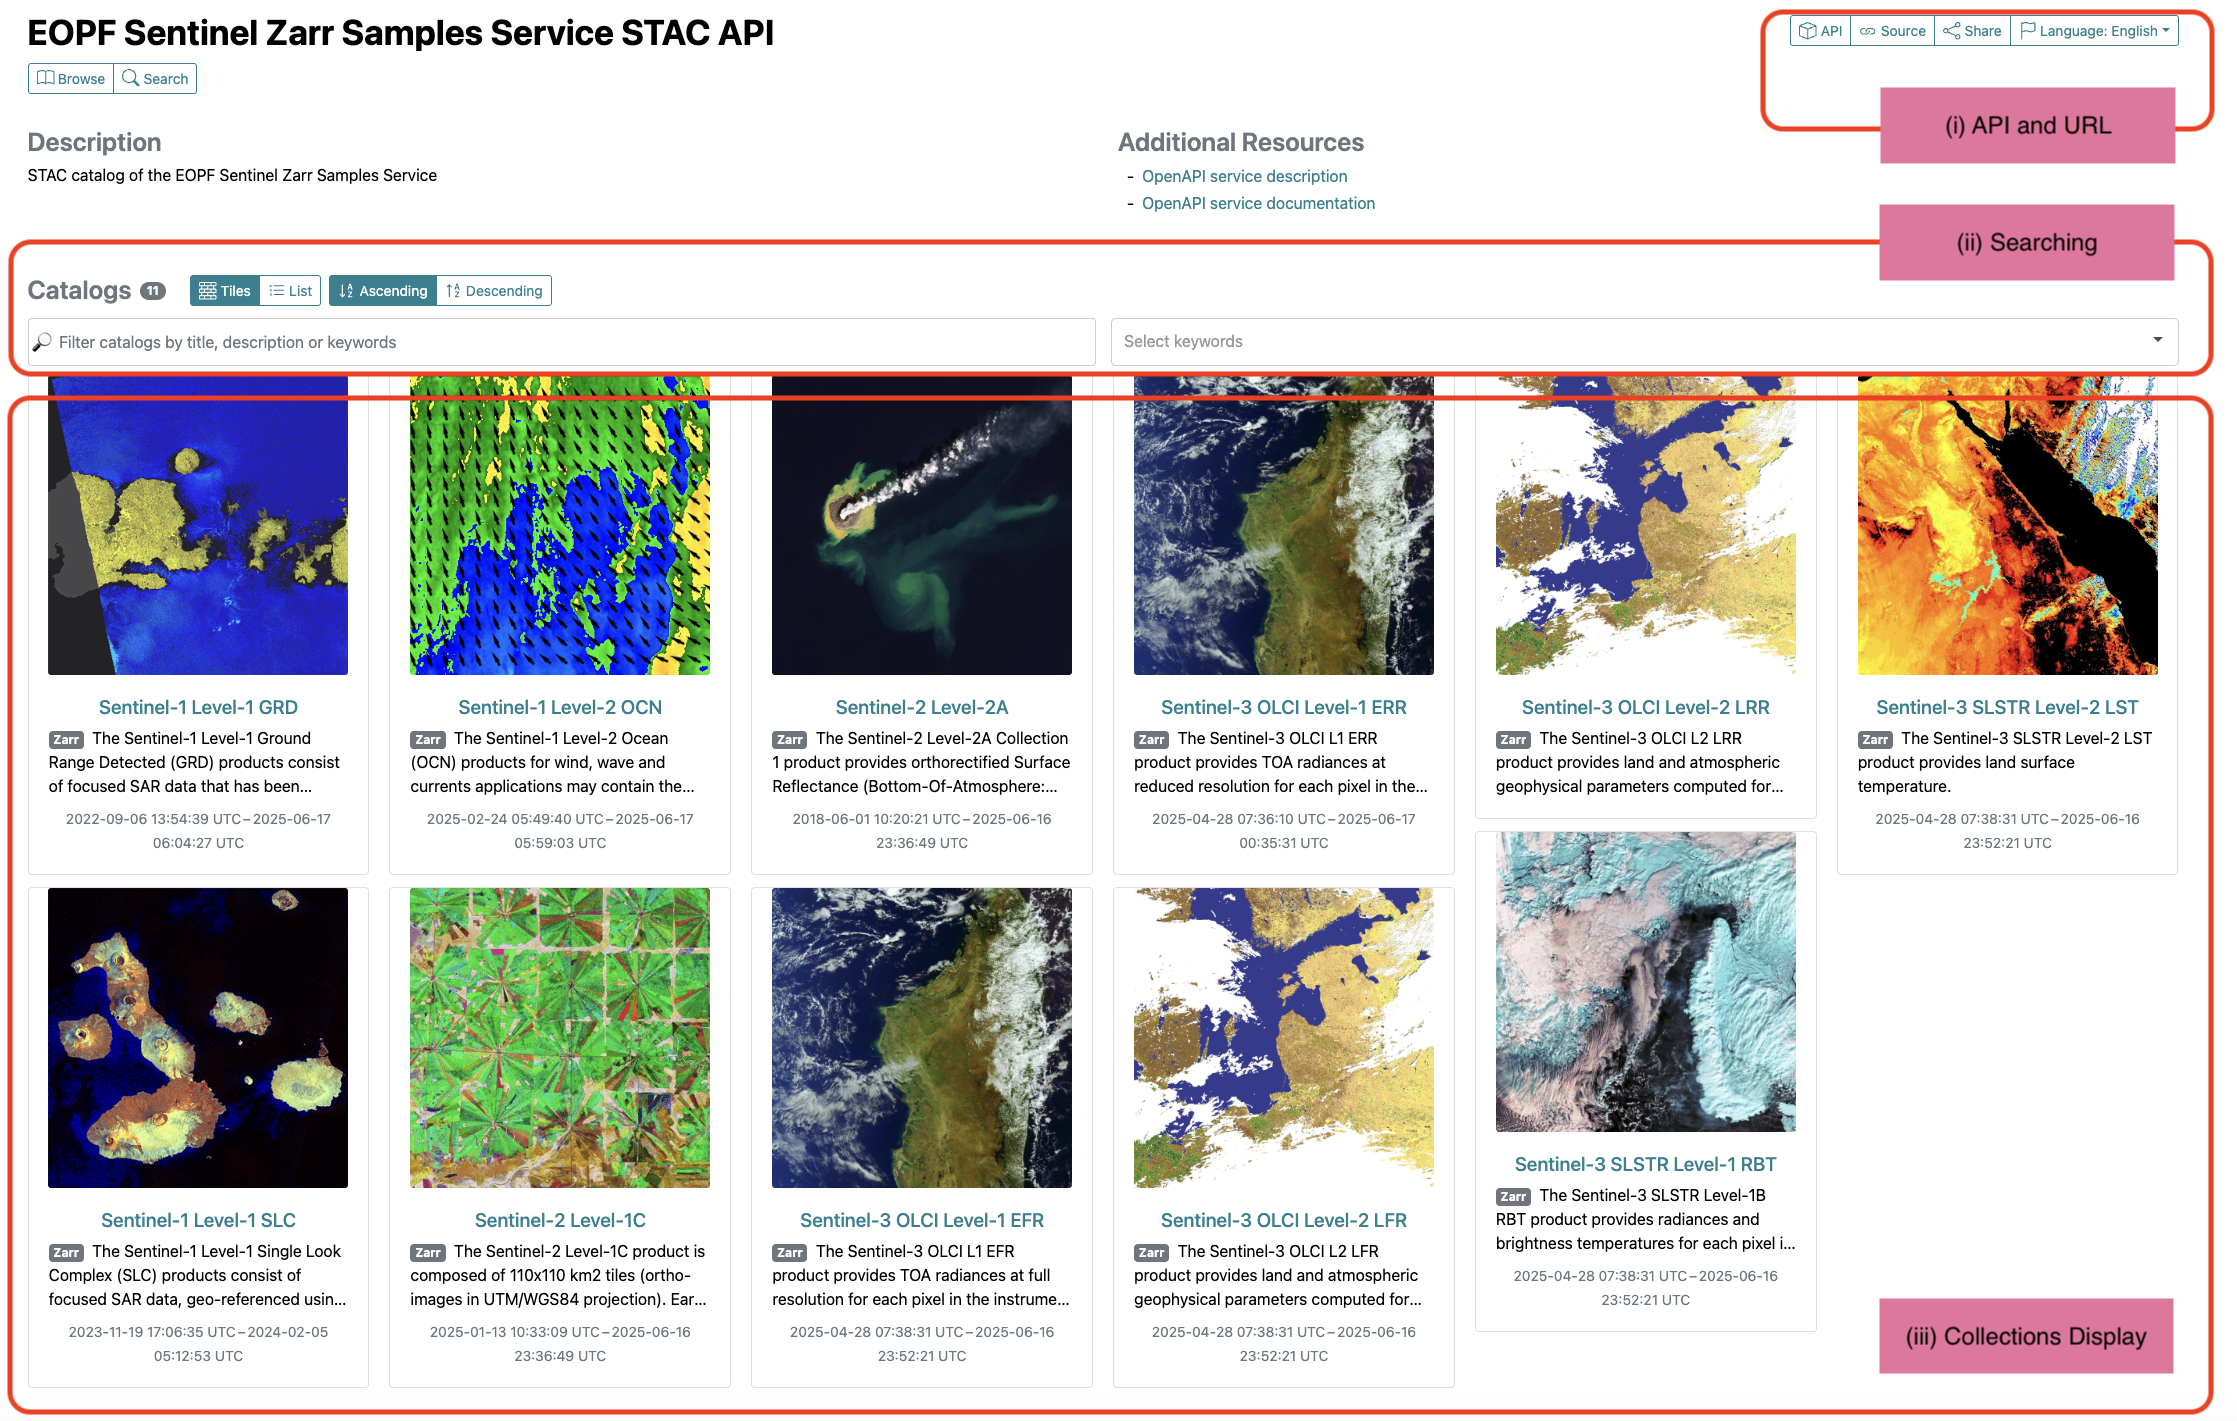
\includegraphics[keepaspectratio]{img/home_page.png}}

}

\caption{Home page}

\end{figure}%

Three main areas can be identified: (i) the \textbf{API and URL}
section, (ii) \textbf{Search bar} and (iii) \textbf{Collections
Display}.

As outlined in detail in the book section
\hyperref[overview-of-eopf-zarr-products]{The EOPF Available Datasets},
the catalog displays~the 11 distinct collections~available from the
Sentinel-1, Sentinel-2, and Sentinel-3 missions. The user interface
provides an intuitive way to browse through all of these collections. It
is possible to filter them by specific criteria or select them manually,
allowing precise control over the displayed data.

\section{Exploring Sentinel
Collections}\label{exploring-sentinel-collections}

Let us now select one of the 11 \texttt{Collection} available, e.g.~let
us select the
\href{https://stac.browser.user.eopf.eodc.eu/collections/sentinel-2-l2a}{Sentinel
2-Level-2A} collection. Once you selected the Collection, you will be
directed to the interface of a specific \texttt{Collection}.

\begin{figure}[H]

{\centering \pandocbounded{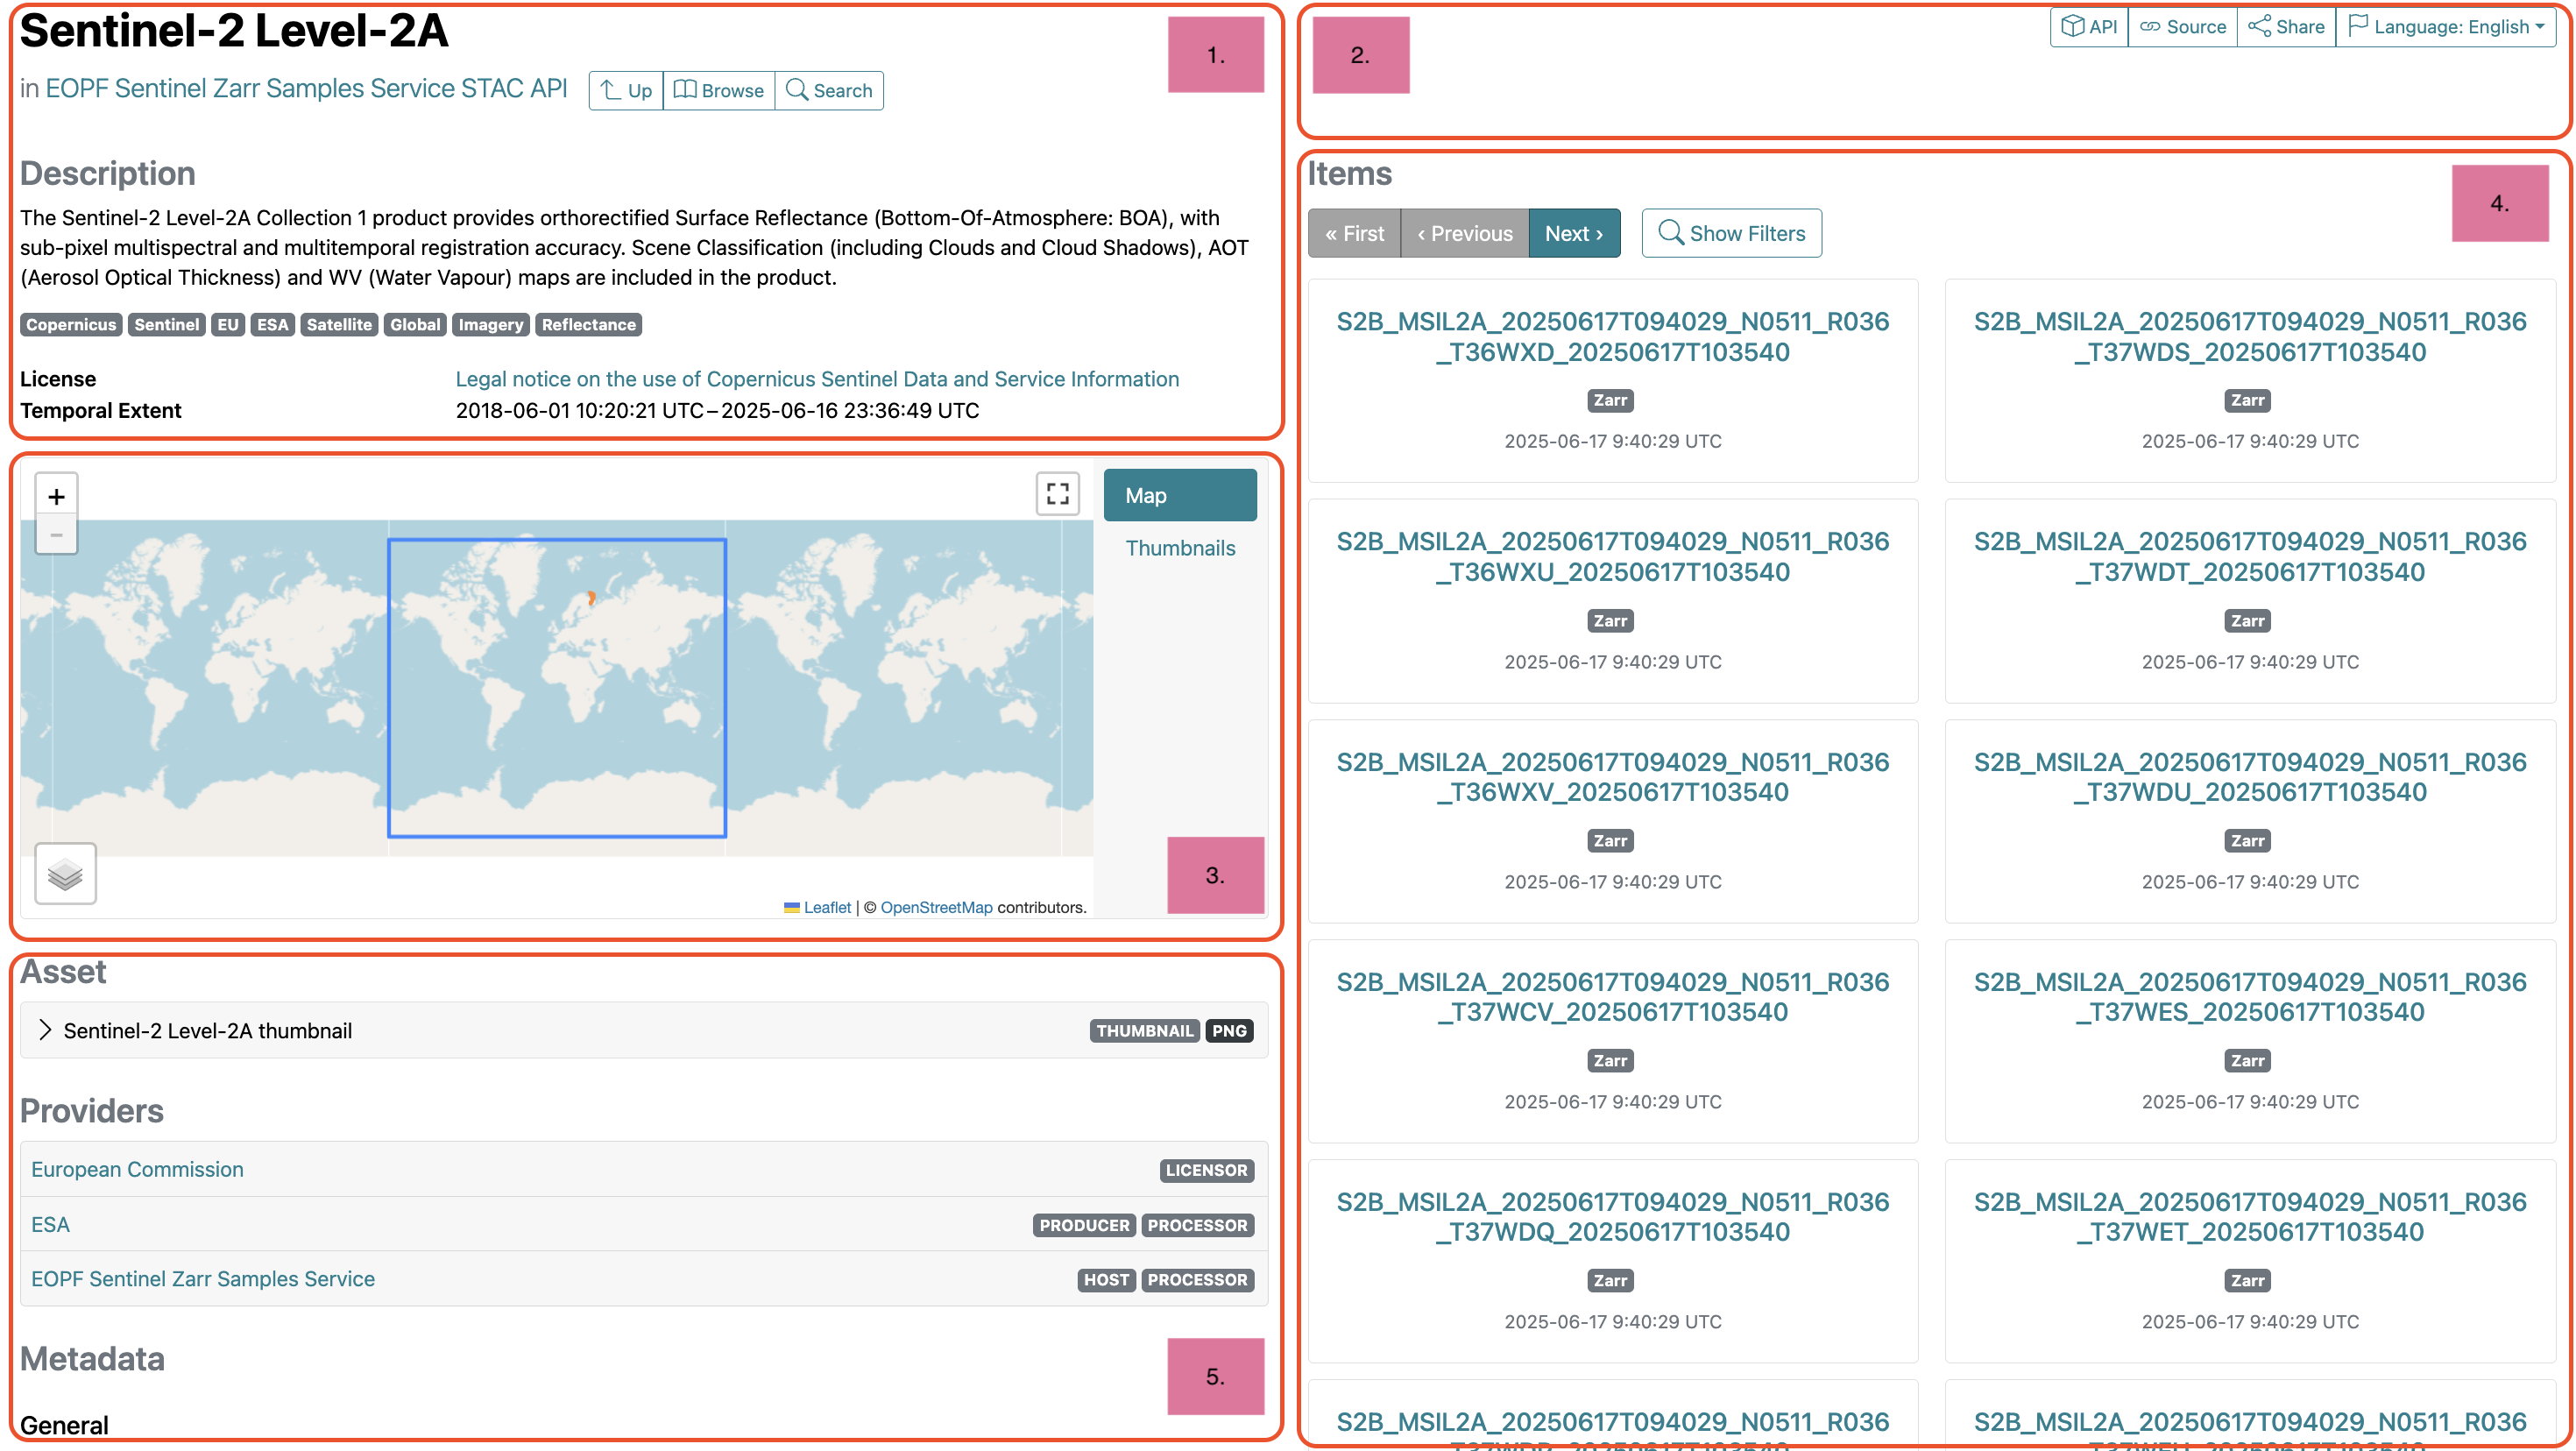
\includegraphics[keepaspectratio]{img/sentinel_2_collection.png}}

}

\caption{Web interface of the Sentinel-2 Level-2A Collection of the EOPF
Sentinel Zarr Samples Service STAC Catalog}

\end{figure}%

The interface can be divided into five principle sections:

\begin{enumerate}
\def\labelenumi{\arabic{enumi}.}
\tightlist
\item
  \textbf{Description}: The name and a brief introduction to the
  available collection. This includes crucial details such as the
  \textbf{temporal extent} (the period over which the data was acquired)
\item
  \textbf{API and URL}: for further application.
\item
  \textbf{Spatial Extent}: The geographical area of the displayed items
  is shown on the map.
\item
  \textbf{Available Items}: On the right-hand side of the page, a list
  of links for the items contained within the collection corresponds to
  the selected collection.
\item
  \textbf{Collection Metadata}: A general overview of the Collection's
  metadata, its providers, instruments, and the corresponding DOIs for
  research.
\item
  \textbf{Metadata}: Specific information about the bands and
  instruments such as backscatter or reflectance information.
\item
  \textbf{Assets in Items}: The Assets structure available for the Items
  available in the Collection.
\end{enumerate}

\subsection{Filtering Collections}\label{filtering-collections}

Any selected \texttt{Collection} (in this case Sentinel-2 Level-2A)
allows us to filter the items of our interest by \textbf{temporal} and
\textbf{spatial} extent. We can access this tab by clicking on
\textbf{Show Filters} on the right side under the \textbf{Items}
section.

\begin{figure}[H]

{\centering \pandocbounded{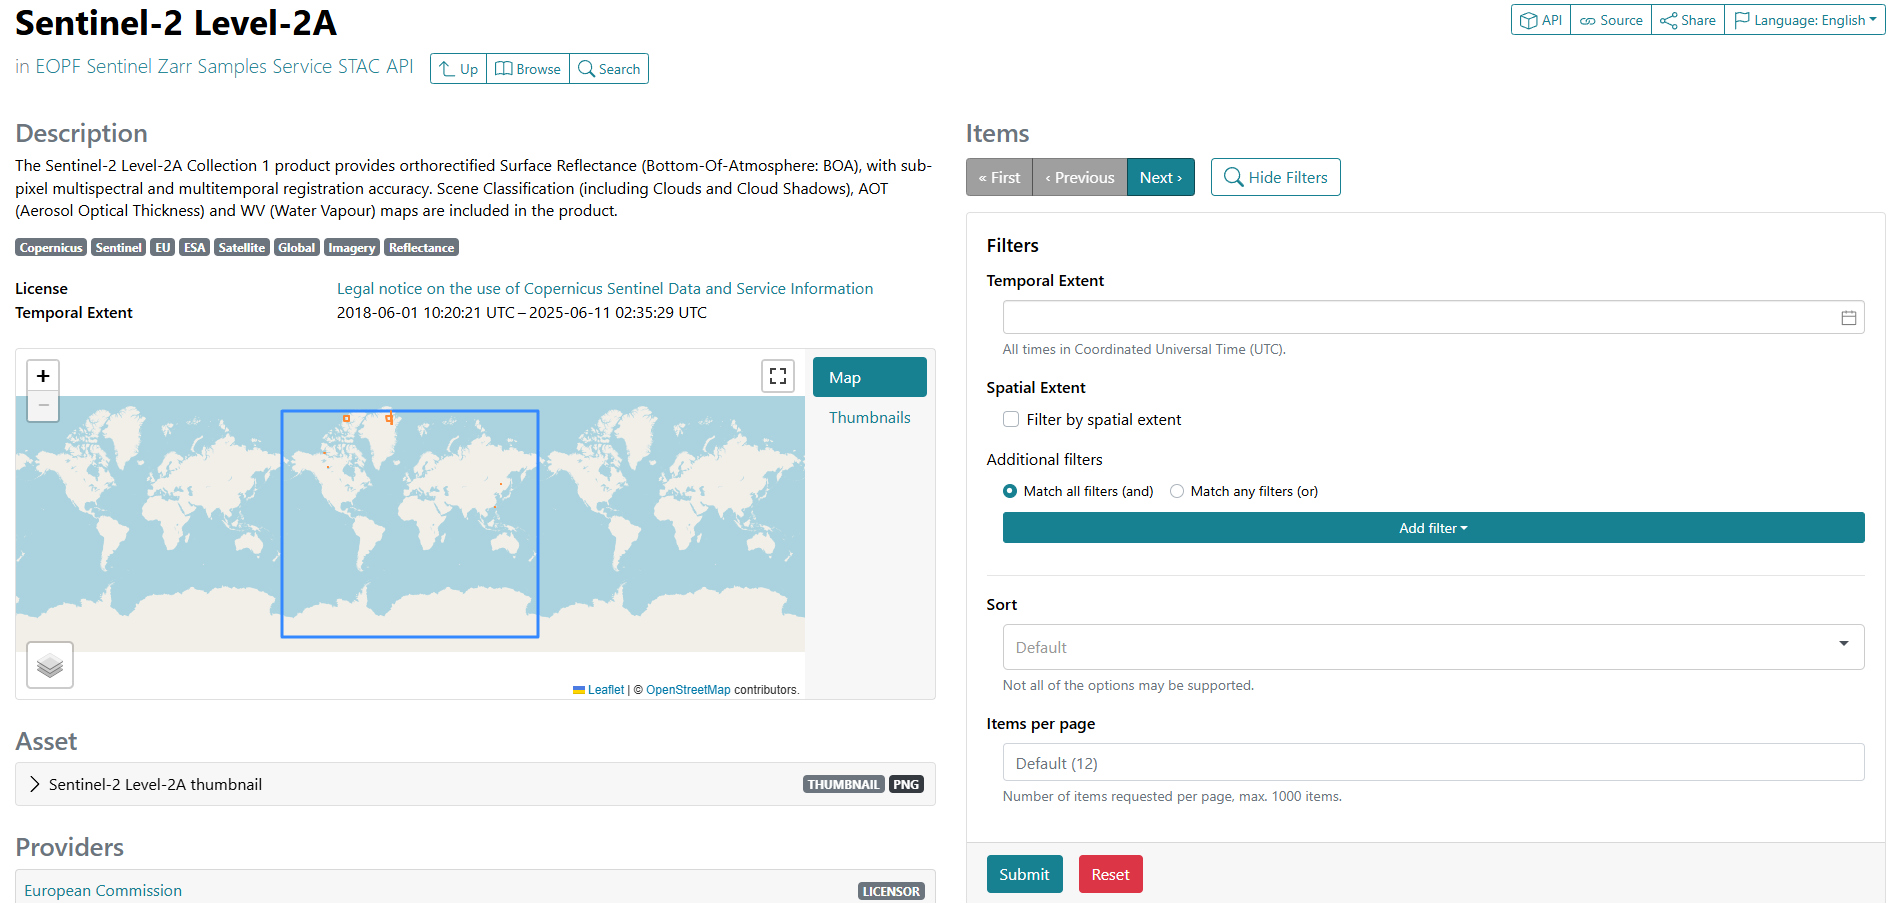
\includegraphics[keepaspectratio]{img/filter_1.png}}

}

\caption{Overview of interface that opens when clicking in \emph{Show
Filters}}

\end{figure}%

The interface the opens allows us to select on the calendar a specific
period we are interested in. This is particularly useful when we are
interested in a temporal analysis. Let us search over available items
captured between May 1st and May 5th 2024.

\begin{figure}[H]

{\centering \pandocbounded{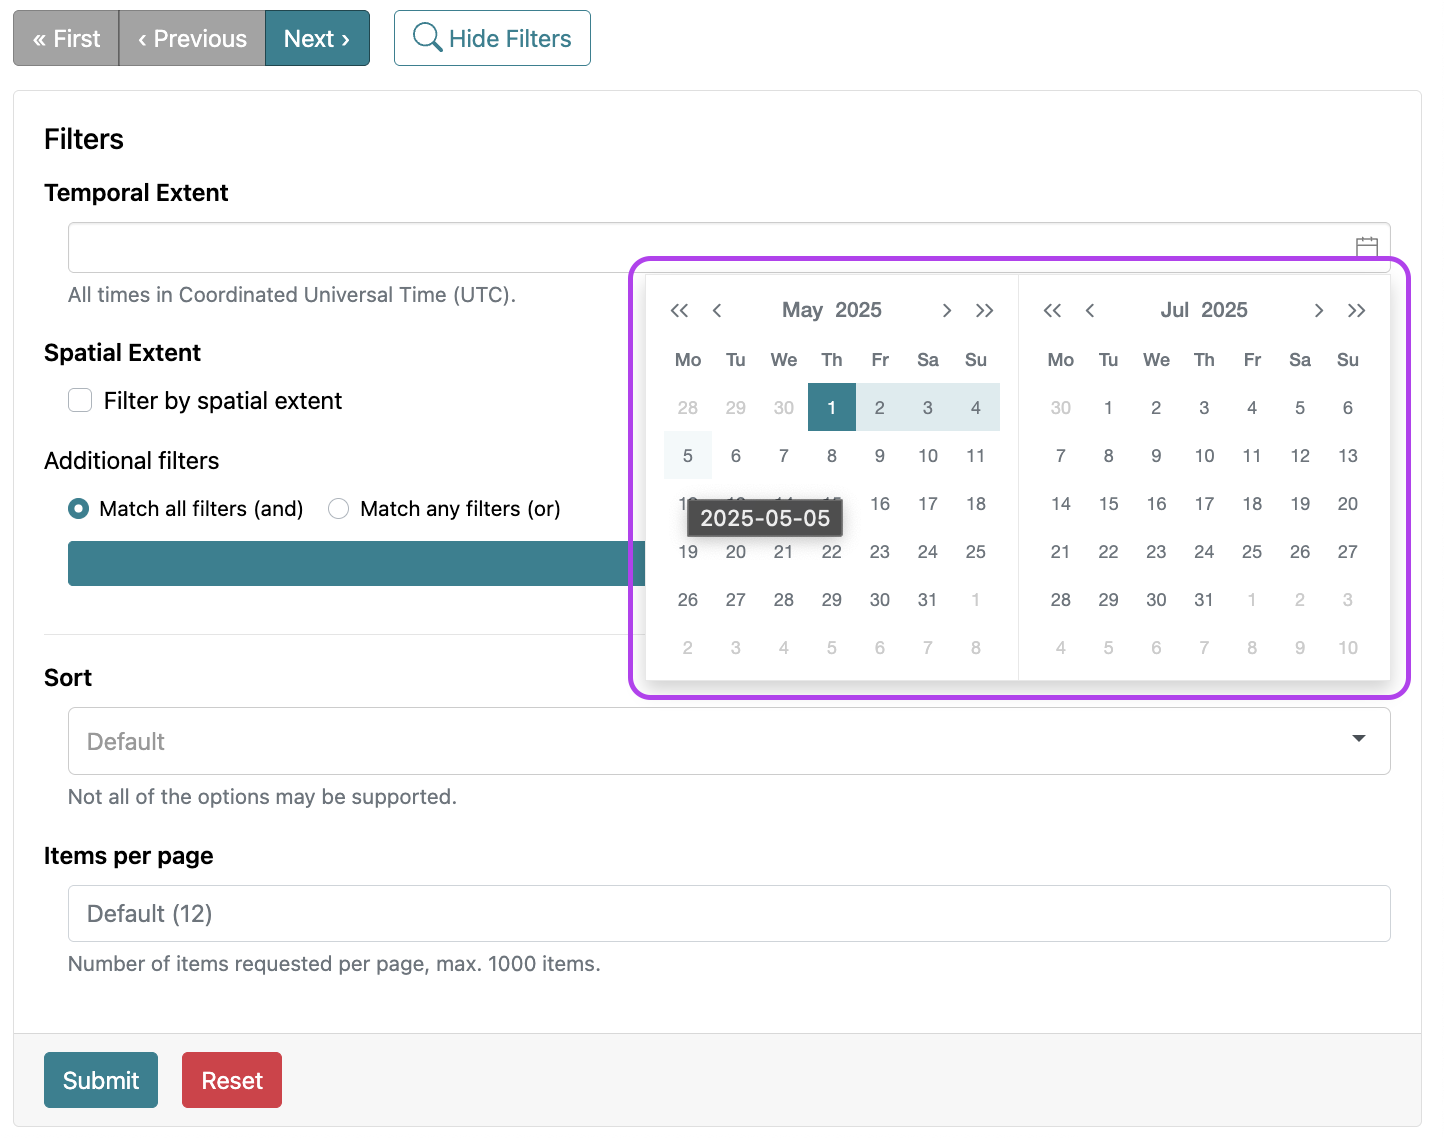
\includegraphics[keepaspectratio]{img/temporal_filter.png}}

}

\caption{Filtering over time}

\end{figure}%

Additionally, we can select a location we are interested in by checking
the \textbf{Filter by spatial extent} box. This allows us to refine our
search over an area of interest. Once you tick the box, a map activates
and allows us to draw a bounding box that we can drag and drop. Let us
select Europe as our area of interest.

\begin{figure}[H]

{\centering \pandocbounded{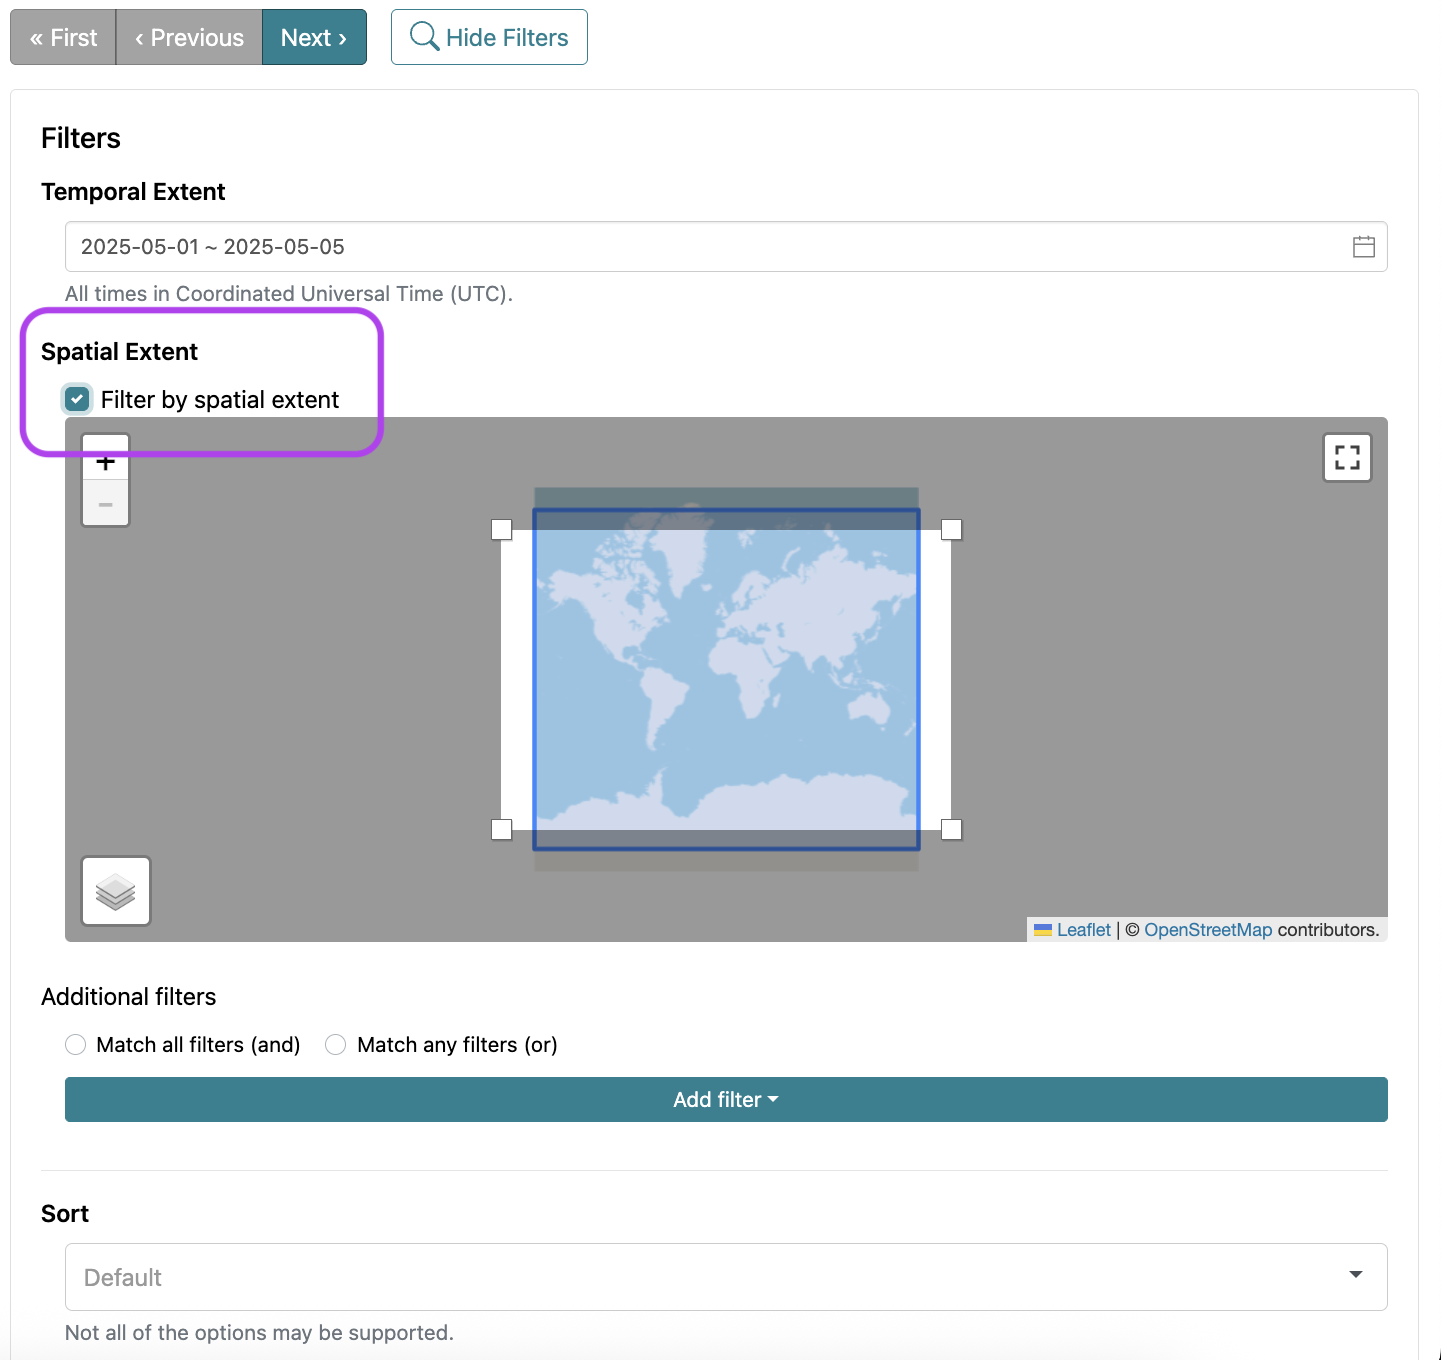
\includegraphics[keepaspectratio]{img/spatial_filter.png}}

}

\caption{Filtering over spatial extent}

\end{figure}%

Once we select the desired time period and area via the filters, we can
sort the items that match our search by ID, Date and Time, or select the
number of resulting items we are interested in per page In this case, we
select 2, so the overview is digestible. Then, we click \textbf{Submit}.

\begin{figure}[H]

{\centering \pandocbounded{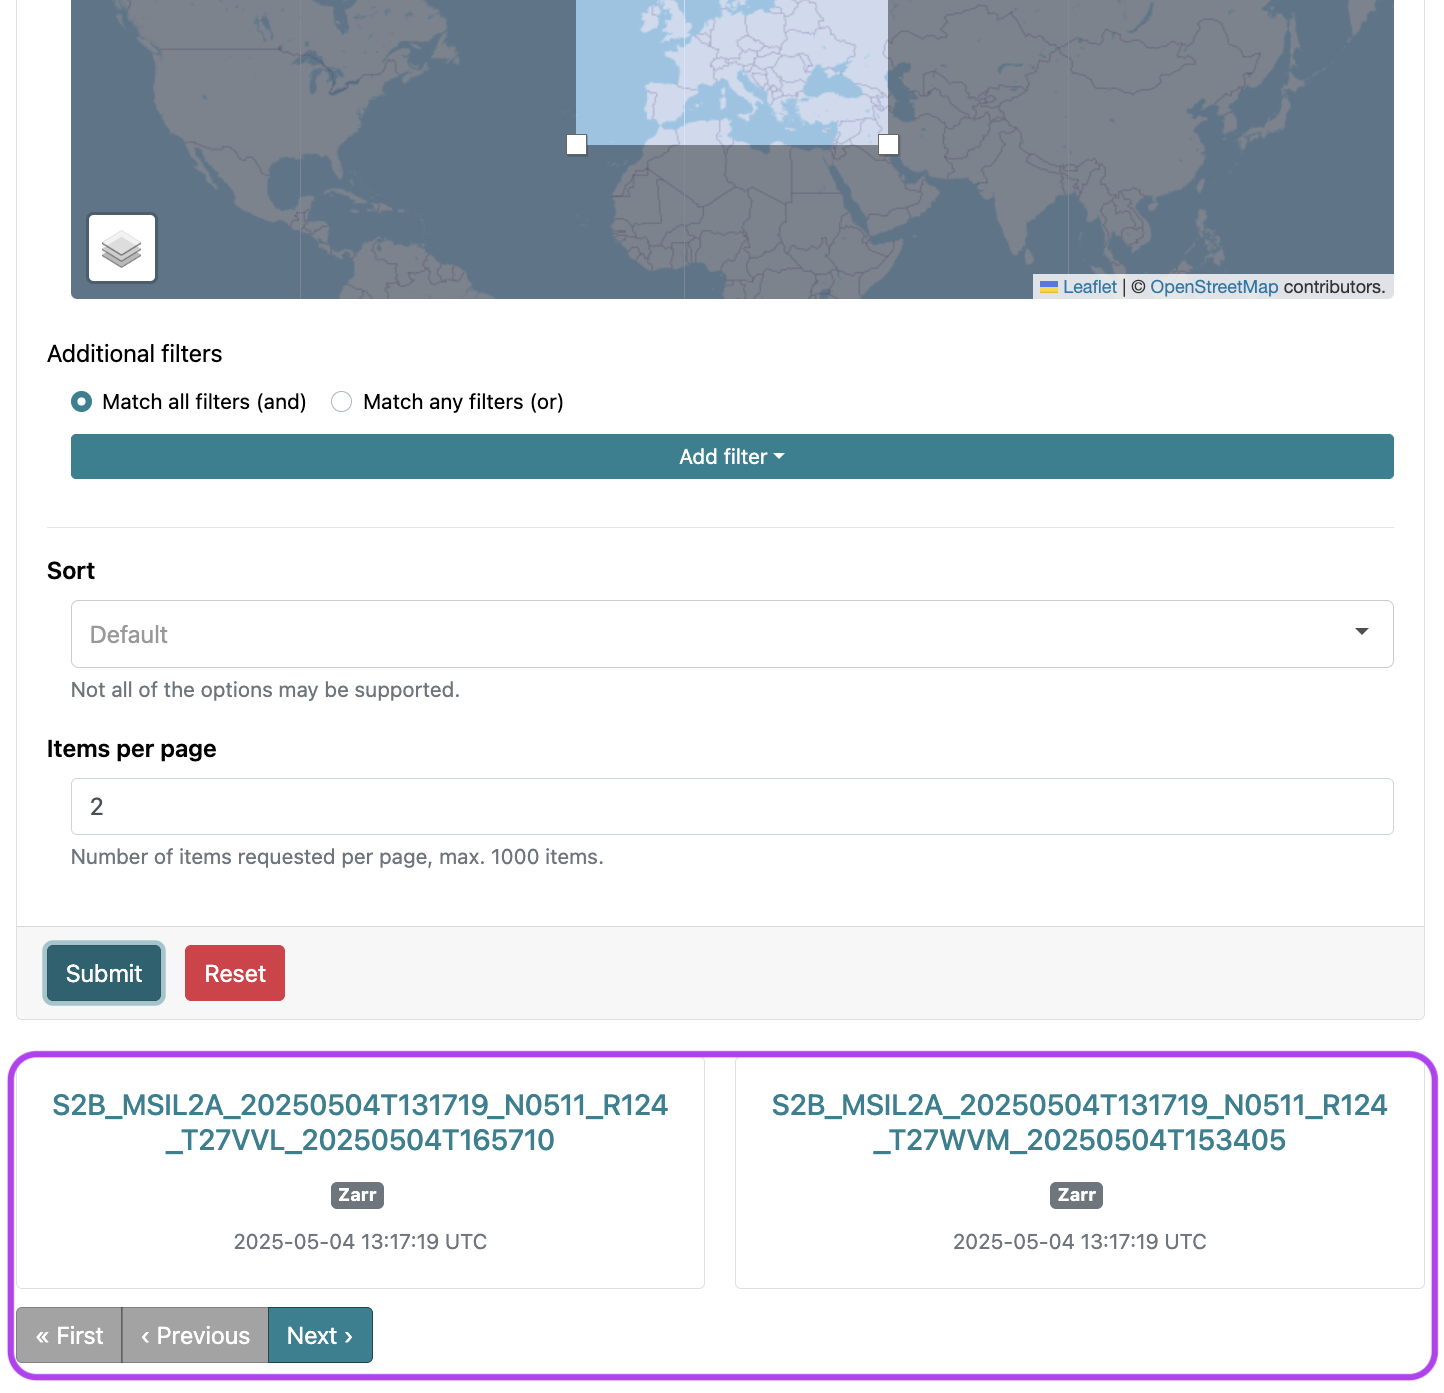
\includegraphics[keepaspectratio]{img/filtered_results.png}}

}

\caption{Resulting Items}

\end{figure}%

Under the window, we can see now that two items appear. For example:
\texttt{S2B\_MSIL2A\_20250504T131719\_N0511\_R124\_T27VVL\_20250504T165710}

We can select any of the resulting items, and this will enable us to
access an \texttt{Item} inside the \texttt{Collection}.

\section{Exploring Items}\label{exploring-items}

When a specific \texttt{Item} sparks our interest, clicking on it will
bring us to detailed overview page for that selected \texttt{Item}.

This \texttt{Item} interface is composed of:

\begin{enumerate}
\def\labelenumi{\arabic{enumi}.}
\tightlist
\item
  \textbf{Description}: The name of the \texttt{Item}. Depending on the
  mission and collection it belongs to, the composition of the name
  changes.
\item
  \textbf{Spatial Extent}: The geographical footprint of the selected
  \texttt{Item} is shown on the map.
\item
  \textbf{Collection Metadata}: A general overview of the Collection's
  metadata, its providers, instruments, resolution, grid and the
  corresponding DOIs for research.
\item
  \textbf{API and URL}: Allows the entry point for further retrieval of
  the individual assets.
\item
  \textbf{Assets menu}: lists all the \texttt{Assets} that are part of
  the selected \texttt{Item}.
\end{enumerate}

\begin{figure}[H]

{\centering \pandocbounded{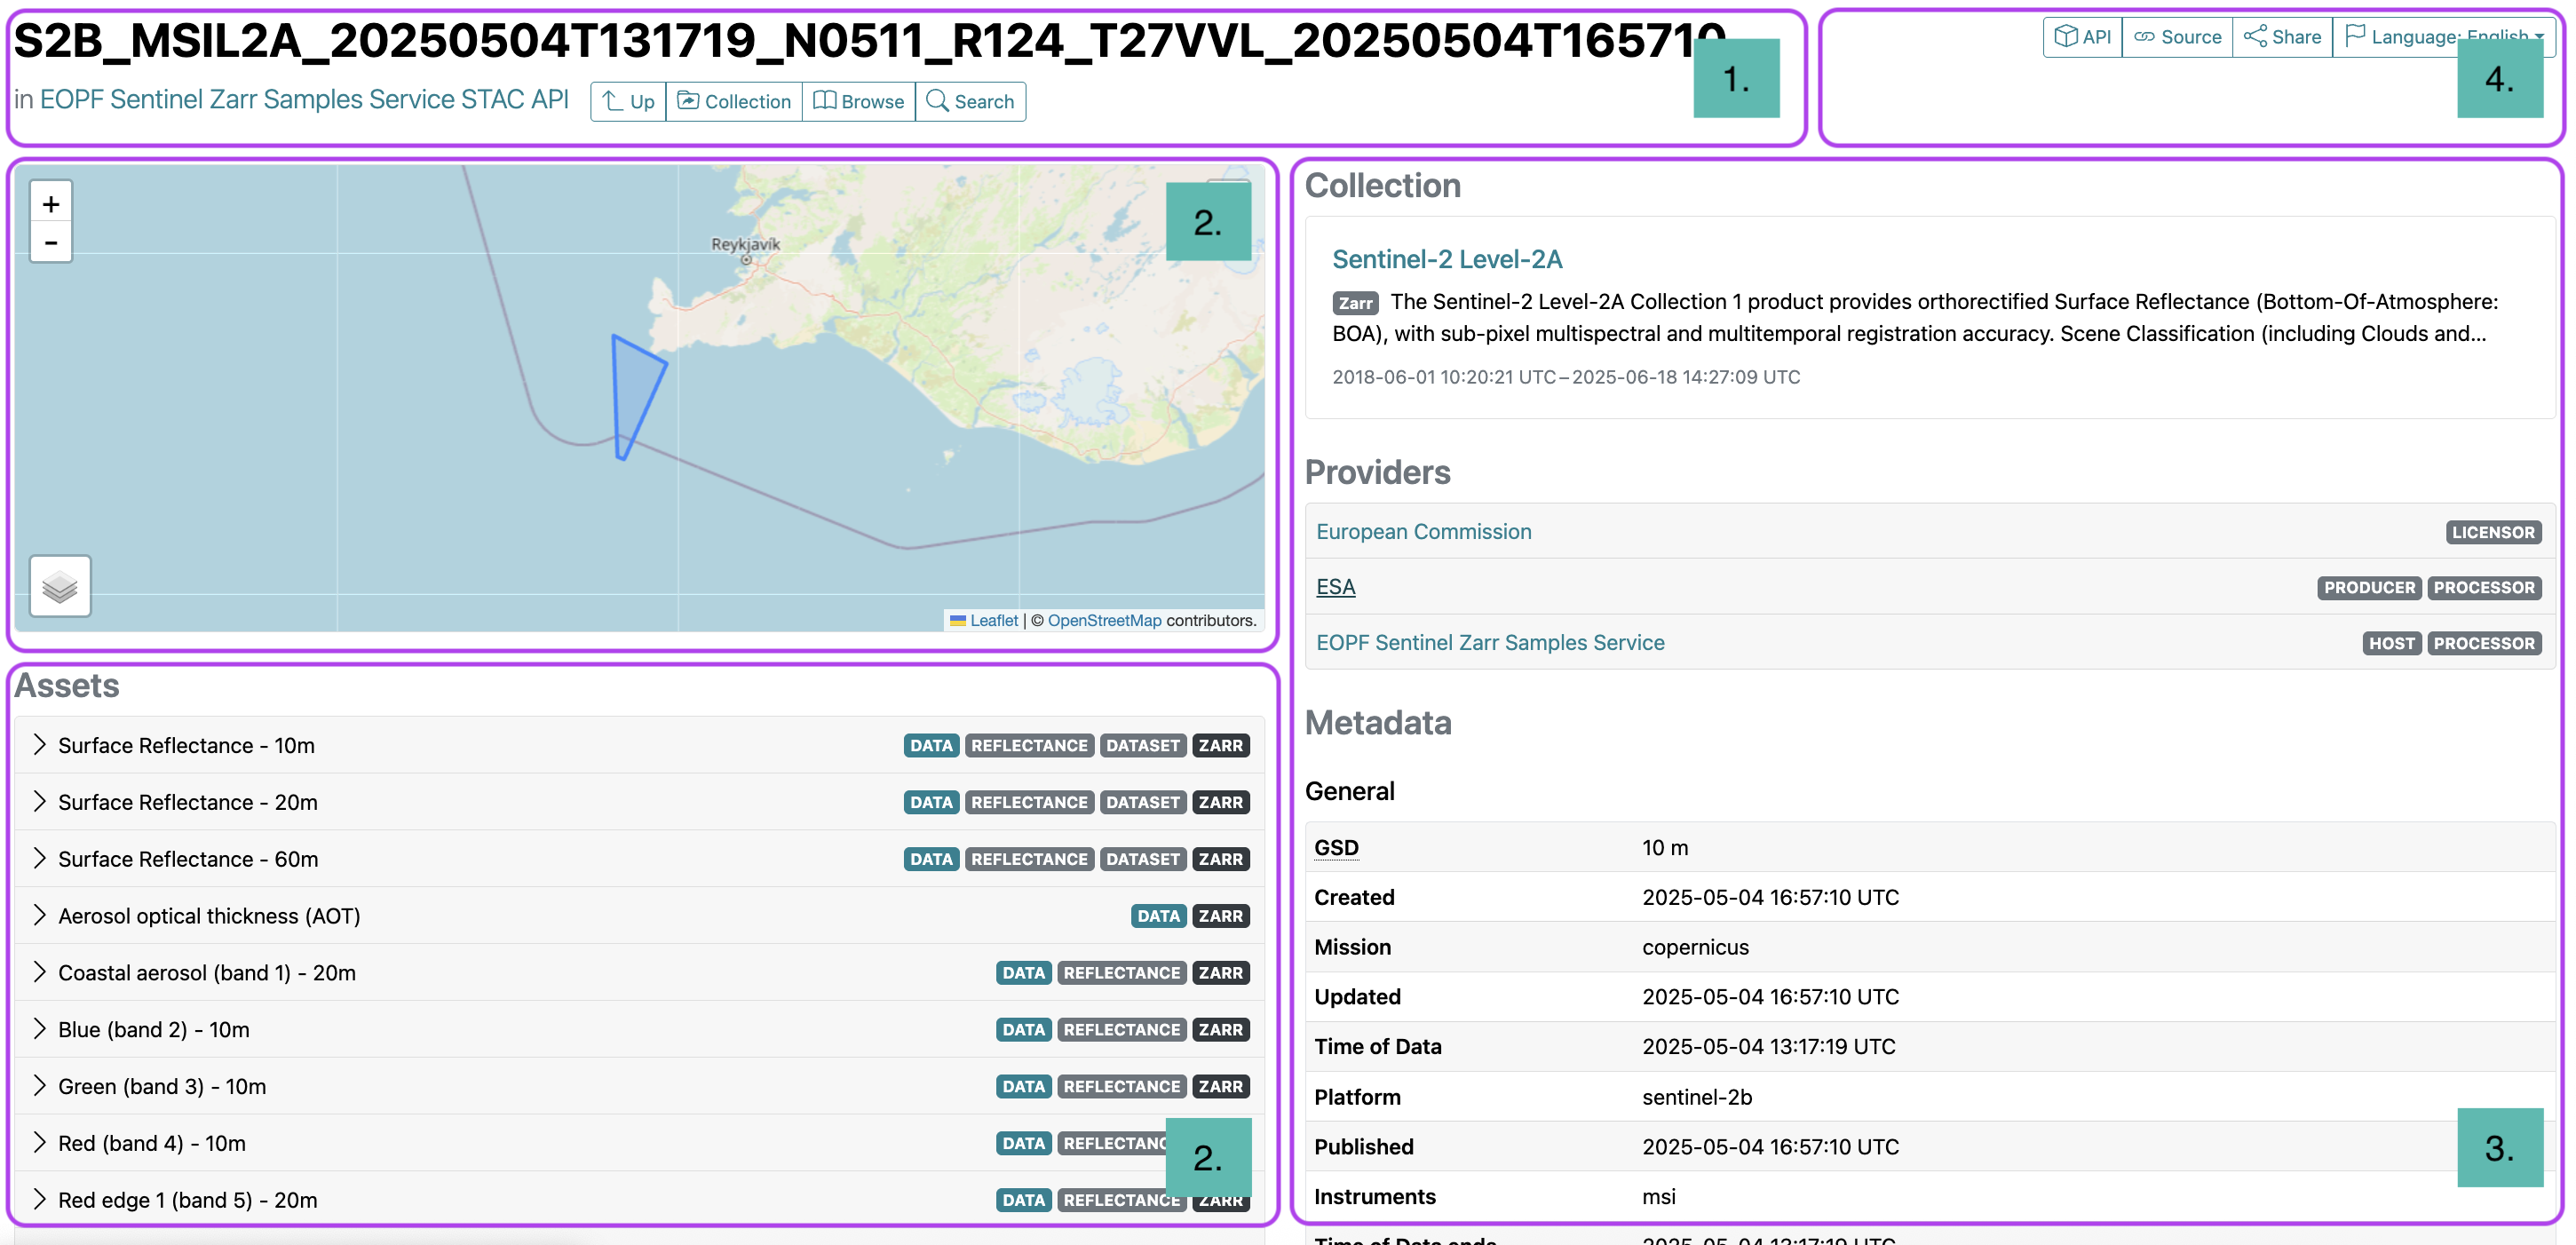
\includegraphics[keepaspectratio]{img/item_des.png}}

}

\caption{The item selected inside the Sentinel-2 Level-2A Collection}

\end{figure}%

\begin{tcolorbox}[enhanced jigsaw, coltitle=black, colback=white, leftrule=.75mm, colbacktitle=quarto-callout-important-color!10!white, titlerule=0mm, title=\textcolor{quarto-callout-important-color}{\faExclamation}\hspace{0.5em}{Important}, rightrule=.15mm, bottomrule=.15mm, bottomtitle=1mm, toptitle=1mm, arc=.35mm, toprule=.15mm, left=2mm, opacityback=0, colframe=quarto-callout-important-color-frame, opacitybacktitle=0.6, breakable]

At this level of the STAC structure, we are already diving deep into the
STAC levels, and have explored the \texttt{Catalog}, \texttt{Collection}
and \texttt{Item} components described in the
\hyperref[introduction-to-stac]{Introduction to STAC} section.

\end{tcolorbox}

\section{Assets}\label{assets}

Inside the selected \texttt{Item}, we will get an overview of the
available \texttt{Assets} that belong to the \texttt{Item}. By expanding
the \textbf{dropdown menu} for any \texttt{Asset} of interest, you can
access its specific metadata and most importantly, the actual data.

\begin{figure}[H]

{\centering \pandocbounded{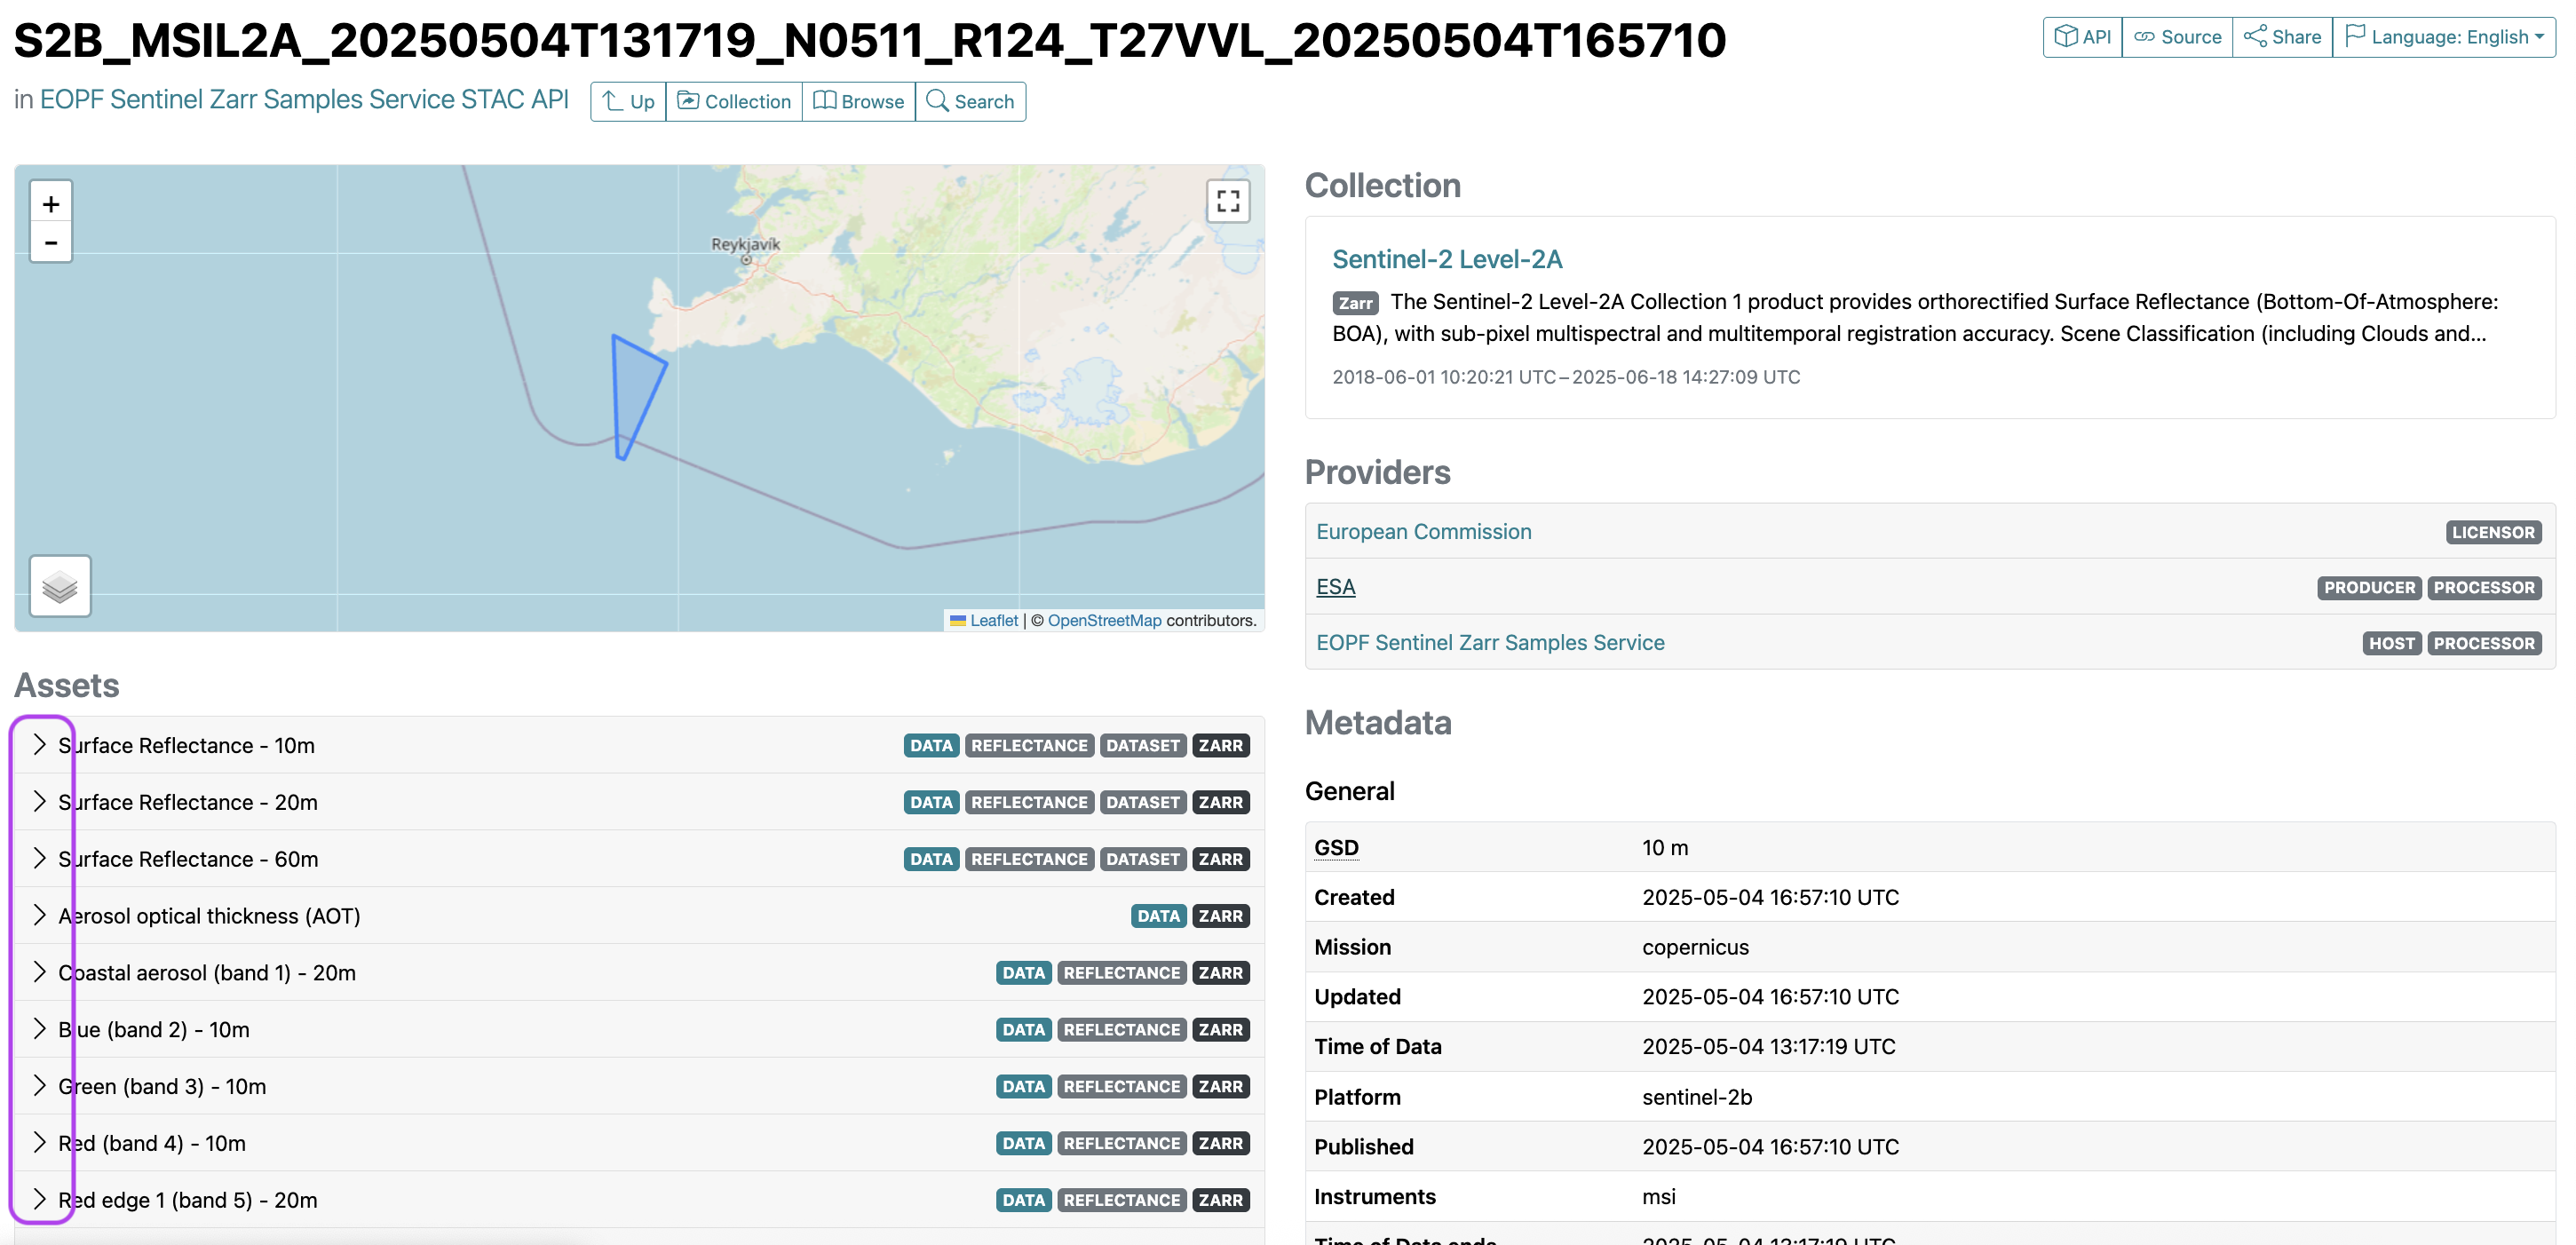
\includegraphics[keepaspectratio]{img/drop_down.png}}

}

\caption{Overview of the web interface on Asset level}

\end{figure}%

In the case of the \textbf{Sentinel-2 Level-2A} collection, each asset
corresponds to one of the 13 spectral bands available. The array
information provides details about the structure and content of the
data, hinting at the actual values contained within the asset. It also
contains the chunking grid specification and all the crucial metadata
necessary to structure and process the data through a wide range of
geospatial methodologies.

\subsection{Accessing Assets}\label{accessing-assets}

For direct data access of \texttt{Assetz} and therefore the actual data,
there are two options provided via the web interface: *
\textbf{Download}: It is possible to download only one asset separately
in \texttt{.zarr} format by clicking the \emph{Download} option
associated with an Asset, and * \textbf{Copy URL}: We can also retrieve
the the unique URL of the specified \texttt{Asset}, which allows us
directly integrating the link into programmatic workflows, wihthout the
need to download the \texttt{Asset}. We can get it by simply clicking on
the \emph{Copy URL} option under the \texttt{Asset} of our interest.

\begin{figure}[H]

{\centering \pandocbounded{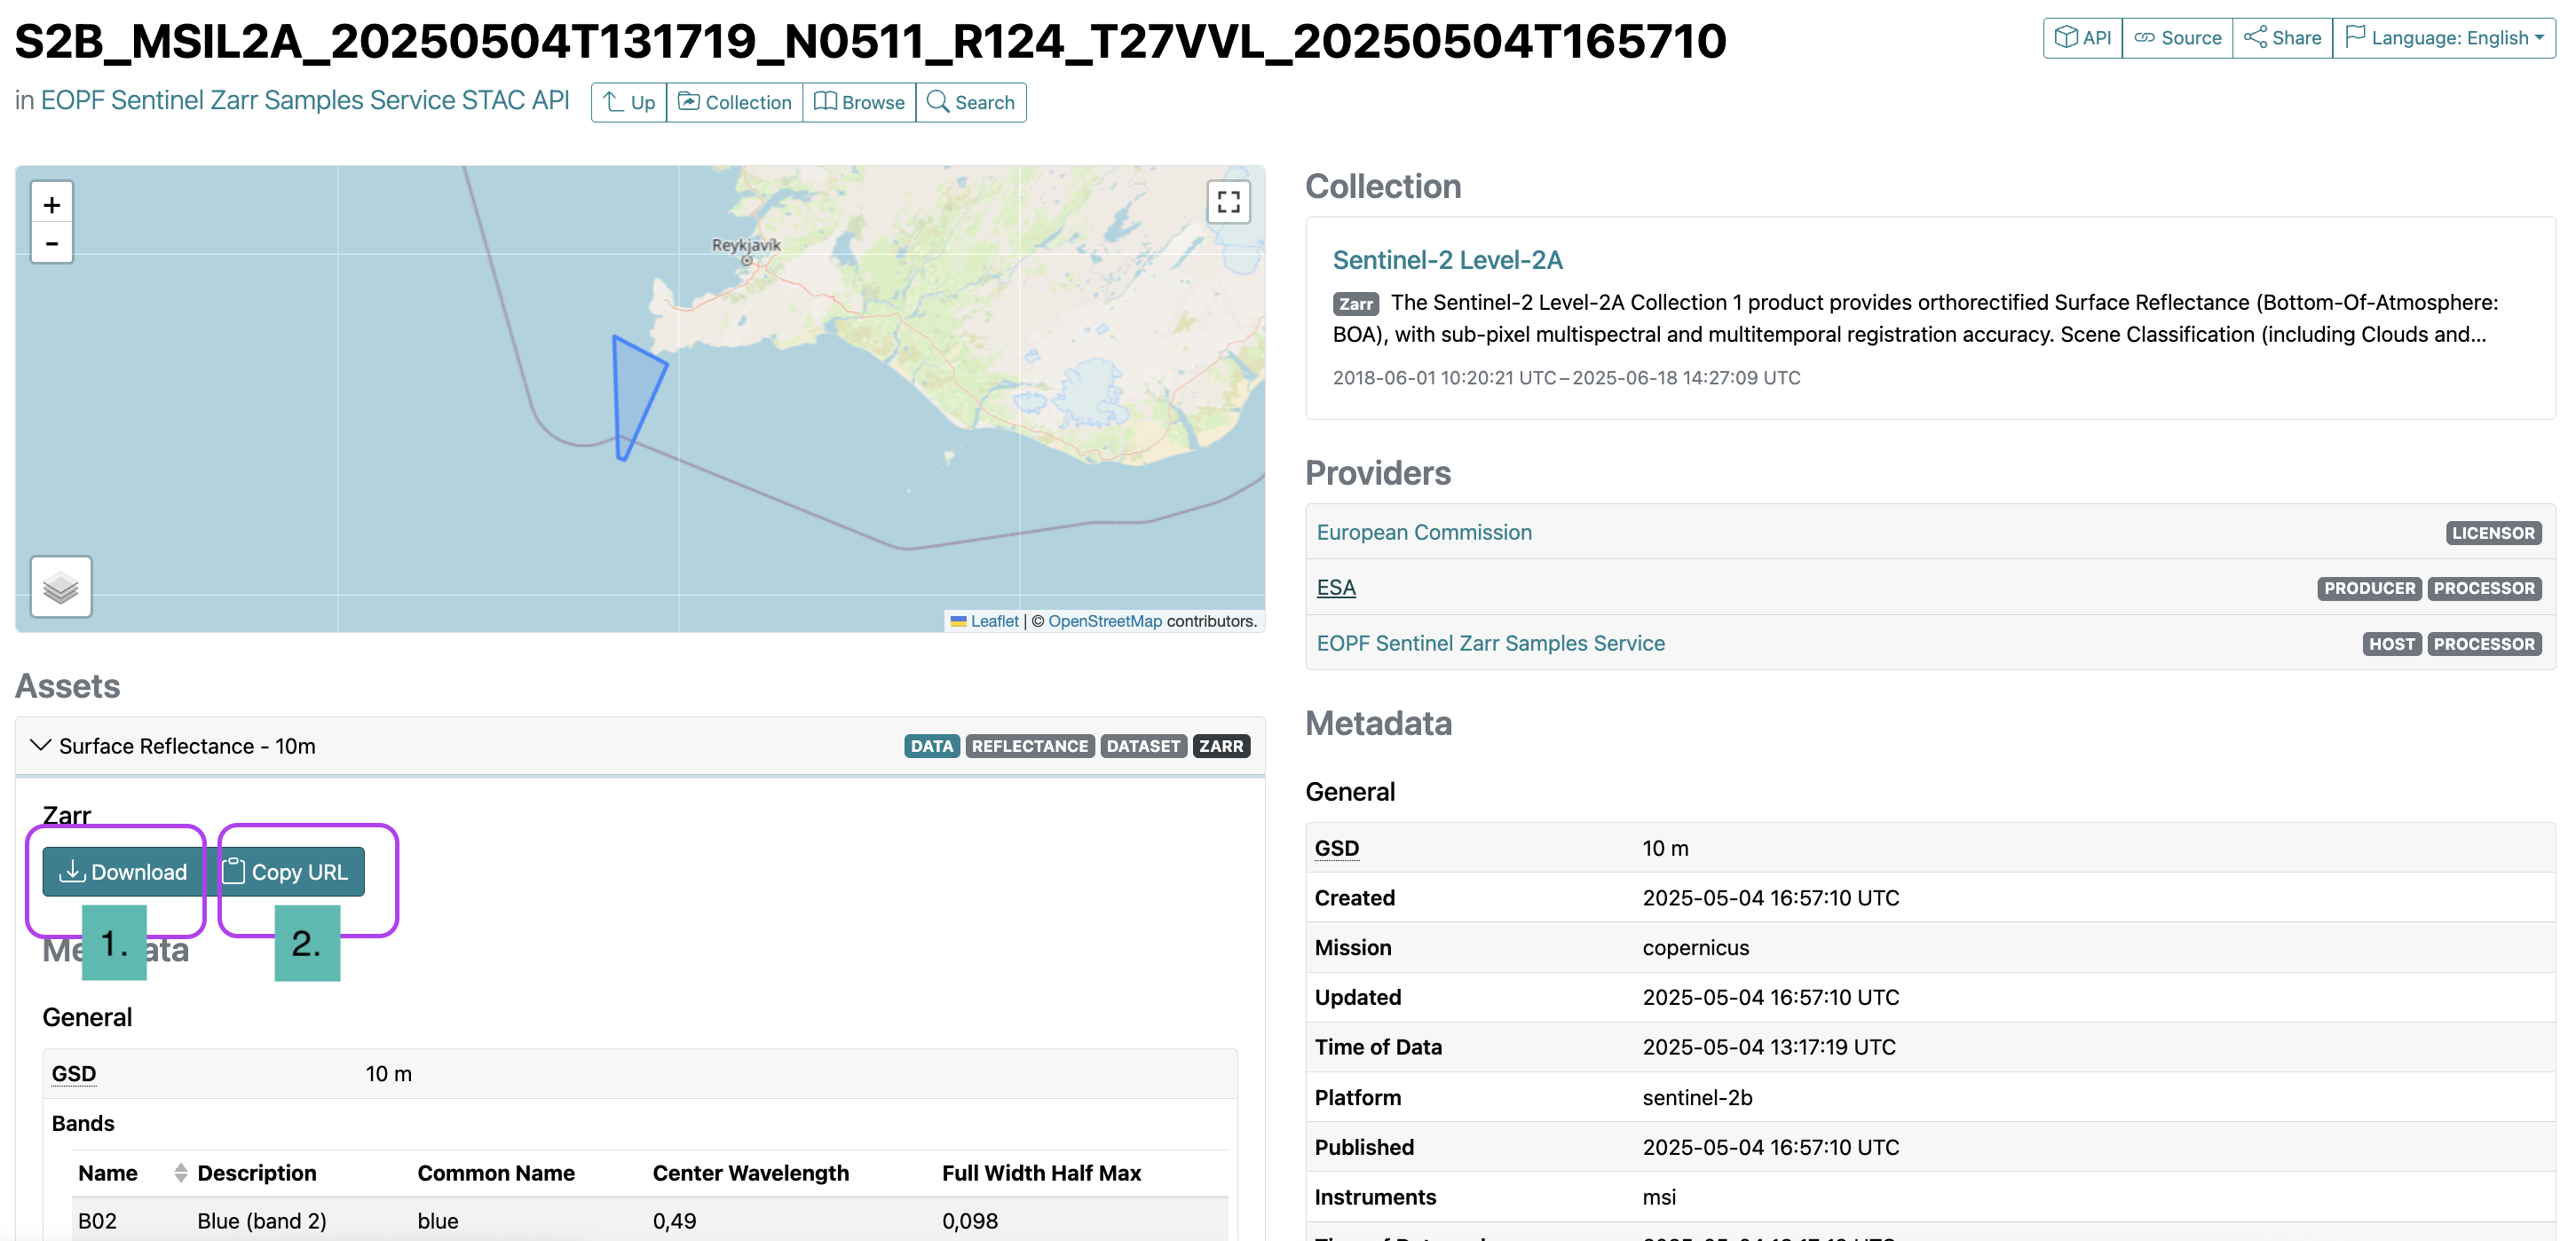
\includegraphics[keepaspectratio]{img/download_img.png}}

}

\caption{Data access options via the web interface}

\end{figure}%

\section{💪 Now it is your turn}\label{now-it-is-your-turn-1}

Your task now is to explore the web interface of the
\href{https://stac.browser.user.eopf.eodc.eu/?.language=en}{EOPF
Sentinel Zarr Samples Service STAC Catalog} on your own and explore
other \texttt{Collections} than the one we showcased.

\subsection{Task 1: Discover Sentinel-1 GRD
Data}\label{task-1-discover-sentinel-1-grd-data}

Navigate to the
\href{https://stac.browser.user.eopf.eodc.eu/collections/sentinel-1-l1-grd?.itemFilterOpen=1&language=en}{Sentinel-1
Level-1 GRD Collection}.

\begin{itemize}
\tightlist
\item
  How many items can you find for the most recent two years available in
  the catalog?
\item
  Try filtering by different time periods and observe how the results
  change. How many items are available for September 2023?
\end{itemize}

\subsection{Task 2: Mapping Your
Interests}\label{task-2-mapping-your-interests}

Explore the interactive map within the
\href{https://stac.browser.user.eopf.eodc.eu/collections/sentinel-1-l1-grd?.itemFilterOpen=1&language=en}{Sentinel-1
Level-1 GRD} and the
\href{https://stac.browser.user.eopf.eodc.eu/collections/sentinel-2-l2a?.language=en}{Sentinel-2
Level-2A} collections.

\begin{itemize}
\tightlist
\item
  Can you identify and list the names of at least three distinct
  geographical areas where a significant number of items are available?
  (Hint: Look for clusters of the displayed items!)
\end{itemize}

\subsection{Task 3: Unpacking an Asset}\label{task-3-unpacking-an-asset}

Select an item from any collection that looks interesting to you. Click
on it to view its details. Then, expand one of the assets.

\begin{itemize}
\tightlist
\item
  What kind of array information is provided?
\item
  Who is the data provider?
\item
  How would this information be useful if you were to process this data?
\end{itemize}

\section{Conclusion}\label{conclusion-6}

This section walked you through the web interface of the
\href{https://stac.browser.user.eopf.eodc.eu/?.language=en}{EOPF
Sentinel Zarr Samples Service STAC Catalog}. We have demonstrated how to
navigate its interface, from the initial overview of the available
\texttt{Collections} to the detailed inspection of specific
\texttt{Items} and \texttt{Asset}. By understanding the structure and
components of a STAC catalog, we are able to efficiently access
re-engineered EOPF Zarr assets.

\section{What's next?}\label{whats-next-6}

In the next \href{./33_eopf_stac_connection.ipynb}{section}, we will
explore how to programmatically connect to and search through the EOPF
Sentinel Zarr Samples Service STAC API with the help of the
\texttt{pystac} and the \texttt{pystac-client} Python libraries.

\chapter{Access the EOPF Zarr STAC API with
Python}\label{access-the-eopf-zarr-stac-api-with-python}

\subsection{Introduction}\label{introduction-7}

In this section, we will dive into the programmatic access of EOPF Zarr
Collections available in the
\href{https://stac.browser.user.eopf.eodc.eu/?.language=en}{EOPF
Sentinel Zarr Sample Service STAC Catalog}. We will introduce Python
libraries enable us to effectively access and search through STAC
catalogs.

\subsection{What we will learn}\label{what-we-will-learn-6}

\begin{itemize}
\tightlist
\item
  🔍 How to \textbf{programmatically browse} through available
  collections availalbe via the EOPF Zarr STAC API
\item
  📊 Understanding \textbf{collection metadata} in user-friendly terms
\item
  🎯 \textbf{Searching for specific data} with help of the
  \texttt{pystac} and \texttt{pystac-client} libraries.
\end{itemize}

\subsection{Prerequisites}\label{prerequisites-1}

For this tutorial, we will make use of the
\href{https://pystac.readthedocs.io/en/stable/}{pystac} and
\href{https://pystac-client.readthedocs.io/en/latest/api.html}{pystac\_client}
Python libraries that facilitate the programmatic access and efficient
search of a STAC Catalog.

\subsubsection{Import libraries}\label{import-libraries-1}

\begin{Shaded}
\begin{Highlighting}[]
\ImportTok{import}\NormalTok{ requests}
\ImportTok{from}\NormalTok{ typing }\ImportTok{import}\NormalTok{ List, Optional, cast}
\ImportTok{from}\NormalTok{ pystac }\ImportTok{import}\NormalTok{ Collection, MediaType}
\ImportTok{from}\NormalTok{ pystac\_client }\ImportTok{import}\NormalTok{ Client, CollectionClient}
\ImportTok{from}\NormalTok{ datetime }\ImportTok{import}\NormalTok{ datetime}
\end{Highlighting}
\end{Shaded}

\subsubsection{Helper functions}\label{helper-functions-1}

\paragraph{\texorpdfstring{\texttt{list\_found\_elements}}{list\_found\_elements}}\label{list_found_elements}

As we are expecting to visualise several elements that will be stored in
lists, we define a function that will allow us retrieve item
\texttt{id}'s and collections \texttt{id}'s for further retrieval.

\begin{Shaded}
\begin{Highlighting}[]
\KeywordTok{def}\NormalTok{ list\_found\_elements(search\_result):}
    \BuiltInTok{id} \OperatorTok{=}\NormalTok{ []}
\NormalTok{    coll }\OperatorTok{=}\NormalTok{ []}
    \ControlFlowTok{for}\NormalTok{ item }\KeywordTok{in}\NormalTok{ search\_result.items(): }\CommentTok{\#retrieves the result inside the catalogue.}
        \BuiltInTok{id}\NormalTok{.append(item.}\BuiltInTok{id}\NormalTok{)}
\NormalTok{        coll.append(item.collection\_id)}
    \ControlFlowTok{return} \BuiltInTok{id}\NormalTok{ , coll}
\end{Highlighting}
\end{Shaded}

\section{Establish a connection to the EOPF Zarr STAC
Catalog}\label{establish-a-connection-to-the-eopf-zarr-stac-catalog}

Our first step is to establish a connection to the EOPF Sentinel Zarr
Sample Service STAC Catalog. For this, you need the Catalog's base URL,
which you can find on the web interface under the \textbf{API \& URL}
tab. By clicking on 🔗\textbf{Source}, you will get the address of the
STAC metadata file - which is availabl
\href{https://stac.core.eopf.eodc.eu/}{here}.

\begin{figure}[H]

{\centering \pandocbounded{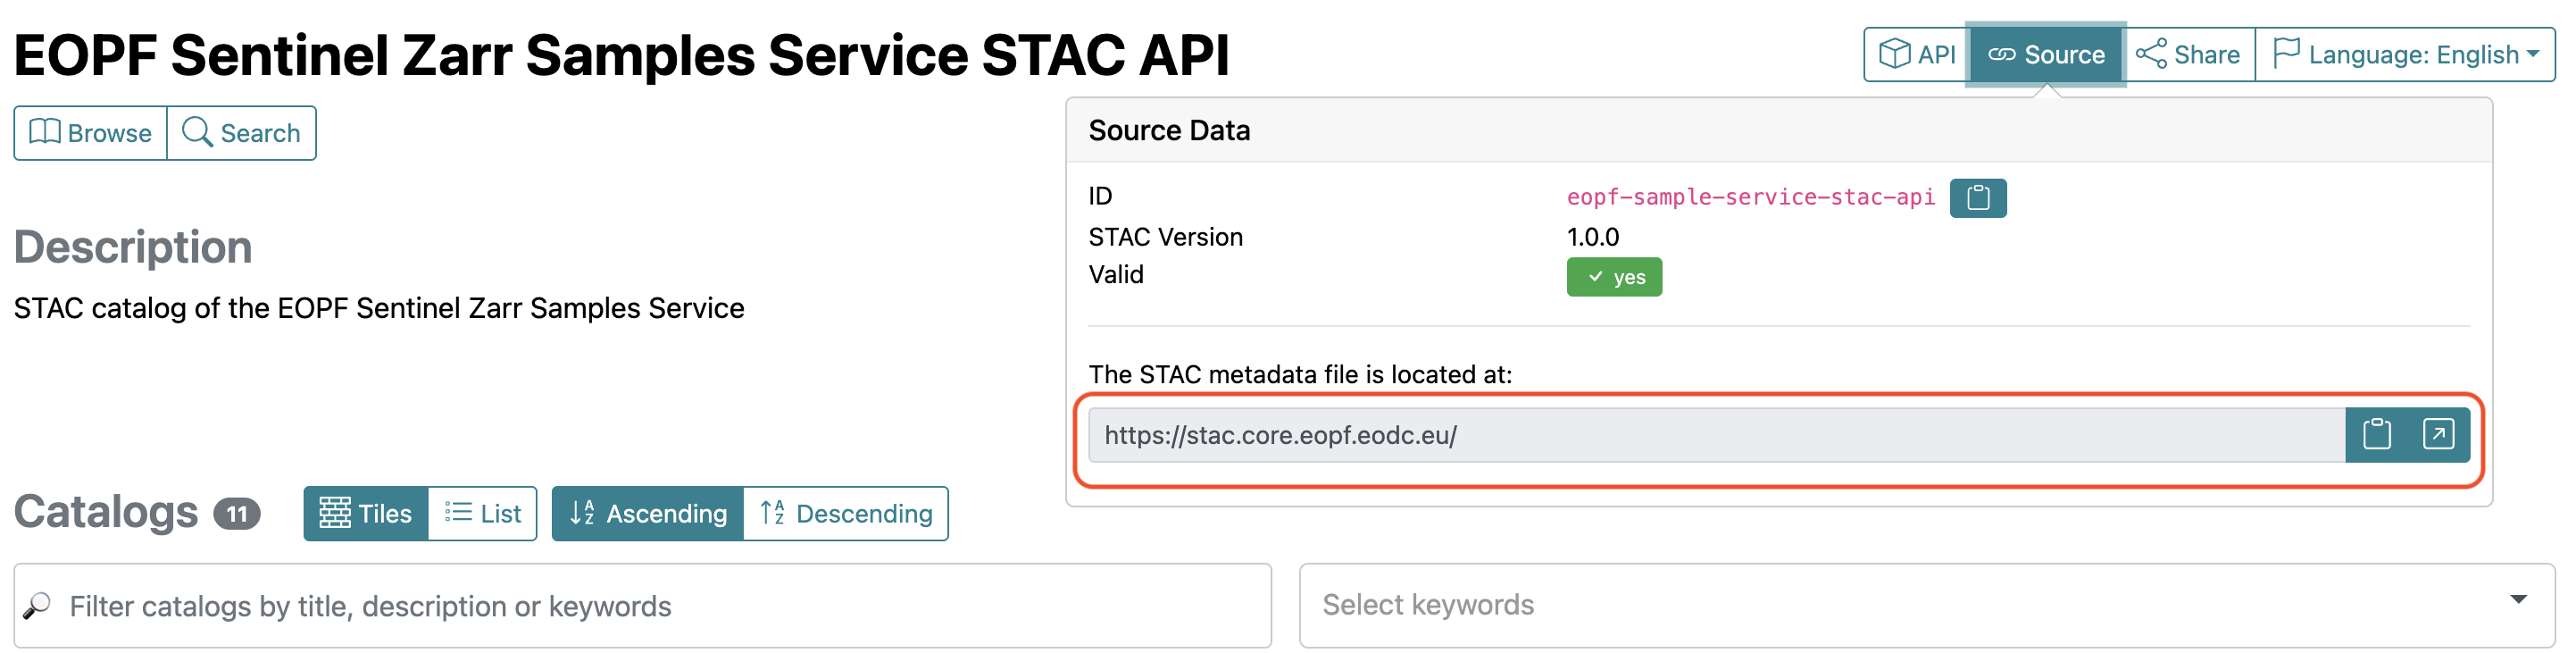
\includegraphics[keepaspectratio]{img/api_connection.png}}

}

\caption{EOPF API url for connection}

\end{figure}%

Copy paste the URL: \texttt{https://stac.core.eopf.eodc.eu/}.

With the \texttt{Client.open()} function, we can create the access to
the starting point of the Catalog by providing the specific url. If the
connection was successful, you will see the description of the STAC
catalog and additional information.

\begin{Shaded}
\begin{Highlighting}[]
\NormalTok{eopf\_stac\_api\_root\_endpoint }\OperatorTok{=} \StringTok{"https://stac.core.eopf.eodc.eu/"} \CommentTok{\#root starting point}
\NormalTok{eopf\_catalog }\OperatorTok{=}\NormalTok{ Client.}\BuiltInTok{open}\NormalTok{(url}\OperatorTok{=}\NormalTok{eopf\_stac\_api\_root\_endpoint) }\CommentTok{\# calls the selected url}
\NormalTok{eopf\_catalog}
\end{Highlighting}
\end{Shaded}

\begin{verbatim}
<Client id=eopf-sample-service-stac-api>
\end{verbatim}

Congratulations. We successfully connected to the EOPF Zarr STAC Catalog
and we can now start exploring its content.

\section{Explore available
collections}\label{explore-available-collections}

Once a connection established, the next logical step is to get an
overview of all the collections the STAC catalog offers. We can do this
with the function \texttt{get\_all\_collections()}. The result is a
list, which we can loop through to print the relevant collection IDs.

\textbf{Please note:} Since the EOPF Zarr STAC Catalog is still in
active development, we need to test whether a collection is valid,
otherwise you might get an error message. The code below is testing for
validity and for one collection, it throws an error.

You see, that so far, we can browse through 10 available collections

\begin{Shaded}
\begin{Highlighting}[]
\ControlFlowTok{try}\NormalTok{:}
    \ControlFlowTok{for}\NormalTok{ collection }\KeywordTok{in}\NormalTok{ eopf\_catalog.get\_all\_collections():}
        \BuiltInTok{print}\NormalTok{(collection.}\BuiltInTok{id}\NormalTok{)}

\ControlFlowTok{except} \PreprocessorTok{Exception}\NormalTok{:}
    \BuiltInTok{print}\NormalTok{(}
        \StringTok{"* [https://github.com/EOPF{-}Sample{-}Service/eopf{-}stac/issues/18 appears to not be resolved]"}
\NormalTok{    )}
\end{Highlighting}
\end{Shaded}

\begin{verbatim}
sentinel-2-l2a
sentinel-3-slstr-l1-rbt
sentinel-3-olci-l2-lfr
sentinel-2-l1c
sentinel-3-slstr-l2-lst
sentinel-1-l1-slc
sentinel-3-olci-l1-efr
sentinel-3-olci-l1-err
sentinel-1-l2-ocn
sentinel-1-l1-grd
* [https://github.com/EOPF-Sample-Service/eopf-stac/issues/18 appears to not be resolved]
\end{verbatim}

In a next step, we can select one \texttt{collection} and retrieve
certain metadata that allow us to get more information about the
selected collection, such as keywords, the ID and useful links for
resources.

\begin{Shaded}
\begin{Highlighting}[]
\NormalTok{S2l2a\_coll }\OperatorTok{=}\NormalTok{ eopf\_catalog.get\_collection(}\StringTok{\textquotesingle{}sentinel{-}2{-}l2a\textquotesingle{}}\NormalTok{)}
\BuiltInTok{print}\NormalTok{(}\StringTok{\textquotesingle{}Keywords:        \textquotesingle{}}\NormalTok{,S2l2a\_coll.keywords)}
\BuiltInTok{print}\NormalTok{(}\StringTok{\textquotesingle{}Catalog ID:      \textquotesingle{}}\NormalTok{,S2l2a\_coll.}\BuiltInTok{id}\NormalTok{)}
\BuiltInTok{print}\NormalTok{(}\StringTok{\textquotesingle{}Available Links: \textquotesingle{}}\NormalTok{,S2l2a\_coll.links)}
\end{Highlighting}
\end{Shaded}

\begin{verbatim}
Keywords:         ['Copernicus', 'Sentinel', 'EU', 'ESA', 'Satellite', 'Global', 'Imagery', 'Reflectance']
Catalog ID:       sentinel-2-l2a
Available Links:  [<Link rel=items target=https://stac.core.eopf.eodc.eu/collections/sentinel-2-l2a/items>, <Link rel=parent target=https://stac.core.eopf.eodc.eu/>, <Link rel=root target=<Client id=eopf-sample-service-stac-api>>, <Link rel=self target=https://stac.core.eopf.eodc.eu/collections/sentinel-2-l2a>, <Link rel=license target=https://sentinel.esa.int/documents/247904/690755/Sentinel_Data_Legal_Notice>, <Link rel=cite-as target=https://doi.org/10.5270/S2_-znk9xsj>, <Link rel=http://www.opengis.net/def/rel/ogc/1.0/queryables target=https://stac.core.eopf.eodc.eu/collections/sentinel-2-l2a/queryables>]
\end{verbatim}

\section{Searching inside the EOPF STAC
API}\label{searching-inside-the-eopf-stac-api}

With the \texttt{.search()} function of the \texttt{pystac-client}
library, we can search inside a STAC catalog we established a connection
with. We can filter based on a series of parameters to tailor the search
for available data for a specific time period and geographic bounding
box.

\subsection{Filter for temporal
extent}\label{filter-for-temporal-extent}

Let us search on the \texttt{datetime} parameter. For this, we specify
the \texttt{datetime} argument for a time period we are interested in,
e.g.~from 1 May 2020 to 31 May 2023. In addition, we also specify the
\texttt{collection} parameter indicating that we only want to search for
the Sentinel-2 L2A collection.

We apply the helper function \texttt{list\_found\_elements} which
constructs a list from the search result. If we check the length of the
final list, we can see that for the specified time period, 196 items
were found.

\begin{Shaded}
\begin{Highlighting}[]
\NormalTok{time\_frame }\OperatorTok{=}\NormalTok{ eopf\_catalog.search(  }\CommentTok{\#searching the catalog}
\NormalTok{    collections}\OperatorTok{=}\StringTok{\textquotesingle{}sentinel{-}2{-}l2a\textquotesingle{}}\NormalTok{,}
\NormalTok{    datetime}\OperatorTok{=}\StringTok{"2020{-}05{-}01T00:00:00Z/2023{-}05{-}31T23:59:59.999999Z"}\NormalTok{)  }\CommentTok{\# the interval we are interested in, separated by \textquotesingle{}/\textquotesingle{}}

\CommentTok{\# we apply the helper function \textasciigrave{}list\_found\_elements\textasciigrave{}}
\NormalTok{time\_items}\OperatorTok{=}\NormalTok{list\_found\_elements(time\_frame)}
\BuiltInTok{print}\NormalTok{(time\_frame)}

\BuiltInTok{print}\NormalTok{(}\StringTok{"Search Results:"}\NormalTok{)}
\BuiltInTok{print}\NormalTok{(}\StringTok{\textquotesingle{}Total Items Found for Sentinel{-}2 L{-}2A between May 1, 2020, and May 31, 2023:  \textquotesingle{}}\NormalTok{,}\BuiltInTok{len}\NormalTok{(time\_items[}\DecValTok{0}\NormalTok{]))}
\end{Highlighting}
\end{Shaded}

\begin{verbatim}
<pystac_client.item_search.ItemSearch object at 0x705b9a4b3130>
Search Results:
Total Items Found for Sentinel-2 L-2A between May 1, 2020, and May 31, 2023:   196
\end{verbatim}

\subsection{Filter for spatial extent}\label{filter-for-spatial-extent}

Now, let us filter based on a specific area of interest. We can use the
\texttt{bbox} argument, which is composed by providing the top-left and
bottom-right corner coordinates. It is similar to drawing the extent in
the interactive map of the EOPF browser interface.

For example, we defined a bounding box of the outskirts of Innsbruck,
Austria. We then again apply the helper funnction
\texttt{list\_found\_elements} and see that for the defined area, only
39 items are available.

\begin{Shaded}
\begin{Highlighting}[]
\NormalTok{bbox\_search }\OperatorTok{=}\NormalTok{  eopf\_catalog.search(  }\CommentTok{\#searching the catalog}
\NormalTok{    collections}\OperatorTok{=}\StringTok{\textquotesingle{}sentinel{-}2{-}l2a\textquotesingle{}}\NormalTok{,}
\NormalTok{    bbox}\OperatorTok{=}\NormalTok{(}
        \FloatTok{11.124756}\NormalTok{, }\FloatTok{47.311058}\NormalTok{, }\CommentTok{\#top left}
        \FloatTok{11.459839}\NormalTok{, }\FloatTok{47.463624}  \CommentTok{\#bottom{-}right}
\NormalTok{        )}
\NormalTok{)}

\NormalTok{innsbruck\_sets}\OperatorTok{=}\NormalTok{list\_found\_elements(bbox\_search) }\CommentTok{\#we apply our constructed function that stores internal information}

\CommentTok{\#Results}
\BuiltInTok{print}\NormalTok{(}\StringTok{"Search Result:"}\NormalTok{)}
\BuiltInTok{print}\NormalTok{(}\StringTok{\textquotesingle{}Total Items Found:  \textquotesingle{}}\NormalTok{,}\BuiltInTok{len}\NormalTok{(innsbruck\_sets[}\DecValTok{0}\NormalTok{]))}
\end{Highlighting}
\end{Shaded}

\begin{verbatim}
Search Result:
Total Items Found:   39
\end{verbatim}

\subsection{Combined filtering: Collection + temporal extent + spatial
extent}\label{combined-filtering-collection-temporal-extent-spatial-extent}

As a usual workflow, we often look for datasets within an AOI and a
specific period of time time. The \texttt{search()} function allows us
also to combine the \texttt{collection}, \texttt{bbox} and
\texttt{datetime} arguments in one search request.

Let us now search for Items available for the AOI aroudn Innsbruck
within the previously defined timeframe for the \textbf{Sentinel-2
Level-2A} collection. As a result, we get 27 Items that are available
for our selection.

\begin{Shaded}
\begin{Highlighting}[]
\NormalTok{innsbruck\_s2 }\OperatorTok{=}\NormalTok{ eopf\_catalog.search( }
\NormalTok{    collections}\OperatorTok{=} \StringTok{\textquotesingle{}sentinel{-}2{-}l2a\textquotesingle{}}\NormalTok{, }\CommentTok{\# interest Collection,}
\NormalTok{    bbox}\OperatorTok{=}\NormalTok{(}\FloatTok{11.124756}\NormalTok{, }\FloatTok{47.311058}\NormalTok{, }\CommentTok{\# AOI extent}
          \FloatTok{11.459839}\NormalTok{,}\FloatTok{47.463624}\NormalTok{),}
\NormalTok{    datetime}\OperatorTok{=}\StringTok{\textquotesingle{}2020{-}05{-}01T00:00:00Z/2025{-}05{-}31T23:59:59.999999Z\textquotesingle{}} \CommentTok{\# interest period}
\NormalTok{)}

\NormalTok{combined\_ins }\OperatorTok{=}\NormalTok{list\_found\_elements(innsbruck\_s2)}

\BuiltInTok{print}\NormalTok{(}\StringTok{"Search Results:"}\NormalTok{)}
\BuiltInTok{print}\NormalTok{(}\StringTok{\textquotesingle{}Total Items Found for Sentinel{-}2 L{-}2A over Innsbruck:  \textquotesingle{}}\NormalTok{,}\BuiltInTok{len}\NormalTok{(combined\_ins[}\DecValTok{0}\NormalTok{]))}
\end{Highlighting}
\end{Shaded}

\begin{verbatim}
Search Results:
Total Items Found for Sentinel-2 L-2A over Innsbruck:   27
\end{verbatim}

Let us now repeat a combine search for a different collection. Let us
define a new AOI for the coastal area of Rostock, Germany and let us
search over the \textbf{Sentinel-3 SLSTR-L2} collection for the same
time period as above. As a result, 14 Items are available for the
specified search.

\begin{Shaded}
\begin{Highlighting}[]
\NormalTok{rostock\_s3 }\OperatorTok{=}\NormalTok{ eopf\_catalog.search(}
\NormalTok{    bbox}\OperatorTok{=}\NormalTok{(}\FloatTok{11.766357}\NormalTok{,}\FloatTok{53.994566}\NormalTok{, }\CommentTok{\# AOI extent}
          \FloatTok{12.332153}\NormalTok{,}\FloatTok{54.265086}\NormalTok{),}
\NormalTok{    collections}\OperatorTok{=}\NormalTok{ [}\StringTok{\textquotesingle{}sentinel{-}3{-}slstr{-}l2{-}lst\textquotesingle{}}\NormalTok{], }\CommentTok{\# interest Collection}
\NormalTok{    datetime}\OperatorTok{=}\StringTok{\textquotesingle{}2020{-}05{-}01T00:00:00Z/2025{-}05{-}31T23:59:59.999999Z\textquotesingle{}} \CommentTok{\# interest period}
\NormalTok{)}

\NormalTok{combined\_ros}\OperatorTok{=}\NormalTok{list\_found\_elements(rostock\_s3)}

\BuiltInTok{print}\NormalTok{(}\StringTok{"Search Results:"}\NormalTok{)}
\BuiltInTok{print}\NormalTok{(}\StringTok{\textquotesingle{}Total Items Found for Sentinel{-}3 SLSTR{-}L2 over Rostock Coast:  \textquotesingle{}}\NormalTok{,}\BuiltInTok{len}\NormalTok{(combined\_ros[}\DecValTok{0}\NormalTok{]))}
\end{Highlighting}
\end{Shaded}

\begin{verbatim}
Search Results:
Total Items Found for Sentinel-3 SLSTR-L2 over Rostock Coast:   14
\end{verbatim}

\subsection{Retrieve Asset URLs for accessing the
data}\label{retrieve-asset-urls-for-accessing-the-data}

So far, we have made a search among the STAC catalog and browsed over
the general metadata of the collections. To access the actual EOPF Zarr
\texttt{Items}, we need to get their storage location in the cloud.

The relevant information we can find inside the \texttt{.items} argument
by the \texttt{.get\_assets()} function. Inside, it allows us to specify
the \texttt{.MediaType} we are interested in. In our example, we want to
obtain the location of the \texttt{.zarr} file.

Let us retrieve the url of the 27 available items over Innsbruck. The
resulting URL we can then use to directly access an asset in our
workflow.

\begin{Shaded}
\begin{Highlighting}[]
\NormalTok{assets\_loc}\OperatorTok{=}\NormalTok{[] }\CommentTok{\# a list with the ids of the items we are interested in}
\ControlFlowTok{for}\NormalTok{ x }\KeywordTok{in} \BuiltInTok{range}\NormalTok{(}\BuiltInTok{len}\NormalTok{(combined\_ins[}\DecValTok{0}\NormalTok{])): }\CommentTok{\# We retrieve only the first asset in the Innsbruck list combined\_ins}
\NormalTok{    assets\_loc.append(S2l2a\_coll }\CommentTok{\# we set into the Sentinel{-}2 L{-}2A collection}
\NormalTok{                      .get\_item(combined\_ins[}\DecValTok{0}\NormalTok{][x])  }\CommentTok{\# We only get the Innsbruck filtered items}
\NormalTok{                      .get\_assets(media\_type}\OperatorTok{=}\NormalTok{MediaType.ZARR)) }\CommentTok{\# we obtain the .zarr location}
    
\NormalTok{first\_item }\OperatorTok{=}\NormalTok{ assets\_loc[}\DecValTok{0}\NormalTok{]   }\CommentTok{\# we select the first item from our list}

\BuiltInTok{print}\NormalTok{(}\StringTok{"Search Results:"}\NormalTok{)}
\BuiltInTok{print}\NormalTok{(}\StringTok{\textquotesingle{}URL for accessing\textquotesingle{}}\NormalTok{,combined\_ins[}\DecValTok{0}\NormalTok{][}\DecValTok{0}\NormalTok{],}\StringTok{\textquotesingle{}item:  \textquotesingle{}}\NormalTok{,first\_item[}\StringTok{\textquotesingle{}product\textquotesingle{}}\NormalTok{]) }\CommentTok{\# assets\_loc[0] corresponds only to the first element:}
\end{Highlighting}
\end{Shaded}

\begin{verbatim}
Search Results:
URL for accessing S2B_MSIL2A_20250530T101559_N0511_R065_T32TPT_20250530T130924 item:   <Asset href=https://objects.eodc.eu:443/e05ab01a9d56408d82ac32d69a5aae2a:202505-s02msil2a/30/products/cpm_v256/S2B_MSIL2A_20250530T101559_N0511_R065_T32TPT_20250530T130924.zarr>
\end{verbatim}

\subsection{Retrieve Item metadata}\label{retrieve-item-metadata}

Finally, once you selected an \texttt{Item}, you can also explore the
relevant metadata on \texttt{Item} level. For example with the
\texttt{keys()} function, you can retrieve the available assets of the
selected Item.

\begin{Shaded}
\begin{Highlighting}[]
\BuiltInTok{print}\NormalTok{(}\StringTok{\textquotesingle{}Available Assets: \textquotesingle{}}\NormalTok{, }\BuiltInTok{list}\NormalTok{(first\_item.keys()))}
\end{Highlighting}
\end{Shaded}

\begin{verbatim}
Available Assets:  ['SR_10m', 'SR_20m', 'SR_60m', 'AOT_10m', 'B01_20m', 'B02_10m', 'B03_10m', 'B04_10m', 'B05_20m', 'B06_20m', 'B07_20m', 'B08_10m', 'B09_60m', 'B11_20m', 'B12_20m', 'B8A_20m', 'SCL_20m', 'TCI_10m', 'WVP_10m', 'product']
\end{verbatim}

\section{💪 Now it is your turn}\label{now-it-is-your-turn-2}

The following expercises will help you master the STAC API and
understand how to find the data you need.

\subsection{Task 1: Explore Your Own Area of
Interest}\label{task-1-explore-your-own-area-of-interest}

\begin{itemize}
\tightlist
\item
  Go to \url{http://bboxfinder.com/} and select an area of interest
  (AOI) (e.g.~your hometown, a research site, etc.)
\item
  Copy the bounding box coordinates of your area of interest
\item
  Change the provided code above to search for data over your AOI
\end{itemize}

\subsection{Task 2: Temporal Analysis}\label{task-2-temporal-analysis}

\begin{itemize}
\tightlist
\item
  Compare data availability across different years for the
  \textbf{Sentinel-2 L-2A Collection}.
\item
  Search for items in year 2022
\item
  Repeat the search for year 2024
\end{itemize}

\subsection{Task 3: Explore the SAR Mission and combine multiple
criteria}\label{task-3-explore-the-sar-mission-and-combine-multiple-criteria}

\begin{itemize}
\tightlist
\item
  Do the same for a different \texttt{Collection} for example the
  \textbf{Sentinel-1 Level-1 GRD}, e.g.~you can use the ID
  \texttt{sentinel-1-l1-grd}
\item
  How many assets are availanble for the year 2024?
\end{itemize}

\section{Conclusion}\label{conclusion-7}

This tutorial has provided a clear and practical introduction on how you
can programmatically access and search through
\href{https://stac.browser.user.eopf.eodc.eu/?.language=en}{EOPF
Sentinel Zarr Sample Service STAC API}.

\section{What's next?}\label{whats-next-7}

In the following \href{./34_eopf_stac_xarray_tutorial.ipynb}{section},
we will explore how to retrieve an Item of our interest, based on
several parameters and load the actual data array as \texttt{xarray}.

\chapter{From STAC to Data: Accessing EOPF Zarr with
xarray}\label{from-stac-to-data-accessing-eopf-zarr-with-xarray}

\subsection{Introduction}\label{introduction-8}

In this tutorial we will demonstrate how to access \texttt{EOPF\ Zarr}
products directly from the
\href{https://stac.browser.user.eopf.eodc.eu/?.language=en}{EOPF
Sentinel Zarr Sample Service STAC Catalog}.

\subsection{What we will learn}\label{what-we-will-learn-7}

\begin{itemize}
\tightlist
\item
  ☁️ How to open cloud-optimised datasets from the EOPF Zarr STAC
  Catalog with xarray
\item
  🔎 Examing loaded datasets
\item
  📊 Perform simple data analyses with the loaded data
\end{itemize}

\subsection{Prerequisites}\label{prerequisites-2}

This tutorial requires the \texttt{xarray-eopf} extension for data
manipulation. To find out more about the library, access the
\href{https://eopf-sample-service.github.io/xarray-eopf/}{documentation}.

It is advised that you go through the previous
\hyperref[access-the-eopf-zarr-stac-api-with-python]{section}, as it
gives you an introduction on how to programmatically access a STAC
catalog.

\subsubsection{Import libraries}\label{import-libraries-2}

\begin{Shaded}
\begin{Highlighting}[]
\ImportTok{import}\NormalTok{ requests}
\ImportTok{import}\NormalTok{ numpy }\ImportTok{as}\NormalTok{ np}
\ImportTok{import}\NormalTok{ matplotlib.pyplot }\ImportTok{as}\NormalTok{ plt}
\ImportTok{from}\NormalTok{ typing }\ImportTok{import}\NormalTok{ List, Optional, cast}
\ImportTok{from}\NormalTok{ pystac }\ImportTok{import}\NormalTok{ Collection, MediaType}
\ImportTok{from}\NormalTok{ pystac\_client }\ImportTok{import}\NormalTok{ Client, CollectionClient}
\ImportTok{from}\NormalTok{ datetime }\ImportTok{import}\NormalTok{ datetime}
\ImportTok{import}\NormalTok{ xarray }\ImportTok{as}\NormalTok{ xr}
\end{Highlighting}
\end{Shaded}

\subsubsection{Helper functions}\label{helper-functions-2}

\paragraph{\texorpdfstring{\texttt{list\_found\_elements}}{list\_found\_elements}}\label{list_found_elements-1}

As we are expecting to visualise several elements that will be stored in
lists, we define a function that will allow us retrieve item
\texttt{id}'s and collections \texttt{id}'s for further retrieval.

\begin{Shaded}
\begin{Highlighting}[]
\KeywordTok{def}\NormalTok{ list\_found\_elements(search\_result):}
    \BuiltInTok{id} \OperatorTok{=}\NormalTok{ []}
\NormalTok{    coll }\OperatorTok{=}\NormalTok{ []}
    \ControlFlowTok{for}\NormalTok{ item }\KeywordTok{in}\NormalTok{ search\_result.items(): }\CommentTok{\#retrieves the result inside the catalogue.}
        \BuiltInTok{id}\NormalTok{.append(item.}\BuiltInTok{id}\NormalTok{)}
\NormalTok{        coll.append(item.collection\_id)}
    \ControlFlowTok{return} \BuiltInTok{id}\NormalTok{ , coll}
\end{Highlighting}
\end{Shaded}

\section{Establish a connection to the EOPF Zarr STAC
Catalog}\label{establish-a-connection-to-the-eopf-zarr-stac-catalog-1}

Our first step is to a connection to the EOPF Zarr STAC Catalog. This
involves defining the url of the STAC endpoint. See the previous
\hyperref[access-the-eopf-zarr-stac-api-with-python]{section} for a more
detailed explanation how to retrieve the enpoint URL.

Through the \texttt{Client.open()} function, we can establish the
connection to the EOPF Zarr STAC catalog by providing the specific url.

\begin{Shaded}
\begin{Highlighting}[]
\NormalTok{max\_description\_length }\OperatorTok{=} \DecValTok{100}

\NormalTok{eopf\_stac\_api\_root\_endpoint }\OperatorTok{=} \StringTok{"https://stac.core.eopf.eodc.eu/"} \CommentTok{\#root starting point}
\NormalTok{eopf\_catalog }\OperatorTok{=}\NormalTok{ Client.}\BuiltInTok{open}\NormalTok{(url}\OperatorTok{=}\NormalTok{eopf\_stac\_api\_root\_endpoint)}
\CommentTok{\# eopf\_catalog  \#print to have an interative visualisation}
\end{Highlighting}
\end{Shaded}

\section{Filtering for items of
interest}\label{filtering-for-items-of-interest}

For this tutorial, we will focus on the Sentinel-2 L2A Collection. The
EOPF STAC Catalog corresponding id is: \texttt{sentinel-2-l2a}.

As we are interested in retrieving and exploring an Item from the
collection, we will focus again over the Innsbruck area we have defined
in the \hyperref[access-the-eopf-zarr-stac-api-with-python]{previous
tutorial}.

\begin{Shaded}
\begin{Highlighting}[]
\NormalTok{innsbruck\_s2 }\OperatorTok{=}\NormalTok{ eopf\_catalog.search( }\CommentTok{\# searching in the Catalog}
\NormalTok{    collections}\OperatorTok{=} \StringTok{\textquotesingle{}sentinel{-}2{-}l2a\textquotesingle{}}\NormalTok{, }\CommentTok{\# interest Collection,}
\NormalTok{    bbox}\OperatorTok{=}\NormalTok{(}\FloatTok{11.124756}\NormalTok{, }\FloatTok{47.311058}\NormalTok{, }\CommentTok{\# AOI extent}
          \FloatTok{11.459839}\NormalTok{,}\FloatTok{47.463624}\NormalTok{),}
\NormalTok{    datetime}\OperatorTok{=}\StringTok{\textquotesingle{}2020{-}05{-}01T00:00:00Z/2025{-}05{-}31T23:59:59.999999Z\textquotesingle{}} \CommentTok{\# interest period}
\NormalTok{)}

\NormalTok{combined\_ins }\OperatorTok{=}\NormalTok{list\_found\_elements(innsbruck\_s2)}

\BuiltInTok{print}\NormalTok{(}\StringTok{"Search Results:"}\NormalTok{)}
\BuiltInTok{print}\NormalTok{(}\StringTok{\textquotesingle{}Total Items Found for Sentinel{-}2 L{-}2A over Innsbruck:  \textquotesingle{}}\NormalTok{,}\BuiltInTok{len}\NormalTok{(combined\_ins[}\DecValTok{0}\NormalTok{]))}
\end{Highlighting}
\end{Shaded}

\begin{verbatim}
Search Results:
Total Items Found for Sentinel-2 L-2A over Innsbruck:   27
\end{verbatim}

Let us now select the first Item in the list of 27 Items.

\begin{Shaded}
\begin{Highlighting}[]
\NormalTok{first\_item\_id}\OperatorTok{=}\NormalTok{combined\_ins[}\DecValTok{0}\NormalTok{][}\DecValTok{0}\NormalTok{]}
\BuiltInTok{print}\NormalTok{(first\_item\_id)}
\end{Highlighting}
\end{Shaded}

\begin{verbatim}
S2B_MSIL2A_20250530T101559_N0511_R065_T32TPT_20250530T130924
\end{verbatim}

In a next step, we retrieve the URL of the cloud location for the
specific item. We will need the url to access and load the selected Item
with the help of \texttt{xarray}.

\begin{Shaded}
\begin{Highlighting}[]
\NormalTok{c\_sentinel2 }\OperatorTok{=}\NormalTok{ eopf\_catalog.get\_collection(}\StringTok{\textquotesingle{}sentinel{-}2{-}l2a\textquotesingle{}}\NormalTok{)}
\CommentTok{\#Choosing the first item available to be opened:}
\NormalTok{item}\OperatorTok{=}\NormalTok{ c\_sentinel2.get\_item(}\BuiltInTok{id}\OperatorTok{=}\NormalTok{first\_item\_id)}
\NormalTok{item\_assets }\OperatorTok{=}\NormalTok{ item.get\_assets(media\_type}\OperatorTok{=}\NormalTok{MediaType.ZARR)}

\NormalTok{cloud\_storage }\OperatorTok{=}\NormalTok{ item\_assets[}\StringTok{\textquotesingle{}product\textquotesingle{}}\NormalTok{].href}

\BuiltInTok{print}\NormalTok{(}\StringTok{\textquotesingle{}Item cloud storage URL for retrieval:\textquotesingle{}}\NormalTok{,cloud\_storage)}
\end{Highlighting}
\end{Shaded}

\begin{verbatim}
Item cloud storage URL for retrieval: https://objects.eodc.eu:443/e05ab01a9d56408d82ac32d69a5aae2a:202505-s02msil2a/30/products/cpm_v256/S2B_MSIL2A_20250530T101559_N0511_R065_T32TPT_20250530T130924.zarr
\end{verbatim}

\section{Examining Dataset Structure}\label{examining-dataset-structure}

In the following step, we open the cloud-optimised Zarr dataset using
\texttt{xarray.open\_datatree} supported by the
\texttt{xarray-eopf\ extension}.

The subsequent loop then prints out all the available groups within the
opened \texttt{DataTree}, providing a comprehensive overview of the
hierarchical structure of the EOPF Zarr products.

\begin{Shaded}
\begin{Highlighting}[]
\NormalTok{dt }\OperatorTok{=}\NormalTok{ xr.open\_datatree(}
\NormalTok{    cloud\_storage,        }\CommentTok{\# the cloud storage url from the Item we are interested in}
\NormalTok{    engine}\OperatorTok{=}\StringTok{"eopf{-}zarr"}\NormalTok{,   }\CommentTok{\# xarray{-}eopf defined engine }
\NormalTok{    op\_mode}\OperatorTok{=}\StringTok{"native"}\NormalTok{,     }\CommentTok{\# visualisation mode}
\NormalTok{    chunks}\OperatorTok{=}\NormalTok{\{\})            }\CommentTok{\# default eopf chunking size}

\ControlFlowTok{for}\NormalTok{ dt\_group }\KeywordTok{in} \BuiltInTok{sorted}\NormalTok{(dt.groups):}
    \BuiltInTok{print}\NormalTok{(}\StringTok{"DataTree group }\SpecialCharTok{\{group\_name\}}\StringTok{"}\NormalTok{.}\BuiltInTok{format}\NormalTok{(group\_name}\OperatorTok{=}\NormalTok{dt\_group)) }\CommentTok{\# getting the available groups}
\end{Highlighting}
\end{Shaded}

\begin{verbatim}
DataTree group /
DataTree group /conditions
DataTree group /conditions/geometry
DataTree group /conditions/mask
DataTree group /conditions/mask/detector_footprint
DataTree group /conditions/mask/detector_footprint/r10m
DataTree group /conditions/mask/detector_footprint/r20m
DataTree group /conditions/mask/detector_footprint/r60m
DataTree group /conditions/mask/l1c_classification
DataTree group /conditions/mask/l1c_classification/r60m
DataTree group /conditions/mask/l2a_classification
DataTree group /conditions/mask/l2a_classification/r20m
DataTree group /conditions/mask/l2a_classification/r60m
DataTree group /conditions/meteorology
DataTree group /conditions/meteorology/cams
DataTree group /conditions/meteorology/ecmwf
DataTree group /measurements
DataTree group /measurements/reflectance
DataTree group /measurements/reflectance/r10m
DataTree group /measurements/reflectance/r20m
DataTree group /measurements/reflectance/r60m
DataTree group /quality
DataTree group /quality/atmosphere
DataTree group /quality/atmosphere/r10m
DataTree group /quality/atmosphere/r20m
DataTree group /quality/atmosphere/r60m
DataTree group /quality/l2a_quicklook
DataTree group /quality/l2a_quicklook/r10m
DataTree group /quality/l2a_quicklook/r20m
DataTree group /quality/l2a_quicklook/r60m
DataTree group /quality/mask
DataTree group /quality/mask/r10m
DataTree group /quality/mask/r20m
DataTree group /quality/mask/r60m
DataTree group /quality/probability
DataTree group /quality/probability/r20m
\end{verbatim}

\section{Root Dataset Metadata}\label{root-dataset-metadata}

We specifically look for groups containing data variables under
\texttt{/measurements/reflectance/r20m} (which corresponds to Sentinel-2
bands at 20m resolution). The output provides key information about the
selected group, including its dimensions, available data variables (the
different spectral bands), and coordinates.

\begin{Shaded}
\begin{Highlighting}[]
\CommentTok{\# Get /measurements/reflectance/r20m group}
\NormalTok{groups }\OperatorTok{=} \BuiltInTok{list}\NormalTok{(dt.groups)}
\NormalTok{interesting\_groups }\OperatorTok{=}\NormalTok{ [}
\NormalTok{    group }\ControlFlowTok{for}\NormalTok{ group }\KeywordTok{in}\NormalTok{ groups }\ControlFlowTok{if}\NormalTok{ group.startswith(}\StringTok{\textquotesingle{}/measurements/reflectance/r20m\textquotesingle{}}\NormalTok{)}
    \KeywordTok{and}\NormalTok{ dt[group].ds.data\_vars}
\NormalTok{]}
\BuiltInTok{print}\NormalTok{(}\SpecialStringTok{f"}\CharTok{\textbackslash{}n}\SpecialStringTok{🔍 Searching for groups with data variables in \textquotesingle{}/measurements/reflectance/r20m\textquotesingle{}..."}\NormalTok{)}
\end{Highlighting}
\end{Shaded}

\begin{verbatim}

🔍 Searching for groups with data variables in '/measurements/reflectance/r20m'...
\end{verbatim}

\begin{Shaded}
\begin{Highlighting}[]
\ControlFlowTok{if}\NormalTok{ interesting\_groups:}
\NormalTok{    sample\_group }\OperatorTok{=}\NormalTok{ interesting\_groups[}\DecValTok{0}\NormalTok{]}
\NormalTok{    group\_ds }\OperatorTok{=}\NormalTok{ dt[sample\_group].ds}
    
    \BuiltInTok{print}\NormalTok{(}\SpecialStringTok{f"Group \textquotesingle{}}\SpecialCharTok{\{}\NormalTok{sample\_group}\SpecialCharTok{\}}\SpecialStringTok{\textquotesingle{} Information"}\NormalTok{)}
    \BuiltInTok{print}\NormalTok{(}\StringTok{"="} \OperatorTok{*} \DecValTok{50}\NormalTok{)}
    \BuiltInTok{print}\NormalTok{(}\SpecialStringTok{f"Dimensions: }\SpecialCharTok{\{}\BuiltInTok{dict}\NormalTok{(group\_ds.dims)}\SpecialCharTok{\}}\SpecialStringTok{"}\NormalTok{)}
    \BuiltInTok{print}\NormalTok{(}\SpecialStringTok{f"Data Variables: }\SpecialCharTok{\{}\BuiltInTok{list}\NormalTok{(group\_ds.data\_vars.keys())}\SpecialCharTok{\}}\SpecialStringTok{"}\NormalTok{)}
    \BuiltInTok{print}\NormalTok{(}\SpecialStringTok{f"Coordinates: }\SpecialCharTok{\{}\BuiltInTok{list}\NormalTok{(group\_ds.coords.keys())}\SpecialCharTok{\}}\SpecialStringTok{"}\NormalTok{)}

\ControlFlowTok{else}\NormalTok{:}
    \BuiltInTok{print}\NormalTok{(}\StringTok{"No groups with data variables found in the first 5 groups."}\NormalTok{)}
\end{Highlighting}
\end{Shaded}

\begin{verbatim}
Group '/measurements/reflectance/r20m' Information
==================================================
Dimensions: {'y': 5490, 'x': 5490}
Data Variables: ['b01', 'b02', 'b03', 'b04', 'b05', 'b06', 'b07', 'b11', 'b12', 'b8a']
Coordinates: ['x', 'y']
\end{verbatim}

\begin{verbatim}
/tmp/ipykernel_1129714/1451209294.py:7: FutureWarning: The return type of `Dataset.dims` will be changed to return a set of dimension names in future, in order to be more consistent with `DataArray.dims`. To access a mapping from dimension names to lengths, please use `Dataset.sizes`.
  print(f"Dimensions: {dict(group_ds.dims)}")
\end{verbatim}

In a next step, we inspect the attributes of the root dataset within the
DataTree. Attributes often contain important high-level metadata about
the entire product, such as processing details, STAC discovery
information, and more. We print the first few attributes to get an idea
of the available metadata.

\begin{Shaded}
\begin{Highlighting}[]
\CommentTok{\# Examine the root dataset}
\NormalTok{root\_dataset }\OperatorTok{=}\NormalTok{ dt.ds}

\BuiltInTok{print}\NormalTok{(}\StringTok{"Root Dataset Metadata"}\NormalTok{)}

\ControlFlowTok{if}\NormalTok{ root\_dataset.attrs:}
    \BuiltInTok{print}\NormalTok{(}\SpecialStringTok{f"}\CharTok{\textbackslash{}n}\SpecialStringTok{Attributes (first 3):"}\NormalTok{)}
    \ControlFlowTok{for}\NormalTok{ key, value }\KeywordTok{in} \BuiltInTok{list}\NormalTok{(root\_dataset.attrs.items())[:}\DecValTok{3}\NormalTok{]:}
        \BuiltInTok{print}\NormalTok{(}\SpecialStringTok{f"   }\SpecialCharTok{\{}\NormalTok{key}\SpecialCharTok{\}}\SpecialStringTok{: }\SpecialCharTok{\{}\BuiltInTok{str}\NormalTok{(value)[:}\DecValTok{80}\NormalTok{]}\SpecialCharTok{\}\{}\StringTok{\textquotesingle{}...\textquotesingle{}} \ControlFlowTok{if} \BuiltInTok{len}\NormalTok{(}\BuiltInTok{str}\NormalTok{(value)) }\OperatorTok{\textgreater{}} \DecValTok{80} \ControlFlowTok{else} \StringTok{\textquotesingle{}\textquotesingle{}}\SpecialCharTok{\}}\SpecialStringTok{"}\NormalTok{)}
\end{Highlighting}
\end{Shaded}

\begin{verbatim}
Root Dataset Metadata

Attributes (first 3):
   other_metadata: {'AOT_retrieval_model': 'SEN2COR_DDV', 'L0_ancillary_data_quality': '4', 'L0_eph...
   stac_discovery: {'assets': {'analytic': {'eo:bands': [{'center_wavelength': 0.4423, 'common_name...
\end{verbatim}

\section{Visualising the RGB quicklook
composite}\label{visualising-the-rgb-quicklook-composite}

EOPF Zarr Assets include a quicklook RGB composite, which we now want to
open and visuliase. We open the Zarr dataset again, but this time, we
specifically target the \texttt{quality/l2a\_quicklook/r20m\ group} and
its variables.

This group typically contains a true-colour (RGB) quicklook composite,
which is a readily viewable representation of the satellite image.

We use \texttt{xr.open\_dataset()} and specify the following set of
arguments in order to load the quicklook.

\begin{Shaded}
\begin{Highlighting}[]
\CommentTok{\#\# Visualising the RGB quicklook composite:}
\NormalTok{ds }\OperatorTok{=}\NormalTok{ xr.open\_dataset(}
\NormalTok{    cloud\_storage,        }\CommentTok{\# the cloud storage url from the Item we are interested in}
\NormalTok{    engine}\OperatorTok{=}\StringTok{"eopf{-}zarr"}\NormalTok{,   }\CommentTok{\# xarray{-}eopf defined engine }
\NormalTok{    op\_mode}\OperatorTok{=}\StringTok{"native"}\NormalTok{,     }\CommentTok{\# visualisation mode}
\NormalTok{    chunks}\OperatorTok{=}\NormalTok{\{\},            }\CommentTok{\# default eopf chunking size}
\NormalTok{    group\_sep}\OperatorTok{=}\StringTok{"/"}\NormalTok{,}
\NormalTok{    variables}\OperatorTok{=}\StringTok{"quality/l2a\_quicklook/r20m/*"}\NormalTok{,}
\NormalTok{)}
\end{Highlighting}
\end{Shaded}

As soon as we loaded it, we can create a simple plot with
\texttt{imshow()} to see the quicklook.

\begin{Shaded}
\begin{Highlighting}[]
\NormalTok{ds[}\StringTok{"quality/l2a\_quicklook/r20m/tci"}\NormalTok{].plot.imshow()}
\NormalTok{plt.title(}\StringTok{\textquotesingle{}RGB Quicklook\textquotesingle{}}\NormalTok{)}
\NormalTok{plt.xlabel(}\StringTok{\textquotesingle{}X{-}coordinate\textquotesingle{}}\NormalTok{)}
\NormalTok{plt.ylabel(}\StringTok{\textquotesingle{}Y{-}coordinate\textquotesingle{}}\NormalTok{)}
\NormalTok{plt.grid(}\VariableTok{False}\NormalTok{) }\CommentTok{\# Turn off grid for image plots}
\NormalTok{plt.axis(}\StringTok{\textquotesingle{}tight\textquotesingle{}}\NormalTok{) }\CommentTok{\# Ensure axes fit the data tightly}
\end{Highlighting}
\end{Shaded}

\pandocbounded{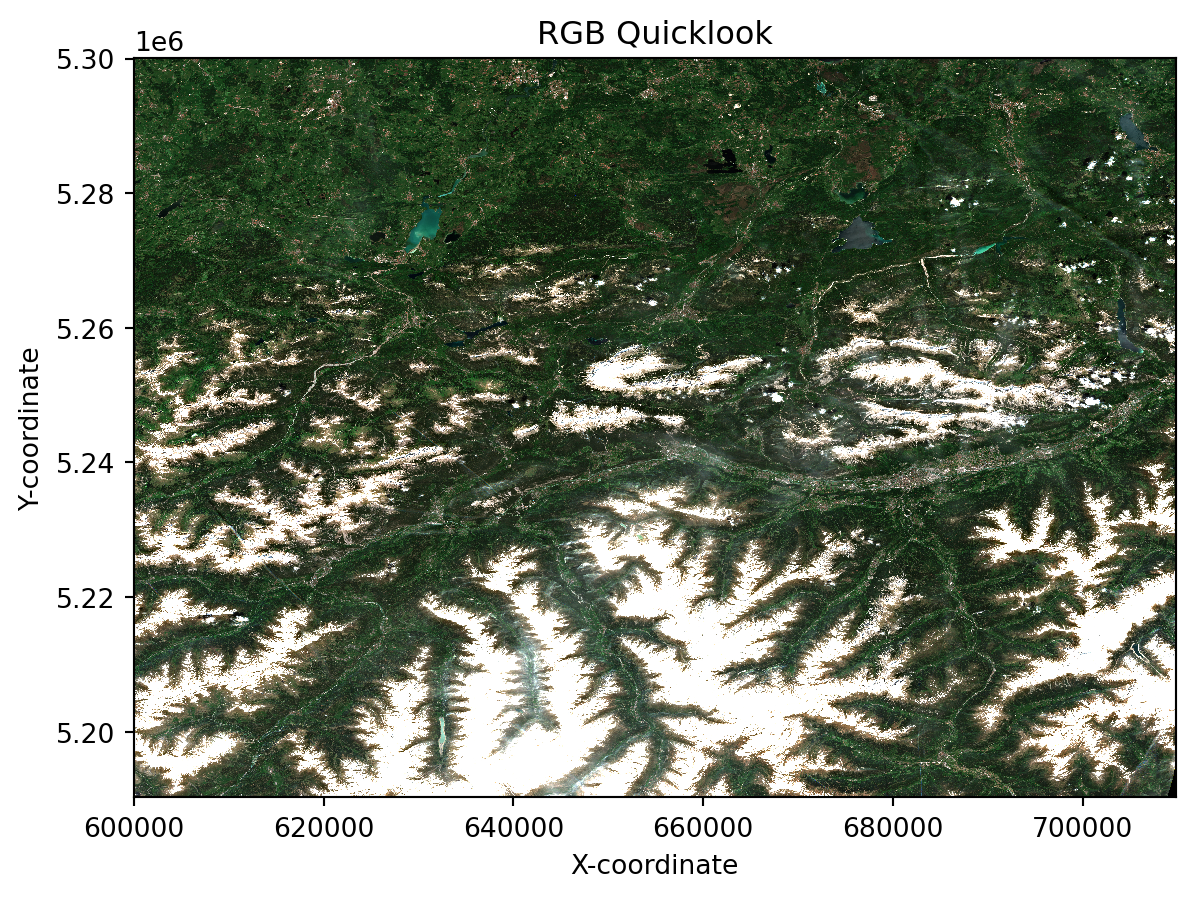
\includegraphics[keepaspectratio]{34_eopf_stac_xarray_tutorial_files/figure-pdf/cell-13-output-1.pdf}}

\section{Simple Data Analysis: Calculating
NDVI}\label{simple-data-analysis-calculating-ndvi}

Let us now do a simple analysis with the data from the EOPF Zarr STAC
Catalog. Let us calculate the Normalized Difference Vegetation Index
(NDVI).

First, we open the Zarr dataset specifically for the \textbf{red} (B04)
and \textbf{Near-Infrared} (B08) bands, which are crucial for the
calculation of the NDVI. We also specify \texttt{resolution=20} to
ensure we are working with the 20-meter resolution bands.

\begin{Shaded}
\begin{Highlighting}[]
\NormalTok{red\_nir }\OperatorTok{=}\NormalTok{ xr.open\_dataset(}
\NormalTok{    cloud\_storage,}
\NormalTok{    engine}\OperatorTok{=}\StringTok{"eopf{-}zarr"}\NormalTok{,}
\NormalTok{    chunks}\OperatorTok{=}\NormalTok{\{\},}
\NormalTok{    spline\_orders}\OperatorTok{=}\DecValTok{0}\NormalTok{,}
\NormalTok{    variables}\OperatorTok{=}\NormalTok{[}\StringTok{\textquotesingle{}b04\textquotesingle{}}\NormalTok{, }\StringTok{\textquotesingle{}b08\textquotesingle{}}\NormalTok{],}
\NormalTok{    resolution}\OperatorTok{=} \DecValTok{60}\NormalTok{,}
\NormalTok{)}
\end{Highlighting}
\end{Shaded}

In a next step, we cast the red (B04) and Near-Infrared (B08) bands to
floating-point numbers. This is important for accurate mathematical
operations, which we will conduct in the next cell.

\begin{Shaded}
\begin{Highlighting}[]
\NormalTok{red\_f }\OperatorTok{=}\NormalTok{ red\_nir.b04.astype(}\BuiltInTok{float}\NormalTok{)}
\NormalTok{nir\_f }\OperatorTok{=}\NormalTok{ red\_nir.b08.astype(}\BuiltInTok{float}\NormalTok{)}
\end{Highlighting}
\end{Shaded}

Now, we perform the initial steps for \textbf{NDVI} calculation: -
\texttt{sum\_bands}: Calculates the sum of the Near-Infrared and Red
bands. - \texttt{diff\_bands}: Calculates the difference between the
Near-Infrared and Red bands.

\begin{Shaded}
\begin{Highlighting}[]
\NormalTok{sum\_bands }\OperatorTok{=}\NormalTok{ nir\_f }\OperatorTok{+}\NormalTok{ red\_f}
\NormalTok{diff\_bands }\OperatorTok{=}\NormalTok{ nir\_f }\OperatorTok{{-}}\NormalTok{ red\_f}
\NormalTok{ndvi }\OperatorTok{=}\NormalTok{ diff\_bands }\OperatorTok{/}\NormalTok{ sum\_bands}
\end{Highlighting}
\end{Shaded}

To prevent division by zero errors in areas where both red and NIR bands
might be zero (e.g., water bodies or clouds), this line replaces any
\textbf{NaN} values resulting from division by zero with 0. This ensures
a clean and robust NDVI product.

\begin{Shaded}
\begin{Highlighting}[]
\NormalTok{ndvi }\OperatorTok{=}\NormalTok{ ndvi.where(sum\_bands }\OperatorTok{!=} \DecValTok{0}\NormalTok{, }\DecValTok{0}\NormalTok{)}
\end{Highlighting}
\end{Shaded}

In a final step, we can visualise the calculated NDVI.

\begin{Shaded}
\begin{Highlighting}[]
\NormalTok{ndvi.plot(cmap}\OperatorTok{=}\StringTok{\textquotesingle{}RdYlGn\textquotesingle{}}\NormalTok{, vmin}\OperatorTok{={-}}\DecValTok{1}\NormalTok{, vmax}\OperatorTok{=}\DecValTok{1}\NormalTok{)}
\NormalTok{plt.title(}\StringTok{\textquotesingle{}Normalized Difference Vegetation Index (NDVI)\textquotesingle{}}\NormalTok{)}
\NormalTok{plt.xlabel(}\StringTok{\textquotesingle{}X{-}coordinate\textquotesingle{}}\NormalTok{)}
\NormalTok{plt.ylabel(}\StringTok{\textquotesingle{}Y{-}coordinate\textquotesingle{}}\NormalTok{)}
\NormalTok{plt.grid(}\VariableTok{False}\NormalTok{) }\CommentTok{\# Turn off grid for image plots}
\NormalTok{plt.axis(}\StringTok{\textquotesingle{}tight\textquotesingle{}}\NormalTok{) }\CommentTok{\# Ensure axes fit the data tightly}

\CommentTok{\# Display the plot}
\NormalTok{plt.show()}
\end{Highlighting}
\end{Shaded}

\pandocbounded{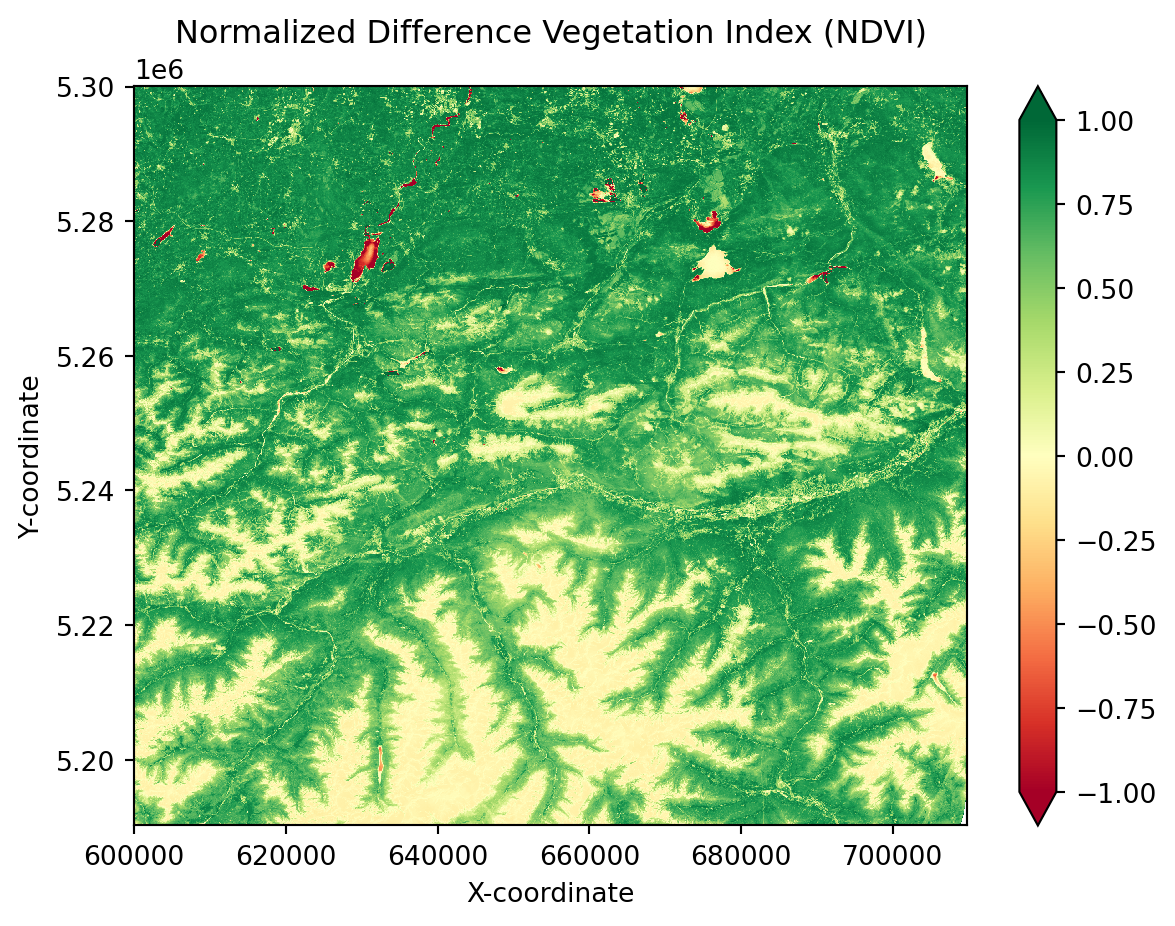
\includegraphics[keepaspectratio]{34_eopf_stac_xarray_tutorial_files/figure-pdf/cell-18-output-1.pdf}}

\section{💪 Now it is your turn}\label{now-it-is-your-turn-3}

With the foundations learned so far, you are now equipped to access
products from the EOPF Zarr STAC catalog. These are your tasks: \#\#\#
Task 1: Explore five additional Sentinel-2 Items for Innsbruck Replicate
the RGB quicklook and have an overview of the spatial changes.

\subsection{Task 2: Calculate NDVI}\label{task-2-calculate-ndvi}

Replicate the NDVI calculation for the additional Innsbruck items.

\subsection{Task 3: Applying more advanced analysis
techniques}\label{task-3-applying-more-advanced-analysis-techniques}

The EOPF STAC Catalog offers a wealth of data beyond Sentinel-2.
Replicate the search and data access for data from other collections.

\section{Conclusion}\label{conclusion-8}

In this section we established a connection to the
\href{https://stac.browser.user.eopf.eodc.eu/?.language=en}{EOPF
Sentinel Zarr Sample Service STAC Catalog} and directly accessed an EOPF
Zarr item with \texttt{xarray}. In the tutorial you are guided through
the process of opening hierarchical EOPF Zarr products using
\texttt{xarray}'s \texttt{DataTree}, a library designed for accessing
complex hierarchical data structures.

\section{What's next?}\label{whats-next-8}

This online resource is under active development. So stay tuned for
regular updates.

\part{{[}COMING SOON{]} Tools to work with EOPF Zarr}

\part{{[}COMING SOON{]} EOPF Zarr in Action}

\bookmarksetup{startatroot}

\chapter{\texorpdfstring{\textbf{Glossary}}{Glossary}}\label{glossary}

Here we introduce some helpful terms that are mentioned throughout the
EOPF 101.

\begin{longtable}[]{@{}
  >{\raggedright\arraybackslash}p{(\linewidth - 2\tabcolsep) * \real{0.5000}}
  >{\raggedright\arraybackslash}p{(\linewidth - 2\tabcolsep) * \real{0.5000}}@{}}
\toprule\noalign{}
\begin{minipage}[b]{\linewidth}\raggedright
Acronym
\end{minipage} & \begin{minipage}[b]{\linewidth}\raggedright
Definition
\end{minipage} \\
\midrule\noalign{}
\endhead
\bottomrule\noalign{}
\endlastfoot
\textbf{EOPF} & Earth Observation Processing Framework \\
\textbf{CDSE} & Copernicus Data Space Ecosystem \\
\textbf{CMP} & Core Python Modules \\
\textbf{HEALPix} & Hierarchical Equal Area isoLatitude Pixelation \\
\textbf{GDR} & Ground Range Detected \\
\textbf{SLC} & Single Look Complex \\
\textbf{NRB} & Normalized Radar Backscatter \\
\textbf{SAFE} & Standard Archive Format for Europe \\
\textbf{STAC} & Spatio Temporal Asset Catalog \\
\textbf{COG} & Cloud Optimised GeoTIFF \\
\textbf{Zarr} & Cloud-optimised version for \texttt{netCDF} and
\texttt{HDF5} formats, specifically designed for storing and accessing
large n-dimensional arrays \\
\end{longtable}

\bookmarksetup{startatroot}

\chapter{\texorpdfstring{\textbf{References}}{References}}\label{references}

The table below provides a categorized overview of key resources used
during the development of the EOPF 101 book.

\begin{longtable}[]{@{}
  >{\raggedright\arraybackslash}p{(\linewidth - 6\tabcolsep) * \real{0.0545}}
  >{\raggedright\arraybackslash}p{(\linewidth - 6\tabcolsep) * \real{0.1459}}
  >{\raggedright\arraybackslash}p{(\linewidth - 6\tabcolsep) * \real{0.2882}}
  >{\raggedright\arraybackslash}p{(\linewidth - 6\tabcolsep) * \real{0.5114}}@{}}
\toprule\noalign{}
\begin{minipage}[b]{\linewidth}\raggedright
Category
\end{minipage} & \begin{minipage}[b]{\linewidth}\raggedright
Resource Title
\end{minipage} & \begin{minipage}[b]{\linewidth}\raggedright
Description \& Context
\end{minipage} & \begin{minipage}[b]{\linewidth}\raggedright
Link
\end{minipage} \\
\midrule\noalign{}
\endhead
\bottomrule\noalign{}
\endlastfoot
\textbf{Sentinel Mission \& Product Specifications} & Sentinel-1 Level 1
Product Specification & Detailed specifications for Sentinel-1 Level 1
products. &
\href{https://s1.pages.eopf.copernicus.eu/s1-l12-rp/main/pfs/level_1_product_specification.html}{Available
here} \\
& Sentinel-2 - MSI - Level 2A Products & Auxiliary and data product
specifications for Sentinel-2 MSI Level 2A products. &
\href{https://s2.pages.eopf.copernicus.eu/pdfs-adfs/MSI/L2/PDFS_S2_MSI_L2.myst.html}{Available
here} \\
& Sentinel-3 -- Documentation (via CDSE) & Comprehensive documentation
for Sentinel-3 data products and mission. &
\href{https://documentation.dataspace.copernicus.eu/Data/SentinelMissions/Sentinel3.html}{Available
here} \\
\textbf{EOPF Platform \& Modules} & Supported Products Formats --- EOPF
- Core Python Modules & Guide to the product formats supported by the
Earth Observation Processing Framework's (EOPF) Core Python Modules. &
\href{https://cpm.pages.eopf.copernicus.eu/eopf-cpm/main/eoproduct-user-guide/supported_formats.html}{Available
here} \\
& EOPF Sentinel Zarr Samples Service STAC Catalog & A STAC (Spatio
Temporal Asset Catalog) for accessing Sentinel Zarr samples hosted by
EOPF. &
\href{https://stac.browser.user.eopf.eodc.eu/?.language=en}{Available
here} \\
& EOPF Sentinel Zarr Samples & Direct access to Sentinel data samples
stored in Zarr format within the EOPF ecosystem. &
\href{https://zarr.eopf.copernicus.eu/}{Available here} \\
\textbf{Data Formats \& Standards} & Zarr Documentation & Official
documentation for the Zarr format, a cloud-optimised standard for
n-dimensional arrays. & \href{https://zarr.dev/}{Available here} \\
& Introduction to the Zarr Format \textbar{} Copernicus Marine Help
Center & An introductory guide to the Zarr format, provided by the
Copernicus Marine Help Center. &
\href{https://help.marine.copernicus.eu/en/articles/10401542-introduction-to-the-zarr-format}{Available
here} \\
& Zarr + STAC & Article discussing the integration and benefits of
combining Zarr data with STAC catalogs. &
\href{https://element84.com/software-engineering/zarr-stac/}{Available
here} \\
& Is Zarr the new COG? & An insightful discussion comparing Zarr with
Cloud Optimised GeoTIFF (COG) for cloud-native geospatial data. &
\href{https://element84.com/software-engineering/is-zarr-the-new-cog/}{Available
here} \\
& About STAC & General information and principles behind the Spatio
Temporal Asset Catalog (STAC) specification. &
\href{https://stacspec.org/en/about/}{Available here} \\
\textbf{Cloud-Native Geospatial Initiatives} & Cloud-Native Geospatial
Forum (CNG) & The official website for the Cloud-Native Geospatial
Forum, promoting cloud-native approaches in geospatial. &
\href{https://cloudnativegeo.org/}{Available here} \\
\end{longtable}




\end{document}
